\documentclass[preprint,3p,10pt]{elsarticle}




%------------------------------------------------------------------------------
% FIGURES: CHOOSE ONE OPTION
%
% plots:       build standalone pdfs for figures, then use them
% plots-ext:   use existing pdfs for figures
% plots-none:  skip figures
%
%------------------------------------------------------------------------------
% hack for CVPR/ICCV style
\makeatletter
\@namedef{ver@everyshi.sty}{}
\makeatother

%------------------------------------------------------------------------------
% main packages
%\usepackage[dvipsnames,svgnames,x11names]{xcolor}
\usepackage{tikz}
\usetikzlibrary{arrows.meta,shapes,calc,matrix,fit,positioning,backgrounds,decorations.markings,fadings}
\usepackage{pgfplots}
\usepackage{pgfplotstable}
\usepgfplotslibrary{dateplot}
\pgfplotsset{compat=1.9}
\usepackage{xstring}

%------------------------------------------------------------------------------
% externalization: requires defining \finalcopy first

\usepgfplotslibrary{external}
% \tikzexternalize[prefix=fig/extern/]
\newcommand{\extfig}[2]{\tikzsetnextfilename{#1}{#2}}
\newcommand{\noextfig}[1]{\tikzset{external/export next={false}}{#1}}
\newcommand{\extdata}[1]{\input{#1}}
\IfBeginWith*{\jobname}{fig/extern/}{\finalcopy}{}

%-----------------------------------------------------------------------------
% tikz styles

\tikzstyle{every picture}+=[
	remember picture,
	every text node part/.style={align=center},
	every matrix/.append style={ampersand replacement=\&},
]
\tikzstyle{tight} = [inner sep=0pt,outer sep=0pt]
\tikzstyle{node}  = [draw,circle,tight,minimum size=12pt,anchor=center]
\tikzstyle{op}    = [draw,circle,tight]
\tikzstyle{dot}   = [fill,draw,circle,inner sep=1pt,outer sep=0]
\tikzstyle{pt}    = [fill,draw,circle,inner sep=1.5pt,outer sep=.2pt]
\tikzstyle{box}   = [draw,rectangle,inner sep=3pt]
\tikzstyle{high}  = [black!60]
\tikzstyle{group} = [high,box,opacity=.5]
\tikzstyle{dim1}  = [fill opacity=.3,text opacity=1]
\tikzstyle{dim2}  = [fill opacity=.5,text opacity=1]
\tikzstyle{dim3}  = [fill opacity=.7,text opacity=1]
\tikzstyle{rectc} = [tight,transform shape]
\tikzstyle{rect}  = [rectc,anchor=south west]

%-----------------------------------------------------------------------------
% framed figures

\newcommand{\framed}[3][1]{\extfig{#2}{\tikz{
	\node[tight](a){\fig[#1]{#3}};
	\node[tight,draw=gray,fit=(a)]{};
}}}

%-----------------------------------------------------------------------------
% pgfplots general options

\newcommand{\leg}[1]{\addlegendentry{#1}}

\tikzset{every mark/.append style={solid}}
\pgfplotsset{%smooth,
	grid=both, width=\columnwidth, try min ticks=5,
	every axis/.append style={font=\small},
	every axis plot/.append style={thick,mark=none,mark size=1.8,tension=0.18},
	legend cell align=left, legend style={fill opacity=0.8},
	xticklabel={\pgfmathprintnumber[assume math mode=true]{\tick}},
	yticklabel={\pgfmathprintnumber[assume math mode=true]{\tick}},
	nodes near coords math/.style={
	nodes near coords={\pgfmathprintnumber[assume math mode=true]{\pgfplotspointmeta}},
	},
}

\pgfplotsset{
	dash/.style={mark=o,dashed,opacity=0.6},
	dott/.style={mark=o,dotted,opacity=0.6},
	nolim/.style={enlargelimits=false},
	plain/.style={every axis plot/.append style={},nolim,grid=none},
}
%\pgfplotsset{scaled y ticks = false}
\newcommand{\kilo}[1]{\thisrow{#1}/1000}

%--------------------------------------------------------------------

% layers
\pgfdeclarelayer{bg4}
\pgfdeclarelayer{bg3}
\pgfdeclarelayer{bg2}
\pgfdeclarelayer{bg1}
\pgfdeclarelayer{fg1}
\pgfdeclarelayer{fg2}
\pgfdeclarelayer{fg3}
\pgfdeclarelayer{fg4}
\pgfsetlayers{bg4,bg3,bg2,bg1,main,fg1,fg2,fg3,fg4}

%------------------------------------------------------------------------------
% 3d drawing

\pgfkeys{/tikz/.cd, aspect/.store in=\aspect, aspect=1}
\pgfkeys{/tikz/.cd, depth/.store in=\depth, depth=.5}
\pgfkeys{/tikz/.cd, stepx/.store in=\step, stepx=1}

\tikzstyle{geom} = [line join=bevel,aspect=1,depth=.5,z={(\depth*\aspect,\depth)}]
\tikzstyle{wire} = [geom,draw,thick]

% 3d coordinates
\def\cx[#1,#2,#3]{#1}
\def\cy[#1,#2,#3]{#2}
\def\cz[#1,#2,#3]{#3}
\def\ex[#1,#2,#3]{#1,0,0}
\def\ey[#1,#2,#3]{0,#2,0}
\def\ez[#1,#2,#3]{0,0,#3}

% lines along x, y, or z
\newcommand{\zline}[3][]{%
\path[geom,#1] #2 -- +(\cx[#3],\cy[#3]);
}
\newcommand{\yline}[3][]{%
\path[geom,#1,shift={#2},xslant=\aspect]
	(0,0) -- +(\cx[#3],\depth*\cz[#3]);
}
\newcommand{\xline}[3][]{%
\path[geom,#1,shift={#2},yslant=1/\aspect]
	(0,0) -- +(\aspect*\depth*\cz[#3],\cy[#3]);
}

% rectangles / grids along x, y, or z
\newcommand{\zrect}[3][]{%
\path[geom,#1] #2 rectangle +(\cx[#3],\cy[#3]);
}
\newcommand{\yrect}[3][]{%
\path[geom,#1,shift={#2},xslant=\aspect]
	(0,0) rectangle +(\cx[#3],\depth*\cz[#3]);
}
\newcommand{\xrect}[3][]{%
\path[geom,#1,shift={#2},yslant=1/\aspect]
	(0,0) rectangle +(\aspect*\depth*\cz[#3],\cy[#3]);
}
\newcommand{\xgrid}[3][]{%
\path[geom,#1,shift={#2},yslant=1/\aspect,xstep=\aspect*\depth*\step]
	(0,0) grid +(\aspect*\depth*\cz[#3],\cy[#3]);
}

% parallepiped
\newcommand{\para}[4][]{%
\zrect[#1]{(#3)}{#4}                 % front
\yrect[#1]{($(#3)+(\ey[#4])$)}{#4}   % top
\xrect[#1]{($(#3)+(\ex[#4])$)}{#4}   % right
\path[geom]
	(#3) coordinate(#2-southwest)
	($(#3)+(#4)$) coordinate(#2-northeast)
	($(#3)+(\ey[#4])$) coordinate(#2-northwest)
	($(#3)+(#4)-(\ey[#4])$) coordinate(#2-southeast)
	($(#3)+.5*(\ex[#4])$) coordinate(#2-south)
	($(#3)+(#4)-.5*(\ex[#4])$) coordinate(#2-north)
	($(#3)+.5*(\ex[#4])+.5*(#4)$) coordinate(#2-center)
	(#2-southwest |- #2-center) coordinate(#2-west)
	(#2-center -| #2-northeast) coordinate(#2-east)
	;
}

%------------------------------------------------------------------------------
% space before \paragraph (default 4.05ex)
% \makeatletter
% \renewcommand\paragraph{\@startsection{paragraph}{4}{\z@}{1ex}{-1em}{\normalfont\normalsize\bfseries}}
% \makeatother
%------------------------------------------------------------------------------
% \usepackage[numbers,sort&compress]{natbib}
\usepackage{natbib}
\usepackage{times}
\usepackage{epsfig}
\usepackage{graphicx}
\usepackage{amsmath}
\usepackage{amssymb}
\usepackage{xspace}
\usepackage{color}
% \usepackage{setspace} 

\usepackage{enumitem}
\usepackage{multirow}
\usepackage{array,booktabs}
\usepackage{bbm}
\usepackage{colortbl}

\usepackage[pagebackref=true,breaklinks=true,colorlinks,bookmarks=false]{hyperref}

% Support for easy cross-referencing
\usepackage[capitalize]{cleveref}
\crefname{section}{Sec.}{Secs.}
\Crefname{section}{Section}{Sections}
\Crefname{table}{Table}{Tables}
\crefname{table}{Tab.}{Tabs.}

\journal{Pattern Recognition}
% \doublespacing
\linespread{2}
\begin{document}



\newcommand{\head}[1]{{\smallskip\noindent\textbf{#1}}}
\newcommand{\alert}[1]{{\color{red}{#1}}}
\newcommand{\sm}{\scriptsize}
\newcommand{\eq}[1]{(\ref{eq:#1})}

\newcommand{\Th}[1]{\textsc{#1}}
\newcommand{\mr}[2]{\multirow{#1}{*}{#2}}
\newcommand{\mc}[2]{\multicolumn{#1}{c}{#2}}
\newcommand{\tb}[1]{\textbf{#1}}
\newcommand{\ch}{\checkmark}

\newcommand{\red}[1]{{\color{red}{#1}}}
\newcommand{\blue}[1]{{\color{blue}{#1}}}
\newcommand{\green}[1]{{\color{green}{#1}}}
\newcommand{\gray}[1]{{\color{gray}{#1}}}

\newcommand{\citeme}[1]{\red{[XX]}}
\newcommand{\refme}[1]{\red{(XX)}}

\newcommand{\fig}[2][1]{\includegraphics[width=#1\linewidth]{fig/#2}}
\newcommand{\figh}[2][1]{\includegraphics[height=#1\linewidth]{fig/#2}}


\newcommand{\tran}{^\top}
\newcommand{\mtran}{^{-\top}}
\newcommand{\zcol}{\mathbf{0}}
\newcommand{\zrow}{\zcol\tran}

\newcommand{\ind}{\mathbbm{1}}
\newcommand{\expect}{\mathbb{E}}
\newcommand{\nat}{\mathbb{N}}
\newcommand{\zahl}{\mathbb{Z}}
\newcommand{\real}{\mathbb{R}}
\newcommand{\proj}{\mathbb{P}}
\newcommand{\prob}{\operatorname{P}}
\newcommand{\normal}{\mathcal{N}}

\newcommand{\mif}{\textrm{if}\ }
\newcommand{\other}{\textrm{otherwise}}
\newcommand{\minimize}{\textrm{minimize}\ }
\newcommand{\maximize}{\textrm{maximize}\ }
\newcommand{\st}{\textrm{subject\ to}\ }

\newcommand{\id}{\operatorname{id}}
\newcommand{\const}{\operatorname{const}}
\newcommand{\sgn}{\operatorname{sgn}}
\newcommand{\var}{\operatorname{Var}}
\newcommand{\mean}{\operatorname{mean}}
\newcommand{\trace}{\operatorname{tr}}
\newcommand{\diag}{\operatorname{diag}}
\newcommand{\vect}{\operatorname{vec}}
\newcommand{\cov}{\operatorname{cov}}
\newcommand{\sign}{\operatorname{sign}}
\newcommand{\prj}{\operatorname{proj}}

\newcommand{\softmax}{\operatorname{softmax}}
\newcommand{\clip}{\operatorname{clip}}

\newcommand{\defn}{\mathrel{:=}}
\newcommand{\peq}{\mathrel{+\!=}}
\newcommand{\meq}{\mathrel{-\!=}}

\newcommand{\floor}[1]{\left\lfloor{#1}\right\rfloor}
\newcommand{\ceil}[1]{\left\lceil{#1}\right\rceil}
\newcommand{\inner}[1]{\left\langle{#1}\right\rangle}
\newcommand{\norm}[1]{\left\|{#1}\right\|}
\newcommand{\abs}[1]{\left|{#1}\right|}
\newcommand{\frob}[1]{\norm{#1}_F}
\newcommand{\card}[1]{\left|{#1}\right|\xspace}

\newcommand{\diff}{\mathrm{d}}
\newcommand{\der}[3][]{\frac{\diff^{#1}#2}{\diff#3^{#1}}}
\newcommand{\ider}[3][]{\diff^{#1}#2/\diff#3^{#1}}
\newcommand{\pder}[3][]{\frac{\partial^{#1}{#2}}{\partial{{#3}^{#1}}}}
\newcommand{\ipder}[3][]{\partial^{#1}{#2}/\partial{#3^{#1}}}
\newcommand{\dder}[3]{\frac{\partial^2{#1}}{\partial{#2}\partial{#3}}}

\newcommand{\wb}[1]{\overline{#1}}
\newcommand{\wt}[1]{\widetilde{#1}}

\def\xssp{\hspace{1pt}}
\def\ssp{\hspace{3pt}}
\def\msp{\hspace{5pt}}
\def\lsp{\hspace{12pt}}

\newcommand{\cA}{\mathcal{A}}
\newcommand{\cB}{\mathcal{B}}
\newcommand{\cC}{\mathcal{C}}
\newcommand{\cD}{\mathcal{D}}
\newcommand{\cE}{\mathcal{E}}
\newcommand{\cF}{\mathcal{F}}
\newcommand{\cG}{\mathcal{G}}
\newcommand{\cH}{\mathcal{H}}
\newcommand{\cI}{\mathcal{I}}
\newcommand{\cJ}{\mathcal{J}}
\newcommand{\cK}{\mathcal{K}}
\newcommand{\cL}{\mathcal{L}}
\newcommand{\cM}{\mathcal{M}}
\newcommand{\cN}{\mathcal{N}}
\newcommand{\cO}{\mathcal{O}}
\newcommand{\cP}{\mathcal{P}}
\newcommand{\cQ}{\mathcal{Q}}
\newcommand{\cR}{\mathcal{R}}
\newcommand{\cS}{\mathcal{S}}
\newcommand{\cT}{\mathcal{T}}
\newcommand{\cU}{\mathcal{U}}
\newcommand{\cV}{\mathcal{V}}
\newcommand{\cW}{\mathcal{W}}
\newcommand{\cX}{\mathcal{X}}
\newcommand{\cY}{\mathcal{Y}}
\newcommand{\cZ}{\mathcal{Z}}

\newcommand{\vA}{\mathbf{A}}
\newcommand{\vB}{\mathbf{B}}
\newcommand{\vC}{\mathbf{C}}
\newcommand{\vD}{\mathbf{D}}
\newcommand{\vE}{\mathbf{E}}
\newcommand{\vF}{\mathbf{F}}
\newcommand{\vG}{\mathbf{G}}
\newcommand{\vH}{\mathbf{H}}
\newcommand{\vI}{\mathbf{I}}
\newcommand{\vJ}{\mathbf{J}}
\newcommand{\vK}{\mathbf{K}}
\newcommand{\vL}{\mathbf{L}}
\newcommand{\vM}{\mathbf{M}}
\newcommand{\vN}{\mathbf{N}}
\newcommand{\vO}{\mathbf{O}}
\newcommand{\vP}{\mathbf{P}}
\newcommand{\vQ}{\mathbf{Q}}
\newcommand{\vR}{\mathbf{R}}
\newcommand{\vS}{\mathbf{S}}
\newcommand{\vT}{\mathbf{T}}
\newcommand{\vU}{\mathbf{U}}
\newcommand{\vV}{\mathbf{V}}
\newcommand{\vW}{\mathbf{W}}
\newcommand{\vX}{\mathbf{X}}
\newcommand{\vY}{\mathbf{Y}}
\newcommand{\vZ}{\mathbf{Z}}

\newcommand{\va}{\mathbf{a}}
\newcommand{\vb}{\mathbf{b}}
\newcommand{\vc}{\mathbf{c}}
\newcommand{\vd}{\mathbf{d}}
\newcommand{\ve}{\mathbf{e}}
\newcommand{\vf}{\mathbf{f}}
\newcommand{\vg}{\mathbf{g}}
\newcommand{\vh}{\mathbf{h}}
\newcommand{\vi}{\mathbf{i}}
\newcommand{\vj}{\mathbf{j}}
\newcommand{\vk}{\mathbf{k}}
\newcommand{\vl}{\mathbf{l}}
\newcommand{\vm}{\mathbf{m}}
\newcommand{\vn}{\mathbf{n}}
\newcommand{\vo}{\mathbf{o}}
\newcommand{\vp}{\mathbf{p}}
\newcommand{\vq}{\mathbf{q}}
\newcommand{\vr}{\mathbf{r}}
\newcommand{\Vs}{\mathbf{s}}
\newcommand{\vt}{\mathbf{t}}
\newcommand{\vu}{\mathbf{u}}
\newcommand{\vv}{\mathbf{v}}
\newcommand{\vw}{\mathbf{w}}
\newcommand{\vx}{\mathbf{x}}
\newcommand{\vy}{\mathbf{y}}
\newcommand{\vz}{\mathbf{z}}

\newcommand{\vone}{\mathbf{1}}
\newcommand{\vzero}{\mathbf{0}}

\newcommand{\valpha}{{\boldsymbol{\alpha}}}
\newcommand{\vbeta}{{\boldsymbol{\beta}}}
\newcommand{\vgamma}{{\boldsymbol{\gamma}}}
\newcommand{\vdelta}{{\boldsymbol{\delta}}}
\newcommand{\vepsilon}{{\boldsymbol{\epsilon}}}
\newcommand{\vzeta}{{\boldsymbol{\zeta}}}
\newcommand{\veta}{{\boldsymbol{\eta}}}
\newcommand{\vtheta}{{\boldsymbol{\theta}}}
\newcommand{\viota}{{\boldsymbol{\iota}}}
\newcommand{\vkappa}{{\boldsymbol{\kappa}}}
\newcommand{\vlambda}{{\boldsymbol{\lambda}}}
\newcommand{\vmu}{{\boldsymbol{\mu}}}
\newcommand{\vnu}{{\boldsymbol{\nu}}}
\newcommand{\vxi}{{\boldsymbol{\xi}}}
\newcommand{\vomikron}{{\boldsymbol{\omikron}}}
\newcommand{\vpi}{{\boldsymbol{\pi}}}
\newcommand{\vrho}{{\boldsymbol{\rho}}}
\newcommand{\vsigma}{{\boldsymbol{\sigma}}}
\newcommand{\vtau}{{\boldsymbol{\tau}}}
\newcommand{\vupsilon}{{\boldsymbol{\upsilon}}}
\newcommand{\vphi}{{\boldsymbol{\phi}}}
\newcommand{\vchi}{{\boldsymbol{\chi}}}
\newcommand{\vpsi}{{\boldsymbol{\psi}}}
\newcommand{\vomega}{{\boldsymbol{\omega}}}

\newcommand{\rLambda}{\mathrm{\Lambda}}
\newcommand{\rSigma}{\mathrm{\Sigma}}

\newcommand{\vLambda}{\bm{\rLambda}}
\newcommand{\vSigma}{\bm{\rSigma}}

\makeatletter
\newcommand*\bdot{\mathpalette\bdot@{.7}}
\newcommand*\bdot@[2]{\mathbin{\vcenter{\hbox{\scalebox{#2}{$\m@th#1\bullet$}}}}}
\makeatother

\makeatletter
\DeclareRobustCommand\onedot{\futurelet\@let@token\@onedot}
\def\@onedot{\ifx\@let@token.\else.\null\fi\xspace}

\def\eg{\emph{e.g}\onedot} \def\Eg{\emph{E.g}\onedot}
\def\ie{\emph{i.e}\onedot} \def\Ie{\emph{I.e}\onedot}
\def\cf{\emph{cf}\onedot} \def\Cf{\emph{Cf}\onedot}
\def\etc{\emph{etc}\onedot} \def\vs{\emph{vs}\onedot}
\def\wrt{w.r.t\onedot} \def\dof{d.o.f\onedot} \def\aka{a.k.a\onedot}
\def\etal{\emph{et al}\onedot}
\makeatother

\newcommand{\relu}{\operatorname{ReLU}}
\newcommand{\gap}{\operatorname{GAP}}
\newcommand{\up}{\operatorname{Up}}
\newcommand{\ce}{\operatorname{CE}}

\newcommand{\cam}{\textrm{CAM}}
\newcommand{\gcam}{\textrm{Grad-CAM}}
\newcommand{\scam}{\textrm{Score-CAM}}

\newcommand{\mae}{\textrm{MAE}}
\newcommand{\mse}{\textrm{MSE}}
\newcommand{\hi}{\textrm{HI}}



\newcommand{\ronan}[1]{#1}
\newcommand{\iavr}[1]{#1}
\newcommand{\stephane}[1]{#1}
\newcommand{\redred}[1]{#1}
\newcommand{\hw}[1]{{\color{olive}{#1}}}
% \newcommand{\modify}[1]{{\color{blue}{#1}}}
\newcommand{\modify}[1]{{{#1}}}


\begin{frontmatter}
\title{Opti-CAM: Optimizing saliency maps for interpretability}


\author[1]{Hanwei Zhang}
\ead{hanwei.zhang@lis-lab.fr}
% \cormark[1]
\author[1]{Felipe Torres}
\ead{felipe.torres@lis-lab.fr}
\author[1]{Ronan Sicre}
\ead{ronan.sicre@lis-lab.fr}
\author[2]{Yannis Avrithis}
\ead{yannis@avrithis.net}
\author[1]{Stephane Ayache}
\ead{stephane.ayache@univ-amu.fr}


% Address/affiliation
\affiliation[1]{organization={Centrale Marseille, Aix Marseille Univ, CNRS, LIS},
            % addressline={52 Av. Escadrille Normandie Niemen}, 
            city={Marseille},
%          citysep={}, % Uncomment if no comma needed between city and postcode
            postcode={13397}, 
            % state={},
            country={France}}

\affiliation[2]{organization={Institute of Advanced Research on Artificial Intelligence (IARAI)},
            % addressline={Landstraßer Hauptstraße 5 Eingang, u. Viaduktgasse 16, 2. Stock}, 
            city={Vienna},
%          citysep={}, % Uncomment if no comma needed between city and postcode
            postcode={1030}, 
            % state={},
            country={Austria}}



\begin{abstract}
Methods based on \emph{class activation maps} (CAM) provide a simple mechanism to interpret predictions of convolutional neural networks by using linear combinations of feature maps as saliency maps. By contrast, masking-based methods optimize a saliency map directly in the image space or learn it by training another network on additional data.

In this work we introduce Opti-CAM, combining ideas from CAM-based and masking-based approaches. Our saliency map is a linear combination of feature maps, where weights are optimized per image such that the logit of the masked image for a given class is maximized. We also fix a fundamental flaw in two of the most common evaluation metrics of attribution methods. On several datasets, Opti-CAM largely outperforms other CAM-based approaches according to the most relevant classification metrics. We provide empirical evidence supporting that localization and classifier interpretability are not necessarily aligned.
\end{abstract}

% \begin{graphicalabstract}
% \end{graphicalabstract}

\begin{highlights}
\item We introduce Opti-CAM, a simple model for saliency map generation that combines ideas from CAM-based and masking-based approaches. Opti-CAM does not need any extra data, network or training.

\item Compared with gradient-free methods, it finds the optimal feature map weights and is on par or faster, assuming that the number of iterations is less than the number of channels.
\item We introduce a new evaluation metric, \emph{\agf} ($\AG$), to be paired with \emph{average drop} ($\AD$) as a replacement of \emph{average increase} ($\AI$).
\item On several datasets,	we improve the state of the art by a large margin, \redred{reaching near-perfect performance} according to the most relevant classification metrics.
\item We shed more light into how a classifier may exploit background context.
\end{highlights}

\begin{keyword}
Interpretability; Explainable AI; Saliency map; Class activation maps; Computer vision; 
\end{keyword}
\end{frontmatter}


%--------------------------------------------------------------------------------------------------
\addchap{Introduction}
%\addcontentsline{toc}{chapter}{Introduction}
\noindent Amongst the sensory information that the brain processes, visual stimuli accounts 
for 90\% of data analyzed \autocite{potter2014detecting}, while consuming a great amount of energy 
in human metabolism (\cite{phelps1981metabolic}). It is argued that a big influence on the 
brain evolution was as a result of improving the capacity to process this kind of data and the 
ensuing  pattern recognition (\cite{mattson2014superior}). 
Currently, these shapes and forms have evolved too: it is no longer common for a human in most 
metropolitan areas, the need to scan the environment for faces that could reveal a potential 
predator; for a change, the patterns that we now seek to unravel also contain products of our own 
imagination: digits and characters, geometrical shapes.\\

\paragraph{Visual Recognition} Understanding the processes behind visual recognition has been a 
prominent research question throughout human history. From the preliminary questionings by greek  
philosphers (\cite{finger2001origins}) to physics based studies like those by Newton and Locke 
(\cite{swenson2010optics}), and more recently with theories like \textit{Unconscious Inference} 
(\cite{gullstrand1909hemholtz}) and \textit{Gestalt} (\cite{wagemans2012century}), many proposals 
to understand and describe this process have been brought forth. Moreover, vision recogniton is not 
only studied in fields like physics, medicine and psychology; 
with the advent of computer science, computational approaches and theories started emerging 
regarding this domain. One such study that proved seminal in this domain is that carried out by 
David Marr (\cite{poggio1981marr}, \cite{marr2010vision}). Most notably, Marr addressed vision on 
three levels: comptational, algorithmic and implementation. In particular, upon the computational 
level, Marr pondered around issues that the visual system answers and their explanation; this 
ultimately led to the formulation of fundamental tasks within computer vision such as object 
recognition and reconstruction. Over the past decade great advancements were made on computer 
vision. In particular with the optimization and popularization of \gls{gpu}, models requiring 
a strong computational power became accesible for researchers. To be specific, the framework 
developed by Yann LeCun (\cite{lecun1998gradient}) got revitalized in 2012 with the introduction of 
AlexNet (\cite{krizhevsky2012imagenet}) where proper leverage of these machines outclassed that of 
more traditional machine learning models, Chapter \ref{ch:rel} discusses this in more depth. 
In this short span of time, several groundbreaking architectures have been proposed, in 
particular the ResNet family (\cite{he2016deep}) has remained relevant given its properties
(\cite{wightman2021resnet}); furthermore, with the introduction of the transformer architecture 
(\cite{vaswani2017attention}) this field of research recieved a new impulse and more powerful 
models based upon its functional unit are being brought forth.\\

\noindent It is not only with the increase of computational power that computer vision has improved over time. 
With the developement, popularization and spread of the internet; large collections of data have been 
formed. These aggregations can be extremely specific for a given end, or 
quite general representing the common interests of its users. Over time, these compilations have 
continued to grow both in volume and variety; still, several curated collections are introduced by 
researchers to experiment and control the development of models such as MNIST (\cite{lecun1998gradient}),
BSDS (\cite{MartinFTM01}), Pascal VOC (\cite{pascal-voc-2012}) and most notably, 
ImageNet (\cite{ILSVRC15}) and MS-COCO (\cite{lin2014microsoft}). Additionally, data collection is
an ongoing and a never ending process; as such, the idea of a dataset containing all types of 
information is no longer deemded a dream but a reality that might come true aided by Big Data in 
the foreseeable future \autocite{chen2014big}.\\

\noindent Taking into consideration the aforementioned  increase on  both compute power and data 
availability, deep learning based models have been steadily adopted and assimiliated within society; 
nowadays its no longer so much a question \textit{whether can a model achieve a given task}, but 
rather a question on \textit{how can this given model perform this task}. Providing an answer to 
this question is paramount as human lives are now being directly affected by such kind of models. 
The main issue behind understanding deep models, lies within the size and complexity of deep 
architecttures, where providing interpretable explanations has lead to the surge of a novel field 
of research (\cite{guidotti2018survey}, \cite{bodria2021benchmarking}).

\paragraph{Interpretability}
To begin discussing about interpretability, one must ponder around its definition. 
Over the last decade, many authors have attempted to address to this question. One 
of the most notable discussions can be found within \emph{The Mythos of Model Interpretability} 
(\cite{mythos_interp}). In this work, Lipton argues that for a model to be interpretable it must 
display two properties, \emph{Transparency} and \emph{Post-Hoc Interpretability}. In one hand, 
\textit{Transparency} answers questions regarding the model structure, training and inference 
processes; while on another hand, \textit{Post-Hoc Interpretability} relates to the explanations 
and information that can be drawn of the model itself.

\noindent Considering these properties, we observe that as machine learning models grew in 
complexity; their transparent properties vanished proportionaly to their size. It can be argued 
that traditional models offer themselves to  transparency due to their straightforward formulation 
and inherent properties. Conversely, in terms of post-hoc interpretations, methods like decision 
trees \cite{breiman2017classification} can be pruned to study their performance by removing 
branches (\cite{lakkaraju2016interpretable},\cite{mothilal2020explaining}). 
On another hand, established techniques such as Principal Component Analysis \gls{pca} 
(\cite{wold1987principal}), can be used to gain insight within data leading to a prediction.\\

\noindent When studying deep models, we find that it is after their size and complexity that their 
interpretable propierties get hindered. Common Convolutional Neural Networks \glspl{cnn} 
rely convolution as their corner stone, coupled with non-linear operations such as 
ReLU (\cite{fukushima1975cognitron}), Sigmoid, and Softmax (\cite{hopfield1985neural}) among others.
This aggregation of convolutions on one hand enables these models to process large quantities of 
data, and to a certain extent generalize; however, it also results in an extensive parameter count,
often reaching of millions, and most recently, even billions (\cite{openai_compute}). The 
computational load required for inference, typically measured in \gls{gflops} further compounds 
complexity.\\

\noindent Among the properties proposed by Lipton, we observe that offering model transparency is a 
rather challenging task. While understanding the behaviour of convolutions and 
self-attention might seem straightforward, it is their aggregation and subsequent flow of information what 
makes this process intricate. Moreover, transparency encompases aspects related to both
inference and training. In this regard, while deep learning research is often seen as an open field;
complete transparency is often disregarded as some authors frequently omit key details in their 
descriptions and methodologies. 

In contrast to transparency, providing post-hoc interpretations from deep models is a 
thriving field, where many of the challenges found within transparency are no longer found.
Within this field, various approaches have been proposed to achieve post-hoc interpretability,
including input masking (\cite{petsiuk2018rise}), attribution generation (\cite{NIPS2017_7062}, 
\cite{zhou2016learning}) and model perturbations 
(\cite{fong2017interpretable}, \cite{fong2019understanding}). Furthermore, the development of 
evaluation methodologies for these approaches has continued in tandem with them 
(\cite{choe2020evaluating}, \cite{chattopadhay2018grad}). Chapter \ref{ch:rel} delves deeper into 
these works. 

\paragraph{Dissertation Outline}
%\addcontentsline{toc}{section}{Dissertation Outline}
\noindent This dissertation is organized in the following manner: In Chapter \ref{ch:rel} we 
introduce a background for image recognition models (Section \ref{rel:sec_imrecon}) and the ensuing 
approaches developed to study the interpretability on them (Section \ref{rel:sec_int}). 
Additionally, we introduce evaluation procedures for these approaches which will be further used to 
evaluate ourproposals.\\

\noindent In Chapter \ref{ch:opticam}, we propose Opti-CAM as a methodology that generates 
optimized saliency maps highlighting the relevant regions on an image towards image classification. 
In Section \ref{sec:av_gain} we extend existing evaluation metrics with a novel measurement for 
model coinfidence. 
In Sections \ref{sec:oc_qual} and \ref{sec:oc_quant} we evaluate the effect of these contributions 
towards interpretability assessment.\\

\noindent Chapter \ref{ch:castream} introduces the Cross Attention Stream, an approach that boosts existing 
architectures interpretable properties. We ste up the modulus of this approach in 
Section \ref{sec:ca_defn} alongside its deployment on Section \ref{sec:ca_design}. 
In Sections \ref{sec:ca_qual} and \ref{sec:ca_quant} we demonstrate the benefits of using this
proposal.\\

\noindent Chapter \ref{ch:grad} characterizes a gradient denoising approach with a gradient denoising 
methodology as an approach to enhance the trainining procedure of current models while improving 
interpretability properties. In Section \ref{sec:grad_defn}, we define the gradient denoising 
protocol alongside the regularization proposals to do so.
Sections \ref{sec:grad_qual} and \ref{sec:grad_quant} illustrate the effects of this paradigmn
in the trained models and its effects on interpretability.\\

\noindent Chapter \ref{ch:zip} raises the Zero-Information algorithm and its usage as a substitute
for mask-dependent evaluation proposals. Section \ref{sec:zip_algo} develops this 
method. Section \ref{sec:zip_insdel} demonstrates its incorporation of this 
algorithm onto evaluation protocols. Section \ref{sec:zip_qual} displays
the effect of this approach when applied to mask patches on images. Section 
\ref{sec:zip_benchmark} displays the results of benchmarking these protocols 
with this approach. \\
    
\noindent Finally, we draw conclusions on our work and detail future research perspectives.
\section{Related Work}

\subsection{Interpretability}

To open up the black-box behavior of deep neural networks, model interpretability is mainly investigated along two directions~\citep{lipton18, guidotti2018survey, zhang2021survey}:
\begin{enumerate}[itemsep=2pt, parsep=0pt, topsep=3pt]
	\item \emph{Post-hoc interpretability} considers the model as a black-box and provides explanations based on inputs and outputs, without modifying the model or its training process.
	\item \emph{Transparency} modifies the model or the training process to better explain the behavior of the inner parts of the model.
\end{enumerate}

\paragraph{Post-hoc interpretability}

Approaches can be grouped into a number of possibly overlapping categories. \emph{Gradient-based methods}~\citep{adebayo2018local, springenberg2014striving, baehrens2010explain, simonyan2013deep, smilkov2017smoothgrad, bach2015pixel, sundararajan2017axiomatic} use the gradient of a target class score with respect to the input to compute the contribution of different input regions to the prediction. \emph{CAM-based methods}~\citep{DBLP:journals/corr/abs-1910-01279, DBLP:journals/corr/abs-1710-11063, DBLP:journals/corr/SelvarajuDVCPB16, fu2020axiom, jiang2021layercam, ramaswamy2020ablation} compute saliency maps as a linear combination of feature maps, with different definitions for the weights. \emph{Occlusion or masking-based methods}~\citep{petsiuk2018rise, fong2017interpretable, fong2019understanding, schulz2020restricting, ribeiro2016should} apply a number of candidate masks in the input space, measure their effect on the prediction and then combine them into a saliency map. Masking in feature space has been explored too~\cite{schulz2020restricting}. Finally, \emph{learning-based methods}~\citep{chang2018explaining, dabkowski2017real, phang2020investigating, zolna2020classifier, schulz2020restricting} learn an additional network or branch on extra data to produce an explanation map for a given input. 

Our method shares similarities with learning-based methods. In particular, we train an additional branch on the same training data as the network we aim to explain, but we only use the standard classification loss and we do not provide any explanation as output. Our method is also similar to CAM-based and masking-based methods exactly because we show that attention-based pooling is the same as masking in the feature space with weights obtained by a CAM-based saliency map.

\paragraph{Transparency}

Approaches are grouped in a number of categories according to the type of the given explanation. \emph{Rule-based methods}~\citep{wu2018beyond, wu2020regional} train a decision tree as a surrogate regularization term to force a network to be easily approximated by a decision tree.
% or learn a set of logit rules as an explanation~\citep{azzolin2022global}.
\emph{Hidden semantics-based methods}~\citep{bau2017network, zhou2018interpreting, zhang2018interpretable, zhou2014object} aim to make a convolutional network learn disentangled hidden semantics with hierarchical structure or object-level concepts.
\emph{Prototype-based methods}~\citep{li2018deep, chen2019looks} learn a set of prototypes or parts as an intermediate representation in the network, which can be aligned with categories. \emph{Attribution-based methods}~\citep{ismail2021improving, Zhou_2022_BMVC, ross2017right, ghaeini2019saliency} usually modify the architecture of a network or the training process to help post-hoc methods produce better saliency maps. Unlike~\citep{ross2017right, ghaeini2019saliency}, saliency guided localization~\citep{Zhou_2022_BMVC} does not need ground truth explanations but replaces them with information bottleneck attribution~\citep{schulz2020restricting}. Finally, saliency-guided training~\citep{ismail2021improving} minimizes the KL divergence between the output of original and masked images.

Our method belongs to attribution-based methods. We introduce a learnable cross-attention stream into the network as a pooling mechanism to replace \gap. As a result, post-hoc attribution-based methods can provide a better explanation. Although the network is modified, the training process is not: the network and classifier are pretrained and kept frozen while we learn the paramaters of our stream.

%------------------------------------------------------------------------------

\subsection{Attention-based architectures}

Attention is a powerful mechanism that has been introduced into convolutional networks in several ocaasions~\citep{bello2019attention, ramachandran2019stand, shen2020global}. With the success of vision transformers (ViT)~\citep{dosovitskiy2020image}, fully attention-based architectures are now competitive with convolutional networks. To benefit from both self-attention and convolutional layers, some hybrid architectures employ convolutional layers before the vision transformer~\citep{graham2021levit,xiao2021early}. Others, such as Swin~\citep{liu2021swin} and PiT~\citep{heo2021rethinking}, introduce a pyramid structure to share local spatial information while reducing the spatial resolution, as in convolutional networks. 

Conformer~\citep{peng2021conformer} proposes a dual network structure to retrain and fuse local convolutional features with global representations. Our method merely provides a simple attention-based pooling mechanism inspired by transformers that can work with any architecture, even pretrained and frozen. SCOUTER~\citep{li2021scouter} uses slot attention~\cite{locatello2020object} to build a class specific pooling mechanism, which does not scale well to more than 20 classes. Our mechanism is based standard cross attention, it is class agnostic and scales up to 1000 classes, improving post-hoc interpretability without degrading classification accuracy. PatchConvNet~\citep{touvron2021augmenting} replaces global average pooling by an attention-based pooling layer. Our method is similar in this respect, but uses information collected from the entire network by a parallel processing stream. We introduce our mechanism into any convolutional network and study its effect on post-hoc interpretability.








\section{Opti-CAM}
\label{sec:opticam}

\subsection{Preliminaries}
\label{sec:prelim}

\paragraph{Notation}
\label{sec:notation}

Consider a classifier network $f: \cX \to \real^C$ that maps an input image $\vx \in \cX$ to a logit vector $\vy = f(\vx) \in \real^C$, where $\cX$ is the image space and $C$ is the number of classes. We denote by $y_c = f(\vx)_c$ the predicted logit and by $p_c = \softmax(\vy)_c \defn e^{y_c} / \sum_j e^{y_j}$ the predicted probability for class $c$. For layer $\ell$ with $K_\ell$ channels, we denote by $A^k_\ell = f^k_\ell(\vx) \in \real^{h_\ell \times w_\ell}$ the feature map for channel $k \in \{1,\dots,K_\ell\}$, with spatial resolution $h_\ell \times w_\ell$. Because of $\relu$ non-linearities, we assume that feature maps are non-negative. Similarly, we denote by $S_\ell \in \real^{h_\ell \times w_\ell}$ a 2D saliency map.

%------------------------------------------------------------------------------

\paragraph{Background: CAM-based saliency maps}
\label{sec:back}

Given a layer $\ell$ and a class of interest $c$, we consider saliency maps given by the general formula
\begin{equation}
	S^c_\ell(\vx) \defn h \left( \sum_k w^c_k A^k_\ell \right),
\label{eq:sal}
\end{equation}
where $w^c_k$ are weights defining a linear combination over channels and $h$ is an activation function. CAM~\citep{zhou2016learning} is defined for the last layer $L$ only with $h$ being the identity mapping and $w^c_k$ being the classifier weight connecting the $k$-th channel with class $c$. Grad-CAM~\citep{selvaraju2017grad} is defined for any layer $\ell$ with $h = \relu$ and weights
\begin{equation}
	w^c_k \defn \gap \left( \pder{y_c}{A^k_\ell} \right),
\label{eq:gcam}
\end{equation}
where $\gap$ is global average pooling.
% and $\softmax(\vy)_c = e^{y_c} / \sum_j e^{y_j}$ is the predicted probability of class $c$.
The motivation for $\relu$ is that we are only interested in features that have a positive effect on the class of interest, \ie pixels whose intensity should be increased in order to increase $y_c$.

Score-CAM~\cite{wang2020score} is also defined for any layer $\ell$ with $h = \relu$ and weights $w^c_k \defn \softmax(\vu^c)_k$.  Softmax normalization considers positive channel contributions only and attends to few feature maps.
%that \alert{produce less highlighted areas in the saliency map}. \iavr{Last part unclear.}
Here, vector $\vu^c \in \real^{K_\ell}$ measures the increase in confidence for class $c$ that compares a known baseline image $\vx_b$ with the input image $\vx$ masked according to feature map $A^k_\ell$, for all channels $k$:
\begin{equation}
	u^c_k \defn f(\vx \odot n(\up(A^k_\ell)))_c - f(\vx_b)_c,
\label{eq:s-cam}
\end{equation}
where $\odot$ is the Hadamard product. For this to work, the feature map $A^k_\ell$ is adapted to $\vx$ first: $\up$ denotes upsampling to the spatial resolution of $\vx$ and
\begin{equation}
	n(A) \defn \frac{A - \min A}{\max A - \min A}
\label{eq:norm}
\end{equation}
\redred{is a normalization of matrix $A$ into $[0,1]$.} While Score-CAM does not need gradients, it requires as many forward passes through the network as the number of channels in the chosen layer, which is computationally expensive.

%------------------------------------------------------------------------------

\paragraph{Motivation}
\label{sec:motiv}

\iavr{Score-CAM considers each feature map as a mask in isolation. How about linear combinations?} Given a vector $\vw \in \real^{K_\ell}$ with $w_k$ its $k$-th element, let
\begin{equation}
	F(\vw) \defn f \left( \vx \odot n \left( \up \left(
		\displaystyle\sum_k w_k A^k_\ell
	\right) \right) \right)_c.
\label{eq:s-obj}
\end{equation}
\ronan{If we assume that $\vx_b = \vzero$ in~\eq{s-cam} and define $n(\vzero) \defn \vzero$ in~\eq{norm}, then we can rewrite the right-hand side of~\eq{s-cam} as
\begin{equation}
	\frac{F(\vw_0 + \delta \ve_k) - F(\vw_0)}{\delta},
\label{eq:s-cam2}
\end{equation}
where $\vw_0 = \vzero$, $\delta = 1$ and $\ve_k$ is the $k$-th standard basis vector of $\real^{K_\ell}$. This resembles the numerical approximation of the derivative $\pder{F}{w_k}(\vw_0)$, except that $\delta$ is not small as usual. One could compute derivatives efficiently by standard backpropagation instead. It is then possible to iteratively optimize $F$ with respect to $\vw$, starting at any $\vw_0$.}

\iavr{As an alternative, consider masking-based methods relying on optimization in the input space, like \emph{meaningful perturbations} (MP)~\cite{fong2017interpretable} or \emph{extremal perturbations}~\citep{fong2019understanding}. In general, optimization takes the form
\begin{equation}
	S^c(\vx) \defn \arg\max_{\vm \in \cM} f(\vx \odot n(\up(\vm)))_c + \lambda R(\vm).
\label{eq:mask}
\end{equation}
Here, a mask $\vm$ is directly optimized and does not rely on feature maps, hence the saliency map $S^x(\vx)$ is not connected to any layer $\ell$. The mask is at the same or lower resolution than the input image. In the latter case, upsampling is still necessary.

In this approach, one indeed computes derivatives by backpropagation and indeed iteratively optimizes $\vm$. However, because $\vm$ is high-dimensional, there are constraints expressed by $\vm \in \cM$, \eg $\vm$ has a certain norm, and regularizers like $R(\vm)$, \eg $\vm$ is smooth in a certain way. This makes optimization harder or more expensive and introduces more hyperparameters like $\lambda$. One could simply constrain $\vm$ to lie in the linear span of $\{A_\ell^k\}_{k=1}^{K_\ell}$ instead, like all CAM-based methods.}

%------------------------------------------------------------------------------

\subsection{Method}
\label{sec:method}

\paragraph{Saliency maps}

As motivated by \autoref{sec:motiv}, we obtain a saliency map as a convex combination of feature maps by optimizing a given objective function with respect to the weights.
In particular, following~\citep{wang2020score}, we use channel weights $w_k \defn \softmax(\vu)_k$, where $\vu \in \real^{K_\ell}$ is a variable.
We then consider saliency map $S_\ell$ in layer $\ell$ as a function of both the input image $\vx$ and variable $\vu$:
\begin{equation}
    S_\ell(\vx; \vu) \defn \sum_k \softmax(\vu)_k A^k_\ell.
\label{eq:v-sal}
\end{equation}
Comparing with~\eq{sal}, $h$ is the identity mapping, because feature maps are non-negative and weights are positive.

%------------------------------------------------------------------------------

\paragraph{Optimization}

Now, given a layer $\ell$ and a class of interest $c$, we find the vector $\vu^*$ that maximizes the classifier confidence for class $c$, when the input image $\vx$ is masked according to saliency map $S_\ell(\vx; \vu^*)$:
\begin{equation}
	\vu^* \defn \arg\max_{\vu} F^c_\ell(\vx; \vu),
\label{eq:opt}
\end{equation}
where we define the objective function
\begin{equation}
	%F^c_\ell(\vx; \vu) \defn \abs{g_c(f(\vx \odot n(\up(S_\ell(\vx; \vu))))) - g_c(f(\vx))}.
	F^c_\ell(\vx; \vu) \defn g_c(f(\vx \odot n(\up(S_\ell(\vx; \vu))))).
\label{eq:obj}
\end{equation}
Here, the saliency map $S_\ell(\vx; \vu)$ is adapted to $\vx$ exactly as in~\eq{s-cam} in terms of resolution and normalization. For \emph{normalization function} $n$, the default is~\eq{norm}. The \emph{selector function} $g_c$ operates on the logit vector $\vy$; the default is to select the logit of class $c$, \ie $g_c(\vy) \defn y_c$. Other choices, including the definition of $F^c_\ell$ itself, are investigated in \autoref{sec:ablation} \redred{and in the supplementary material.}

%------------------------------------------------------------------------------

\paragraph{Opti-CAM}

Putting everything together, we define
\begin{equation}
	S^c_\ell(\vx) \defn S_\ell(\vx; \vu^*) = S_\ell(\vx; \arg\max_{\vu} F^c_\ell(\vx; \vu)),
\label{eq:o-sal}
\end{equation}
where $S_\ell$ and $F^c_\ell$ are defined by~\eq{v-sal} and~\eq{obj} respectively. The objective function $F^c_\ell$~\eq{obj} depends on variable $\vu$ through $S_\ell$~\eq{v-sal}, where the feature maps $A^k_\ell = f^k_\ell(\vx)$ are fixed. Then,~\eq{obj} involves masking and a forward pass through the network $f$, which is also fixed.

\autoref{fig:idea} is an abstract illustration of our method, \iavr{called Opti-CAM}, without details like upsampling and normalization~\eq{obj}. Optimization takes place along the highlighted path from variable $\vu$ to objective function $F^c_\ell$. The saliency map is real-valued and the entire objective function is differentiable in $\vu$. We use Adam optimizer~\citep{kingma2014adam} to solve the optimization problem~\eq{opt}.

%------------------------------------------------------------------------------

\paragraph{Discussion}

By maximizing~\eq{obj}, the saliency map focuses on the regions contributing to class $c$, while masked regions contribute less. This way, the influence of background in the average pooling process is reduced.

The saliency map is expressed as a linear combination of feature maps~\eq{v-sal}, with normalized weights. Hence, the saliency map is discouraged from taking up the entire image, both by the $\softmax$ competition~\eq{v-sal} and by the fact that feature maps only respond to particular locations.

\iavr{In case $g_c(\vy) \defn y_c$,~\eq{o-sal} takes the form of direct masking~\eq{mask} with $R(\vm) = \vzero$ and
\begin{equation}
	\cM \defn \{ S_\ell(\vx; \vu) : \vu \in \real^{K_\ell} \}.
\label{eq:mask-m}
\end{equation}
This constraint makes ours a CAM-based method. It dispenses the need for regularizers, because we only optimize one vector over the feature dimensions\modify{ (up to 2,048 for ResNet50), which is small compared with the dimensions of input images (50k for ImageNet)}. In addition, it does not complicate the optimization process in any way. It is only a different parametrization.}

%------------------------------------------------------------------------------

\iavr{
\section{\AGf ($\AG$)}

\redred{Average drop ($\AD$) and average increase ($\AI$)~\cite{chattopadhay2018grad} are well-established classification metrics. They measure the effect on the predicted class probabilities by masking the input image with the saliency map.} Let $p^c_i$ and $o^c_i$ be the predicted probability for class $c$ given as input the $i$-th test image $\vx_i$ and its masked version respectively. Masking refers to element-wise multiplication with the saliency map, which is at the same resolution as the original image with values in $[0,1]$. Let $N$ be the number of test images. Class $c$ is taken as the ground truth.

\emph{Average drop} ($\AD$) quantifies how much predictive power, measured as class probability, is lost when we only mask the image; lower is better:
\begin{equation}
	\AD(\%) \defn \frac{1}{N} \sum_{i=1}^N \frac{[p^c_i - o^c_i]_+}{p^c_i} \cdot 100.
\label{eq:ad}
\end{equation}

\emph{Average increase} ($\AI$), also known as \emph{increase in confidence}, measures the percentage of images where the masked image yields a higher class probability than the original; higher is better:
\begin{equation}
	\AI(\%) \defn \frac{1}{N} \sum_i^N \ind_{p^c_i < o^c_i} \cdot 100.
\label{eq:ai}
\end{equation}

$\AD$ and $\AI$ are not defined in a symmetric way. $\AD$ measures changes in class probability whereas $\AI$ measures a percentage of images. It is possible that the percentage is high while the actual increase is small. Hence, it is possible that an attribution method improves both. Indeed, \citep{poppi2021revisiting} observes that a trivial method called Fake-CAM outperforms state-of-the-art methods, including Score-CAM, by a large margin. Fake-CAM simply defines a saliency map where the top-left pixel is set to zero and is uniform elsewhere. This questions the purpose of $\AD$ and $\AI$.

Although the authors of~\citep{poppi2021revisiting} make this impressive observation, they use it to motivate the definition of a number of metrics that are orthogonal to the task at hand, \ie measuring the effect of masking to the classifier. By contrast, we address the problem by introducing a new metric to be paired with $\AD$ as a replacement of $\AI$. We define the new metric as follows.

\emph{\Agf} ($\AG$) quantifies how much predictive power, measured as class probability, is gained when we mask the image; higher is better:
\begin{equation}
	\AG(\%) \defn \frac{1}{N} \sum_{i=1}^N \frac{[o^c_i - p^c_i]_+}{1-p^c_i} \cdot 100.
\label{eq:ag}
\end{equation}
This definition is symmetric to the definition of average drop, in the sense that \redred{in absolute value, the numerator in the sum of $\AD, \AG$ is the positive and negative part of $p^c_i - o^c_i$ respectively and the denominator is the maximum value that the numerator can get as a function of $o^c_i$, given that $0 < o^c_i < p^c_i$ and $p^c_i < o^c_i < 1$ respectively.} The two metrics thus compete each other, in the sense that changing $o^c_i$ to improve one leaves the other unchanged or harms it. As we shall see, an extreme example is Fake-CAM, which yields near-perfect $\AD$ but fails completely on $\AG$.
}

%--------------------------------------------------------------------------------------------------
\section{Experiments}
\label{sec:oc_exp}
We evaluate Opti-CAM and compare it quantitatively and qualitatively against other state-of-the-art 
methods on a number of datasets and networks. We report classification metrics with execution times, 
and we provide visualizations, an ablation study and a study on the suitability of localization 
ground truth.
%A sanity check, additional classification results, localization metrics, more ablations, more 
%visualizations \redred{and code} are given in supplementary material}

\subsection{Implementation details}
\label{sec:oc_details}

All input images are resized to $224 \times 224 \times 3$. To optimize the saliency map with 
Opti-CAM~\eq{opt}, we use the Adam \autocite{kingma2014adam} optimizer with learning rate $0.1$ by 
default, setting the maximum number of iterations to $100$ and stopping early when the change in 
loss is less than $10^{-10}$. For VGG16, we generate the saliency map \eq{v-sal} from the feature 
maps of the last convolutional layer before max pooling by default, \ie convolutional layer 3 of 
block 5. For ResNet50, we choose the last convolutional layer by default, \ie convolutional layer 3 
of bottleneck 2 of block 4. For ViT and DeiT, we choose the last self-attention block by default, 
\ie layer normalization of self-attention block 12. 

\subsection{Datasets}
\label{sec:oc_data}

\paragraph{ImageNet}
We use the validation set of ImageNet ILSVRC 2012 (\cite{krizhevsky2012imagenet}, \cite{ILSVRC15}), 
containing $50,000$ images evenly distributed over the $1,000$ categories. For the ablation study 
and for timing, we sample $1,000$ images from this set. Concerning the localization experiments, 
bounding boxes from the localization task of ILSVRC
\footnote{\url{https://www.image-net.org/challenges/LSVRC/2012/index.php}} are used on the same 
validation set.

\paragraph{Medical data}

We use two medical image datasets, namely \emph{Chest X-ray} \autocite{kermany2018labeled} and 
\emph{Kvasir} \autocite{pogorelov2017kvasir}. 
%Complete qualitative and quantitative results are given 
%in the supplementary. Here we only provide visualizations.

%--------------------------------------------------------------------------------------------------

\paragraph{Networks}
\label{sec:oc_setup}

For all datasets, we use the pretrained ResNet50 \autocite{he2016deep} and VGG16 
\autocite{simonyan2015deep} networks with batch normalization \autocite{ioffe2015batch} from the 
Pytorch model zoo\footnote{\url{https://pytorch.org/vision/0.8/models.html}}. For ImageNet, we 
further use the pretrained ViT-B (16-224) \autocite{dosovitskiy2020image} and DeiT-B (16-224) 
\autocite{pmlr-v139-touvron21a} from Pytorch image models (timm)\footnote{\url{
    https://github.com/rwightman/pytorch-image-models}}.
% pre-trained on ImageNet-21k and fine-turned on ImageNet-1k~\autocite{ILSVRC15}.
%Regarding medical datasets, we fine-tune the networks as discussed in the supplementary material, 
%where we also provide the setting details.


%--------------------------------------------------------------------------------------------------

\subsection{Evaluation}
\label{sec:eval}

\paragraph{Metrics}
We use \emph{\gls{ad}} and \emph{\gls{ai}} \autocite{chattopadhay2018grad} metrics, as well 
as the proposed \emph{\gls{ag}}, to measure the effect on classification performance of masking 
the input image by a saliency map. In addition, we report \emph{\gls{ins}} and \emph{\gls{del}}  
\autocite{petsiuk2018rise} and highlight their limitations. Using classification metrics, we show 
the limitations of using the localization ground truth for the evaluation of attribution methods. 
In \autoref{sec:oc_wsol}, we provide a number of localization metrics from the 
\emph{weakly-supervised object localization} (WSOL) task of ILSVRC2014
\footnote{\url{https://www.image-net.org/challenges/LSVRC/2014/index\#}}.

\paragraph{Methods}

We compare against the following state-of-the-art methods: Grad-CAM \autocite{selvaraju2017grad}, 
Grad-CAM++\cite{chattopadhay2018grad}, Score-CAM \autocite{wang2020score}, Ablation-CAM 
\autocite{ramaswamy2020ablation}, XGrad-CAM \autocite{axiombased}, Layer-CAM 
\autocite{jiang2021layercam}, ExtremalPerturbation \autocite{fong2019understanding} 
and HiRes-CAM \autocite{draelos2020use}. Implementations are obtained from the PyTorch CAM 
library\footnote{\url{https://github.com/jacobgil/pytorch-grad-cam}} or 
TorchRay\footnote{\url{https://github.com/facebookresearch/TorchRay}}. For transformer models, 
we also compare against raw attention \autocite{dosovitskiy2020image}, 
rollout \autocite{abnar2020quantifying} and TIBAV \cite{chefer2021transformer}\footnote{\url{
https://github.com/hila-chefer/Transformer-Explainability}}.

\paragraph{Image normalization}

It is standard that images are normalized before feeding them to a network. By doing so however, 
we cannot reproduce the results published for the baseline methods; rather, all results are 
improved dramatically. We can obtain results similar to published ones by \emph{not} normalizing. 
We believe normalization is important, and we include it in all our experiments. 
\subsection{Image classification}

Opti-CAM is evaluated quantitatively using classification metrics and qualitatively by visualizing saliency maps.

%------------------------------------------------------------------------------
%------------------------------------------------------------------------------
\begin{table}
\centering
\footnotesize
\setlength{\tabcolsep}{4pt}
\renewcommand{\arraystretch}{0.8}
\begin{tabular}{lrrrr|rrrr} \toprule
\mr{2}{\Th{Method}}                                & \mc{4}{\Th{ResNet50}} & \mc{4}{\Th{VGG16}} \\ \cmidrule{2-9}
                                                   & {$\AD\!\downarrow$} & {$\AG\!\uparrow$} & {$\AI\!\uparrow$} & \mc{1}{T} & {$\AD\!\downarrow$} & {$\AG\!\uparrow$} & {$\AI\!\uparrow$} & \mc{1}{T} \\ \midrule
Fake-CAM                &  0.8 &  1.6 & 46.0 &  0.00 &  0.5 &  0.6 & 42.6 &  0.00 \\ \midrule
Grad-CAM                & 12.2 & 17.6 & 44.4 &  0.03 & 14.2 & 14.7 & 40.6 &  0.02 \\
Grad-CAM++              & 12.9 & 16.0 & 42.1 &  0.03 & 17.1 & 10.2 & 33.4 &  0.02 \\
Score-CAM               &  8.6 & 26.6 & 56.7 & 15.22 & 13.5 & 15.6 & 41.7 &  3.11 \\
Ablation-CAM            & 12.5 & 16.4 & 42.8 & 18.26 & 15.5 & 12.6 & 36.9 &  2.98 \\
XGrad-CAM               & 12.2 & 17.6 & 44.4 &  0.03 & 13.8 & 14.8 & 41.2 &  0.02 \\
Layer-CAM               & 15.6 & 15.0 & 38.8 &  0.08 & 48.9 &  3.1 & 13.5 &  0.07 \\
ExPerturbation          & 38.1 &  9.5 & 22.5 & 152.96 & 43.0 &  7.1 & 20.5 & 83.20 \\
\hline
Opti-CAM                & \tb{ 1.5} & \tb{68.8} & \tb{92.8} &  4.15 &  \tb{1.3} & \tb{71.2} & \tb{92.7} & 3.94 \\
\bottomrule
\end{tabular}
\caption{\emph{Classification metrics} on ImageNet validation set, using CNNs. $\AD$/$\AI$: 
average drop/increase \autocite{chattopadhay2018grad}; $\AG$: average gain (ours); 
$\downarrow$ / $\uparrow$: lower / higher is better; 
T: \iavr{Average time (sec) per batch of 8 images. Bold: best, excluding Fake-CAM.}}
\label{tab:imagenet-cnn}
% \vspace{-0.2cm}
\end{table}
%------------------------------------------------------------------------------
% FakeCAM~\citep{poppi2021revisiting}
% Grad-CAM ~\citep{selvaraju2017grad}
% Grad-CAM++~\cite{chattopadhay2018grad}
% ScoreCAM~\citep{wang2020score} 
% AblationCAM~\citep{ramaswamy2020ablation}
% XGrad-CAM~\citep{fu2020axiom} 
% LayerCAM~\citep{jiang2021layercam} 
% ExPerturbation~\citep{fong2019understanding}
%\modify{HiRes-CAM} &\modify{12.2}&\modify{17.6}&\modify{44.4}&\modify{0.03}&\modify{15.8}&\modify{13.2}&\modify{37.8}&\modify{0.02}\\

%------------------------------------------------------------------------------


\paragraph{CNN}

\autoref{tab:imagenet-cnn} shows ImageNet classification metrics using \Th{VGG16} and \Th{ResNet50}. Our Opti-CAM brings impressive performance in terms of average drop ($\AD$) and Average Increase ($\AI$) metrics. That is, not only impressive improvement over baselines, but near-perfect: near-zero $\AD$ and above 90\% $\AI$. \redred{Our new metric $\AG$ is lower, around 70\% for Opti-CAM, but this is still several times higher than for all the other methods.}

Interestingly, Fake-CAM~\citep{poppi2021revisiting} is the winner in terms of $\AD$ and second or third best in $\AI$ after Opti-CAM and Score-CAM, but fails completely $\AG$. This is expected and makes Fake-CAM uninteresting as it should be: By only masking one pixel, the classification score can hardly drop (0.8\% on ResNet50) and while it increases very often (on 46\% of images), the gain is as little as the drop (0.7\%). This makes the pair ($\AD$, $\AG$) sufficient as primary metrics and $\AI$ can be thought of as secondary, if important at all.

In the supplementary material we report \emph{insertion} (I) and \emph{deletion} (D) metrics along with failure cases of Opti-CAM. The latter indicate that our saliency maps are not incorrect as a whole, but capturing more parts of the object, more instances or more background context results in larger or several disconnected salient regions. This does not let the classifier focus on a single discriminative region when pixels are processed sequentially by increasing saliency. Rather, I/D favor smaller and more compact saliency maps.


\autoref{tab:imagenet-cnn} also includes average execution time per image over the 1000-image ImageNet subset for all methods. Opti-CAM is slower than gradient-based methods that require only one pass through the network, but on par or faster than gradient-free methods. Indeed, we use a maximum of 100 iterations with one forward/backward pass per iteration, while Score-CAM and Ablation-CAM perform as many forward passes as channels. Hence they are much slower on ResNet50 than VGG16. ExtremalPerturbation does not depend on the number of channels but is very slow by performing a complex optimization in the image space.

%------------------------------------------------------------------------------
%------------------------------------------------------------------------------
\begin{table}
    \centering
    \footnotesize
    \setlength{\tabcolsep}{4pt}
    \renewcommand{\arraystretch}{0.8}
    \begin{tabular}{lrrrr|rrrr} \toprule
        \mr{2}{\Th{Method}}& \mc{4}{\Th{ViT-B}} & \mc{4}{\Th{DeiT-B}} \\ \cmidrule{2-9}
        & {$\AD\!\downarrow$} & {$\AG\!\uparrow$} & {$\AI\!\uparrow$} & \mc{1}{T} & {$\AD\!\downarrow$} & {$\AG\!\uparrow$} & {$\AI\!\uparrow$} & \mc{1}{T} \\ \midrule
        Fake-CAM            &  0.3 &  0.4 & 48.3 &  0.00 &  0.6 &  0.3 & 44.6 &  0.00 \\ \midrule
        Grad-CAM            & 69.4 &  2.5 & 12.4 &  0.14 & 33.5 &  1.7 & 12.5 &  0.11 \\
        Grad-CAM            & 86.3 &  1.5 &  1.0 &  0.15 & 50.7 &  0.9 &  7.2 &  0.13 \\
        Score-CAM           & 32.0 &  6.2 & 33.0 & 23.69 & 53.6 &  2.2 & 12.2 & 22.47 \\
        XGrad-CAM           & 88.1 &  0.4 &  4.3 &  0.13 & 80.5 &  0.3 &  4.1 &  0.12 \\
        Layer-CAM           & 82.0 &  0.2 &  2.9 &  0.24 & 88.9 &  0.4 &  2.6 & 0.24\\
        ExPerturbation      &28.8&6.2&24.4&133.52&60.9&2.0&8.5&129.12\\
        RawAtt              & 92.6 &  0.2 &  2.8 &  0.02 & 95.3 &  0.0 &  1.8 &  0.02 \\
        Rollout             & 42.1 &  5.6 & 20.9 &  0.02 & 55.2 &  0.8 &  7.9 &  0.02 \\
        TIBAV               & 81.7 &  0.8 &  5.8 &  0.16 & 62.3 &  0.7 &  7.1 &  0.16 \\\midrule
        Opti-CAM            & \tb{ 0.6} &   \tb{18.0} & \tb{90.1} &    16.05 & \tb{ 0.9} & \tb{26.0} & \tb{83.5} &    15.17 \\ \bottomrule
    \end{tabular}
    \caption{}
    %\caption{\emph{Classification metrics} on ImageNet validation set, using transformers. $\AD$/$\AI$: average drop/increase
    %\autocite{chattopadhay2018grad}; $\AG$: average gain (ours); $\downarrow$ / $\uparrow$: lower / higher is better. \iavr{T: Average time (sec) per batch of 8 images. Bold: best, excluding Fake-CAM.}}
    \label{tab:imagenet-trans}
\end{table}
%------------------------------------------------------------------------------
%Fake-CAM~\citep{poppi2021revisiting}    &  0.3 &  0.4 & 48.3 &  0.00 &  0.6 &  0.3 & 44.6 &  0.00 \\ \midrule
%Grad-CAM~\citep{selvaraju2017grad}      & 69.4 &  2.5 & 12.4 &  0.14 & 33.5 &  1.7 & 12.5 &  0.11 \\
%Grad-CAM++~\cite{chattopadhay2018grad}  & 86.3 &  1.5 &  1.0 &  0.15 & 50.7 &  0.9 &  7.2 &  0.13 \\
%Score-CAM~\citep{wang2020score}         & 32.0 &  6.2 & 33.0 & 23.69 & 53.6 &  2.2 & 12.2 & 22.47 \\
%XGrad-CAM~\citep{fu2020axiom}           & 88.1 &  0.4 &  4.3 &  0.13 & 80.5 &  0.3 &  4.1 &  0.12 \\
%Layer-CAM~\citep{jiang2021layercam}     & 82.0 &  0.2 &  2.9 &  0.24 & 88.9 &  0.4 &  2.6 & 0.24\\
%ExPerturbation~\citep{fong2019understanding}&28.8&6.2&24.4&133.52&60.9&2.0&8.5&129.12\\
%RawAtt~\citep{dosovitskiy2020image}     & 92.6 &  0.2 &  2.8 &  0.02 & 95.3 &  0.0 &  1.8 &  0.02 \\
%Rollout~\citep{abnar2020quantifying}    & 42.1 &  5.6 & 20.9 &  0.02 & 55.2 &  0.8 &  7.9 &  0.02 \\
%TIBAV~\cite{chefer2021transformer}      & 81.7 &  0.8 &  5.8 &  0.16 & 62.3 &  0.7 &  7.1 &  0.16 \\
%\modify{HiRes-CAM~\citep{draelos2020use}} &\modify{98.4}&\modify{0.0}&\modify{0.7}&\modify{0.03}&\modify{97.2}&\modify{0.0}&\modify{1.2}&\modify{0.03} \\
%\hline
%Opti-CAM (ours)                         & \tb{ 0.6} &   \tb{18.0} & \tb{90.1} &    16.05 & \tb{ 0.9} & \tb{26.0} & \tb{83.5} &    15.17 \\ \bottomrule
%------------------------------------------------------------------------------

\paragraph{Transformers}

\autoref{tab:imagenet-trans} shows ImageNet classification metrics using ViT \iavr{and DeiT}. Unlike CAM-based methods that rely on a class-specific linear combination of feature maps, raw attention~\citep{dosovitskiy2020image} and rollout~\citep{abnar2020quantifying} use the attention map of the [CLS] token from the last attention block and from all blocks respectively. \iavr{This attention map depends only on the particular image and not on the target class, hence it is not really comparable. TIBAV~\cite{chefer2021transformer} uses both instance-specific and class-specific information.

Opti-CAM outperforms all other methods dramatically, reaching near-zero $\AD$ and $\AI$ above 80 or 90\%. \redred{According to our new $\AG$ metric, Opti-CAM still works while all other methods fail, but $\AG$ is much more conservative than $\AI$. On ViT-B for example, the classification score increases for 90.1\% of the images by masking with Opti-CAM, but the gain is only 18.0\% on average.}}

%------------------------------------------------------------------------------
\begin{figure*}[t]
\newcommand{\sizeS}{.125}
\newcommand{\sizeP}{.125}
\newcommand{\hh}{.175\textwidth}
\newcommand{\ww}{.200\textwidth}
\setlength{\tabcolsep}{2pt}
\centering
\scriptsize
%\setlength{\tabcolsep}{2pt}
\begin{tabular}{cccccccc}
	& Input image &  Grad-CAM  & Grad-CAM++ & Score-CAM & Ablation-CAM & XGrad-CAM & Opti-CAM 
 \\

	\rotatebox{90}{~Grass Snake} &
	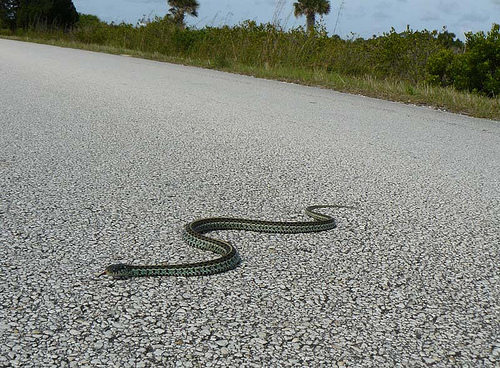
\includegraphics[trim={36mm 10mm 32mm 10mm},clip, width=\sizeP\textwidth]{fig/select/ILSVRC2012_val_00000006.JPEG}&
	\fig[\sizeS]{select/ILSVRC2012_val_00000006JPEG_vgg_GradCAM_vis.png} &
	\fig[\sizeS]{select/ILSVRC2012_val_00000006JPEG_vgg_GradCAMPlusPlus_vis.png} &
	\fig[\sizeS]{select/ILSVRC2012_val_00000006JPEG_vgg_ScoreCAM_vis.png} &
	\fig[\sizeS]{select/ILSVRC2012_val_00000006JPEG_vgg_AblationCAM_vis.png} &
	\fig[\sizeS]{select/ILSVRC2012_val_00000006JPEG_vgg_XGradCAM_vis.png} &
	\fig[\sizeS]{select/ILSVRC2012_val_00000006JPEG_vgg_versionP0_vis.png}  \\

	\rotatebox{90}{~Tricycle} &
	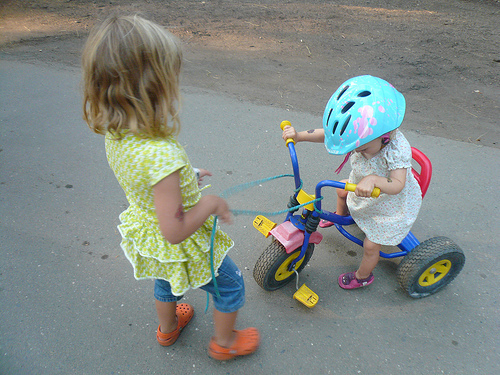
\includegraphics[trim={28mm 10mm 39mm 10mm},clip, width=\sizeP\textwidth]{fig/select/ILSVRC2012_val_00000069.JPEG}&
	\fig[\sizeS]{select/ILSVRC2012_val_00000069JPEG_vgg_GradCAM_vis.png} &
	\fig[\sizeS]{select/ILSVRC2012_val_00000069JPEG_vgg_GradCAMPlusPlus_vis.png} &
	\fig[\sizeS]{select/ILSVRC2012_val_00000069JPEG_vgg_ScoreCAM_vis.png} &
	\fig[\sizeS]{select/ILSVRC2012_val_00000069JPEG_vgg_AblationCAM_vis.png} &
	\fig[\sizeS]{select/ILSVRC2012_val_00000069JPEG_vgg_XGradCAM_vis.png} &
	\fig[\sizeS]{select/ILSVRC2012_val_00000069JPEG_vgg_versionP0_vis.png}  \\

	\rotatebox{90}{~Pneumonia} &
	\fig[\sizeS]{medical/chest_VGG16_GradCAM_1_img.png} &
	\fig[\sizeS]{medical/chest_VGG16_GradCAM_1_vis.png} &
	\fig[\sizeS]{medical/chest_VGG16_GradCAMPlusPlus_1_vis.png} &
	\fig[\sizeS]{medical/chest_VGG16_ScoreCAM_1_vis.png} &
	\fig[\sizeS]{medical/chest_VGG16_AblationCAM_1_vis.png} &
	\fig[\sizeS]{medical/chest_VGG16_XGradCAM_1_vis.png} &
	\fig[\sizeS]{medical/chest_VGG16_OptCAM_plain_1_vis.png}  \\


	\rotatebox{90}{~Pylorus} &
	\fig[\sizeS]{medical/kvasir_Resnet50_GradCAM_3_img.png} &
	\fig[\sizeS]{medical/kvasir_VGG16_GradCAM_3_vis.png} &
	\fig[\sizeS]{medical/kvasir_VGG16_GradCAMPlusPlus_3_vis.png} &
	\fig[\sizeS]{medical/kvasir_VGG16_ScoreCAM_3_vis.png} &
	\fig[\sizeS]{medical/kvasir_VGG16_AblationCAM_3_vis.png} &
	\fig[\sizeS]{medical/kvasir_VGG16_XGradCAM_3_vis.png} &
	\fig[\sizeS]{medical/kvasir_VGG16_OptCAM_plain_3_vis.png}  \\

\end{tabular}
\caption{Saliency maps obtained by different methods for ImageNet (top two rows), Chest X-ray (row 3) and Kvasir (row 4) with VGG. \iavr{Ground truth class shown on the left of the input image.}}
\label{fig:vis-in-chest-n-kvasir-resnet}
% \vspace{-0.4cm}
\end{figure*}
%------------------------------------------------------------------------------

\paragraph{Visualization}

\autoref{fig:vis-in-chest-n-kvasir-resnet} illustrates saliency map examples from ImageNet, Chest X-ray and Kvasir datasets. Opti-CAM saliency map is in general more spread out. This better highlights full objects, multiple instances or \iavr{background context, which may be taken into account by the model. On Chest X-ray, Opti-CAM and Score-CAM are the only methods that capture the chest, while all others focus on image corners.} More examples on datasets and networks \redred{as well as quantitative evaluation on medical data} are given in the supplementary material.

\subsection{Object localization}

\iavr{Localization metrics are used to measure the precision of saliency maps relative to ground truth bounding boxes of the foreground object of interest. These metrics originate from weakly supervised localization (WSOL). However, the objectives of WSOL and explaining the decision of a DNN are not necessarily aligned, since context may play an important role in the decision~\cite{shetty2019not, rao2022towards}.

To investigate the relative importance of the object and its context, we measure classification metrics} when using the bounding box $B$ itself as a saliency map as well as its complement $I \setminus B$, where $I$ is the image. We also evaluate the \modify{intersection $B \cap S$} of the saliency map $S$ with the bounding box and with its complement ($S \setminus B$).

As shown in \autoref{tab:localization}, the ground truth region of the object is not the only one responsible for the network decision. For example, the bounding box fails both when used as a saliency map itself and when combined with any saliency map, by harming all classification metrics. Even the complement is more effective than the bounding box itself, either alone or when combined. These findings support the hypothesis that localization metrics based on the ground truth bounding box are not necessarily appropriate for evaluating explanations of network decisions. Classification metrics are clearly more appropriate in this sense.

Nevertheless, we report localization metrics in the supplementary material. In summary, although its saliency maps are more spread out, Opti-CAM outperforms other methods on a number of metrics.

%------------------------------------------------------------------------------
\begin{table}[t]
\footnotesize
\centering
\setlength{\tabcolsep}{4pt}
\renewcommand{\arraystretch}{0.8}
\begin{tabular}{lccc|ccc|ccc} \toprule
\mr{2}{\Th{Method}}                            & \mc{3}{\Th{$\AD\!\downarrow$}} & \mc{3}{\Th{$\AG\!\uparrow$}}& \mc{3}{\Th{$\AI\!\uparrow$}} \\ \cmidrule{2-10}
                                               & {$S$} & {$B \!\cap\! S$} & {$S \!\setminus\! B$} & {$S$} & {$B \!\cap\! S$} & {$S \!\setminus\! B$}& {$S$} & {$B \!\cap\! S$} & {$S \!\setminus\! B$} \\ \midrule
$S \defn B$                                    & 67.2 &   -- &   -- &  2.3 &   -- &   -- &  9.2 &   -- &   -- \\
$S \defn I \setminus B$                        & 44.0 &   -- &   -- &  2.8 &   -- &   -- & 16.3 &   -- &   -- \\ \midrule
Fake-CAM~\citep{poppi2021revisiting}           &  0.5 & 67.2 & 44.1 &  0.7 &  2.3 &  2.8 & 42.0 &  9.2 & 18.9 \\ \midrule
Grad-CAM~\citep{selvaraju2017grad}             & 15.0 & 72.6 & 52.1 & 15.3 &  1.8 &  6.0 & 40.4 &  8.4 & 19.4 \\
Grad-CAM++~\cite{chattopadhay2018grad}         & 16.5 & 72.9 & 53.1 & 10.6 &  1.6 &  4.1 & 35.2 &  7.3 & 17.1 \\
Score-CAM~\citep{wang2020score}                & 12.5 & 71.5 & 50.5 & 16.1 &  2.2 &  6.3 & 42.5 &  8.6 & 20.8 \\
Ablation-CAM~\citep{ramaswamy2020ablation}     & 15.1 & 72.8 & 52.1 & 13.5 &  1.7 &  5.6 & 39.9 &  7.8 & 19.0 \\
XGrad-CAM~\citep{fu2020axiom}                  & 14.3 & 72.6 & 51.4 & 15.1 &  1.8 &  6.0 & 42.1 &  8.0 & 20.1 \\
Layer-CAM~\citep{jiang2021layercam}            & 49.2 & 84.2 & 74.4 &  2.7 &  0.4 &  1.2 & 12.7 &  4.4 &  7.3 \\
ExPerturbation~\citep{fong2019understanding}   & 43.8 & 81.6 & 71.0 &  7.1 &  1.4 &  3.2 & 18.9 &  5.6 & 11.1 \\
\rowcolor{cyan!10}
Opti-CAM (ours)                                & \tb{1.4} & \tb{62.5} & \tb{34.8} & \tb{66.3} & \tb{8.7} & \tb{25.8} & \tb{92.5} & \tb{18.6} & \tb{47.1} \\ \bottomrule
\end{tabular}
\caption{\textbf{Bounding box} study. Classification metrics on ImageNet validation set using VGG16. $B$: ground-truth box used by localization metrics; $I$: entire image; $S$: saliency map. $\AD$/$\AI$: average drop/increase~\citep{chattopadhay2018grad}; $\AG$: average gain (ours); $\downarrow$ / $\uparrow$: lower / higher is better; bold: best, excluding Fake-CAM.}
\label{tab:localization}
% \vspace{-0.2cm}
\end{table}
%------------------------------------------------------------------------------

%--------------------------------------------------------------------------------------------------
\section{Ablation study}
\label{sec:ablation}

We perform an ablation study of different choices of the objective function~\eq{obj} and 
normalization~\eq{norm} of the saliency map. %\redred{More choices of~\eq{obj}, layer $\ell$, number 
%of iterations and learning rates, selector function $g_c$ and initialization of $\vw$ are studied 
%in the supplementary material.}

\paragraph{Normalization function}
For normalization function $n$~\eq{obj}, we investigate three choices:
\begin{align}
	\textrm{range}: \quad & n(A) \defn \textstyle \frac{A-\min A}{\max A-\min A}\label{eq:n-rng}\\
	\textrm{maximum}: \quad & n(A) \defn \textstyle \frac{A}{\max A}\label{eq:n-max}\\
 	\textrm{sigmoid}: \quad & n(a_{ij}) \defn \frac{1}{1+e^{-a_{ij}}}\label{eq:n-sig},
\end{align}
where $a_{ij}$ is element $(i,j)$ of matrix $A$. The default is~\eq{n-rng}, normalizing by the 
range of values in the saliency map, as in Score-CAM~\eq{norm}; while~\eq{n-max} normalizes by the 
maximum value and~\eq{n-sig} by the sigmoid function element-wise.

%--------------------------------------------------------------------------------------------------

\paragraph{Objective function}

We refer to the default definition of $F^c_\ell$~\eq{obj} as \Fdef because it maximizes the logit 
for the masked image.
We also consider an alternative definition of objective function $F^c_\ell$, which encourages the 
masked version to preserve the prediction of original image:
\begin{equation}
	F^c_\ell(\vx; \vu) \defn -\abs{g_c(f(\vx)) - g_c(f(\vx \odot n(\up(S_\ell(\vx; \vu)))))}.
\label{eq:ref}
\end{equation}
This function is named \Fref as it minimizes the difference of logits between the masked and the 
original image.

%--------------------------------------------------------------------------------------------------

\paragraph{Results}

\autoref{tab:ablate} shows classification metrics for the different choices of Opti-CAM, as well as 
comparison to other methods for reference, for the small subset of ImageNet validation set.\\
% \redred{A similar ablation table with localization metrics is available in supplementary material.}

\noindent We observe that the choice of normalization function has little effect overall and Sigmoid 
offers lower performance. Note that the minimum value of saliency maps is often zero or close to 
zero: \emph{Saliency maps are non-negative as convex combinations of non-negative feature maps
~\eq{v-sal}.} In contrast, the choice of loss function has more impact on performance, and we 
observe that \Fdef~\eq{obj} is superior on all cases.

\newcommand{\ob}[1]{\textcolor{brown}{\tb{#1}}}
\newcommand{\ab}[1]{\textcolor{blue}{\tb{#1}}}
\begin{table}[t]
\centering
\footnotesize
\setlength{\tabcolsep}{4pt}
\renewcommand{\arraystretch}{0.8}
\begin{tabular}{lccrrrrr} \toprule
{\Th{Method}} & {$F^c_\ell$} & {$n$} & {$\AD\!\downarrow$}& {$\AG\!\uparrow$} & {$\AI\!\uparrow$}\\ \midrule
Fake-CAM       & & & 0.5  &  0.7 & 42.1 \\
\midrule
Grad-CAM       & & & 15.0 & 15.3 & 40.4 \\
Grad-CAM++     & & & 16.5 & 10.6 & 35.2  \\
Score-CAM      & & & 12.5 & 16.1 & 42.6  \\
Ablation-CAM   & & & 15.1 & 13.5 & 39.9  \\
XGrad-CAM      & & & 14.3 & 15.1 & 42.1  \\
Layer-CAM      & & & 49.2 &  2.7 & 12.7  \\
ExPerturbation & & & 43.8 &  7.1 &  18.9  \\
\midrule
\mr{2}{Opti-CAM} & \Fdef~\eq{obj}  & Range~\eq{n-rng}   & \tb{1.4} & \tb{66.3} & \tb{92.5} \\
	& \Fref~\eq{ref}  & Range~\eq{n-rng}   &     7.1  &     18.5  &     54.9  \\ \midrule
\mr{2}{Opti-CAM} & \Fdef~\eq{obj}  & Max~\eq{n-max}     &     1.6  &     66.2  &     90.3  \\
    & \Fref~\eq{ref}  & Max~\eq{n-max}     &     6.8  &     17.8  &     54.5  \\ \midrule
\mr{2}{Opti-CAM} & \Fdef~\eq{obj}  & Sigmoid~\eq{n-sig} &     5.0  &     18.3  &     57.5  \\
    & \Fref~\eq{ref}  & Sigmoid~\eq{n-sig} &     6.5  &     10.0  &     45.3  \\ \bottomrule
\end{tabular}
\caption{\textbf{Ablation study} using VGG16 on 1000 images of ImageNet validation set. $\AD$/$\AI$: 
average drop/increase \autocite{chattopadhay2018grad}; $\AG$: average gain (ours); $\downarrow$ / 
$\uparrow$: lower / higher is better; bold: best, excluding Fake-CAM.}
\label{tab:ablate}
% \vspace{-0.2cm}
\end{table}
%------------------------------------------------------------------------------

%------------------------------------------------------------------------------
%\pgfplotstableread{fig/eval/plain_ai.dat}{\plotAI}
%\pgfplotstableread{fig/eval/plain_ad.dat}{\plotAD}
%\pgfplotstableread{fig/eval/plain_ag.dat}{\plotAG}
%------------------------------------------------------------------------------

%--------------------------------------------------------------------------------------------------
\section{Conclusion}
\label{sec:ca_conclusion}
In this chapter we observe that attention-based pooling in transformers is the same as 
forming a class agnostic CAM-based saliency map. This map is used to mask the features before 
global average pooling, much like we mask inputs to confirm that the prediction is due to a certain 
object. This observation establishes that transformers have a built-in CAM-based interpretability 
mechanism and allows us to design a similar mechanism for convolutional networks. Masking in feature 
space is much more efficient than in the input space as it requires only one forward pass, although 
of course it is not equivalent because of interactions within the network.\\

\noindent Although the saliency maps obtained with our \Ours are not very different from those 
obtained with \gap, our approach improves a number of CAM-based interpretability methods on a number 
of convolutional networks according to most interpretability metrics, while preserving classification 
accuracy. By doing so, it also enhances the differences in performance between interpretability methods, 
facilitating their evaluation. Further study may be needed to improve the differentiation of saliency 
maps themselves, to possibly make a class specific representation more competitive and to apply the 
approach to more architectures, including transformers.

\section*{Acknowledgements}
This publication has received funding from the Excellence Initiative of Aix-Marseille Universite - A*Midex, a French “Investissements d’Avenir programme” (AMX-21-IET-017), and the UnLIR ANR project (ANR-19-CE23-0009). Part of this work was performed using HPC resources from GENCI-IDRIS (Grant 2020-AD011013110).

\clearpage

% \title{Supplementary material for \\
% ``Opti-CAM: Optimizing saliency maps for interpretability''}

% % COMMENT OUT \maketitle FROM main.tex FOR \maketitle TO WORK HERE
% \maketitle

% PAGE NUMBER SET TO 1
% \setcounter{page}{1}

% START APPENDIX
\appendix


% NUMBERING
\renewcommand{\theequation}{A\arabic{equation}}
\renewcommand{\thetable}{A\arabic{table}}
\renewcommand{\thefigure}{A\arabic{figure}}

%------------------------------------------------------------------------------

\section*{Appendices}

Implementation details are provided in \autoref{sec:details}. We provide results on more classification metrics in \autoref{sec:cla-metrics}. In \autoref{sec:loc-metrics}, we define localization metrics and provide corresponding results. We provide results on medical data in \autoref{sec:medical}. We then provide more ablation results in \autoref{sec:more-ablation}, sanity check in \autoref{sec:sanity-check}, and results without input image normalization in \autoref{sec:without-norm}. 
% Finally, we provide additional visualizations in \autoref{sec:more-vis}.

%------------------------------------------------------------------------------

\section{Implementation details}
\label{sec:details}

All input images are resized to $224 \times 224 \times 3$. To optimize the saliency map with Opti-CAM~\eq{opt}, we use the Adam~\citep{kingma2014adam} optimizer with learning rate $0.1$ by default, setting the maximum number of iterations to $100$ and stopping early when the change in loss is less than $10^{-10}$. For VGG16, we generate the saliency map~\eq{v-sal} from the feature maps of the last convolutional layer before max pooling by default, \ie convolutional layer 3 of block 5. For ResNet50, we choose the last convolutional layer by default, \ie convolutional layer 3 of bottleneck 2 of block 4. For ViT and DeiT, we choose the last self-attention block by default, \ie layer normalization of self-attention block 12. Ablations concerning the layer $\ell$ and the convergence of Opti-CAM are included in \autoref{sec:more-ablation}.

%------------------------------------------------------------------------------

\section{Classification metrics}
\label{sec:cla-metrics}

Classification metrics measure the effect on classification performance of masking (element-wise multiplying) the input image by the saliency map. We have used $\AD$, $\AG$ and $\AI$ in the main paper. Here we discuss Insertion/Deletion~\citep{petsiuk2018rise}, providing results and discussing failure cases for Opti-CAM.

\subsection{Insertion/Deletion}

\paragraph{Definition}

Insertion/Deletion~\citep{petsiuk2018rise} are based on the probability $p^{c_p}_i$ for the predicted class $c_p$ as pixels are ``inserted'' or ``deleted'' from image $\vx_i$, averaged over the number of pixels and over all images in the test set.

\emph{Deletion} measures the decrease in the probability of class $c_p$ when removing pixels one by one in decreasing order of saliency, where removal is taken as setting the value to zero; lower is better.

\emph{Insertion}, by contrast, measures the increase in the probability of class $c_p$ when adding pixels, again by decreasing order of saliency. In this case, we begin with a version of the image that is distorted by Gaussian blur and then addition is taken as setting the value of the pixel according to the original image. Higher is better.

\paragraph{Results}

The experimental results are shown in \autoref{tab:imagenet_cnn_hihd} for CNNs and transformers. ExPerturbation~\citep{fong2019understanding} is expected to perform best in insertion because its optimization objective is very similar to this evaluation metric, using blurring for masked regions. However, ExPerturbation~\citep{fong2019understanding}  only performs best on ResNet50. TIBAV~\cite{chefer2021transformer}, which is designed for transformers, outperforms the other methods on DeiT and ViT. According to the results of Insertion/Deletion, Opti-CAM has low performance but there is no clear winner on either CNNs or transformers.

To further understand the behavior of Opti-CAM, we investigate in \autoref{fig:hihd} examples where Score-CAM succeeds (insertion score greater than $90$ and deletion score less than $10$) and Opti-CAM fails (insertion score less than $70$ and deletion score greater than $15$). Compared with Score-CAM, the saliency maps obtained by Opti-CAM are more spread out and highlight several parts of the object and background context. In most of the cases, Opti-CAM fails I/D because it not only finds the object but also attaches importance to the background.

We argue that this is not a failure. As our localization experiment in \autoref{tab:localization} indicates, the background is useful in discriminating a class. Often, the network recognizes the background better than the object itself. For example, a gas pump is likely to be seen with a truck, and a hare is often seen on grass. Several parts of the object are highlighted by Opti-CAM for the worm fence, terrier dog, hare, and manhole cover. Finally, several instances of spaniel dog are found by Opti-CAM.

Insertion/Deletion include 224 steps of binarization, with a set of 224 pixels being inserted/deleted at each step. If these pixels are all inserted over a single small area, the effect on the classifier is more immediate than when sparsely inserting pixels over multiple areas. The same observation holds for deletion. By contrast, Opti-CAM attempts to find regions that contribute to the classification as a whole. There is no guarantee that those regions are effective when used in isolation.

%------------------------------------------------------------------------------
\begin{table}
\centering
\footnotesize
\setlength{\tabcolsep}{8pt}
\renewcommand{\arraystretch}{0.8}
\begin{tabular}{lrr rr rr rr} \toprule
\mr{2}{\Th{Method}} & \mc{2}{\Th{ResNet50}} & \mc{2}{\Th{VGG16}} & \mc{2}{\Th{ViT-B}}& \mc{2}{\Th{DeiT-B}} \\ \cmidrule{2-9}
                    & {{$\I\!\uparrow$}} & {{$\D\!\downarrow$}}& {{$\I\!\uparrow$}} & {{$\D\!\downarrow$}} & {{$\I\!\uparrow$}} & {{$\D\!\downarrow$}}& {{$\I\!\uparrow$}} & {{$\D\!\downarrow$}}\\ \midrule
Fake-CAM~\citep{poppi2021revisiting}&50.7&28.1&46.1&26.9&57.4&33.3&57.5&34.2\\\midrule
Grad-CAM~\citep{selvaraju2017grad}          &66.3&14.7&\tb{64.1}&11.6&62.9&19.8&61.8&17.5\\
Grad-CAM++~\cite{chattopadhay2018grad}     &66.0&14.7&62.9&12.2&56.7&29.3&60.5&21.9\\
Score-CAM~\citep{wang2020score}         &65.7&16.3&62.5&12.1&\tb{66.5}&15.1 &60.6&24.4\\
XGrad-CAM~\citep{fu2020axiom}             &66.3&14.7&\tb{64.1}&11.7&55.6&26.5  &55.2&31.1\\
%\midrule
Layer-CAM~\citep{jiang2021layercam}&67.0&\tb{14.2}&58.3&\tb{6.4}&62.9&14.6 &61.6&21.2\\
ExPerturbation~\citep{fong2019understanding}&\tb{70.7}&15.0&61.1&15.0&64.4&18.4&62.1&27.0\\
Ablation-CAM~\citep{ramaswamy2020ablation} &65.9&14.6&63.8&11.4&-&-&-&-\\
RawAtt~\citep{dosovitskiy2020image}   &-&-&-&-&62.2&17.9 &56.3&29.3\\
Rollout~\citep{abnar2020quantifying}   &-&-&-&-&64.8&15.2 &56.7&32.8\\
TIBAV~\cite{chefer2021transformer}    &-&-&-&-&66.1&\tb{14.1} &\tb{63.7}&\tb{16.3}\\
\rowcolor{cyan!10}
Opti-CAM (ours)                        &62.0&19.7&59.2&11.0 &60.5&22.0  &59.2&22.8\\
\bottomrule
\end{tabular}
% \vspace{6pt}
\caption{
I/D: insertion/deletion~\citep{petsiuk2018rise} scores on ImageNet validation set; $\downarrow$ / $\uparrow$: lower / higher is better.}% Bold: best, excluding Fake-CAM.}
\label{tab:imagenet_cnn_hihd}
\end{table}
%------------------------------------------------------------------------------

% %------------------------------------------------------------------------------
% \begin{table}
% \centering
% \footnotesize
% \setlength{\tabcolsep}{8pt}
% \renewcommand{\arraystretch}{0.8}
% \begin{tabular}{lrr rr} \toprule
% \mr{2}{\Th{Method}} & \mc{2}{\Th{ViT-B}}& \mc{2}{\Th{DeiT-B}}  \\ \cmidrule{2-5}
%                     & {{$\I\!\uparrow$}} & {{$\D\!\downarrow$}}&   {{$\I\!\uparrow$}} & {{$\D\!\downarrow$}} \\ \midrule
% Fake-CAM~\citep{poppi2021revisiting}&57.4&33.3&57.5&34.2\\\midrule
% Grad-CAM~\citep{selvaraju2017grad}          &62.9&19.8&61.8&17.5\\
% Grad-CAM++~\cite{chattopadhay2018grad}     &56.7&29.3&60.5&21.9\\
% Score-CAM~\citep{wang2020score}        &\tb{66.5}&15.1 &60.6&24.4\\
% XGrad-CAM~\citep{fu2020axiom}           &55.6&26.5  &55.2&31.1\\
% Layer-CAM~\citep{jiang2021layercam}&62.9&14.6 &61.6&21.2\\
% ExPerturbation~\citep{fong2019understanding}&64.4&18.4&62.1&27.0\\
% RawAtt~\citep{dosovitskiy2020image}   &62.2&17.9 &56.3&29.3\\
% Rollout~\citep{abnar2020quantifying}   &64.8&15.2 &56.7&32.8\\
% TIBAV~\cite{chefer2021transformer}    &66.1&\tb{14.1} &\tb{63.7}&\tb{16.3}\\
% \rowcolor{cyan!10}
% Opti-CAM (ours)                      &60.5&22.0  &59.2&22.8\\


% \bottomrule
% \end{tabular}
% % \vspace{6pt}
% \caption{
% \emph{I/D: insertion/deletion~\citep{petsiuk2018rise}} scores on ImageNet validation set; $\downarrow$ / $\uparrow$: lower / higher is better.}% Bold: best, excluding Fake-CAM.}
% \label{tab:imagenet-trans-hihd}
% \end{table}
% %------------------------------------------------------------------------------

%------------------------------------------------------------------------------
\begin{figure}[thpb]
\newcommand{\sizeP}{.12}
\newcommand{\sizeS}{.12}
\newcommand{\hh}{.175\textwidth}
\newcommand{\ww}{.200\textwidth}
\tiny
\centering
\setlength{\tabcolsep}{3pt}
\begin{tabular}{cccccc}
\centering
Original & Opti-CAM & Score-CAM & Original & Opti-CAM & Score-CAM\\
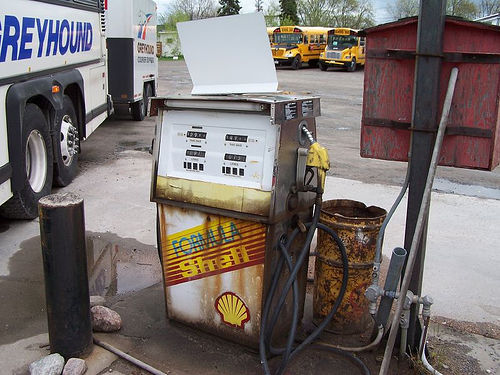
\includegraphics[trim={28mm 8mm 28mm 8mm},clip, width=\sizeP\textwidth]{fig/eval/hihd/ILSVRC2012_val_00045353.JPEG}
&
\fig[\sizeS]{eval/hihd/ILSVRC2012_val_00045353JPEG_smap_opticam.png} 
&  
\fig[\sizeS]{eval/hihd/ILSVRC2012_val_00045353JPEG_smap_scorecam.png} &
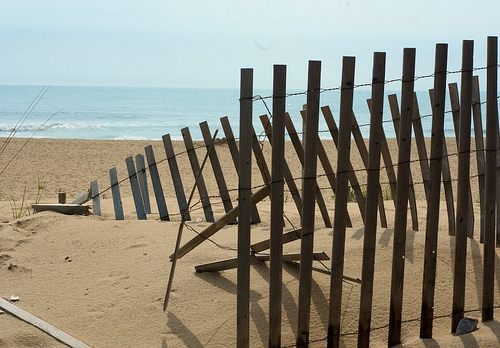
\includegraphics[trim={32mm 14mm 36mm 1mm},clip, width=\sizeP\textwidth]{fig/eval/hihd/ILSVRC2012_val_00041066.JPEG}
&
\fig[\sizeS]{eval/hihd/ILSVRC2012_val_00041066JPEG_smap_opticam.png} 
&          
\fig[\sizeS]{eval/hihd/ILSVRC2012_val_00041066JPEG_smap_scorecam.png} \\
gas pump&I$\uparrow$:66.3, D$\downarrow$:19.4&I$\uparrow$:94.2, D$\downarrow$:9.4&
worm fence&I$\uparrow$:69.7, D$\downarrow$:16.8&I$\uparrow$:91.9, D$\downarrow$:4.4\\
&AG$\uparrow$:100.0, AD$\downarrow$:0.0&AG$\uparrow$:0.0, AD$\downarrow$:0.0&
&AG$\uparrow$:73.2, AD$\downarrow$:0.0&AG$\uparrow$:0.0, AD$\downarrow$:28.8\\
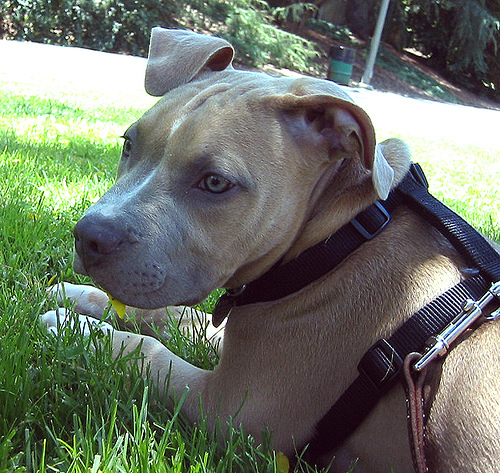
\includegraphics[trim={10mm 14mm 10mm 4mm},clip, width=\sizeP\textwidth]{fig/eval/hihd/ILSVRC2012_val_00040673.JPEG}
&        
\fig[\sizeS]{eval/hihd/ILSVRC2012_val_00040673JPEG_smap_opticam.png} 
&
\fig[\sizeS]{eval/hihd/ILSVRC2012_val_00040673JPEG_smap_scorecam.png} &
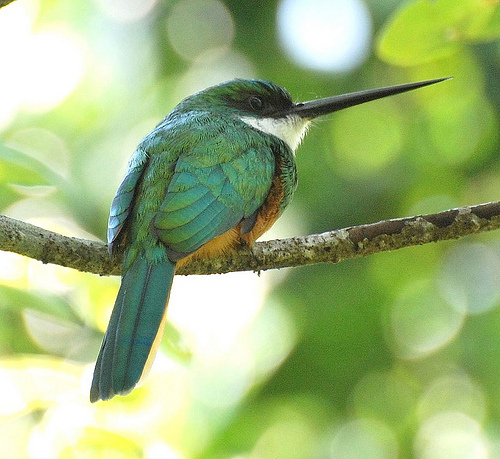
\includegraphics[trim={18mm 6mm 10mm 12mm},clip, width=\sizeP\textwidth]{fig/eval/hihd/ILSVRC2012_val_00030507.JPEG}
&
\fig[\sizeS]{eval/hihd/ILSVRC2012_val_00030507JPEG_smap_opticam.png} 
&                
\fig[\sizeS]{eval/hihd/ILSVRC2012_val_00030507JPEG_smap_scorecam.png} \\
staffordshire terrier&I$\uparrow$:62.1, D$\downarrow$:32.2&I$\uparrow$:93.4, D$\downarrow$:8.2&
jacamar&I$\uparrow$:66.3, D$\downarrow$:17.3&I$\uparrow$:94.6, D$\downarrow$:9.9\\
&AG$\uparrow$:41.3, AD$\downarrow$:0.0&AG$\uparrow$:0.0, AD$\downarrow$:0.3&
&AG$\uparrow$:91.4, AD$\downarrow$:0.0&AG$\uparrow$:56.5, AD$\downarrow$:0.0\\
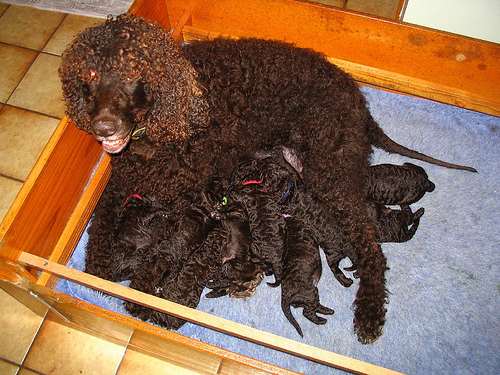
\includegraphics[trim={6mm 1mm 6mm 1mm},clip, width=\sizeP\textwidth]{fig/eval/hihd/ILSVRC2012_val_00029237.JPEG}
&
\fig[\sizeS]{eval/hihd/ILSVRC2012_val_00029237JPEG_smap_opticam.png} 
&     
\fig[\sizeS]{eval/hihd/ILSVRC2012_val_00029237JPEG_smap_scorecam.png} &
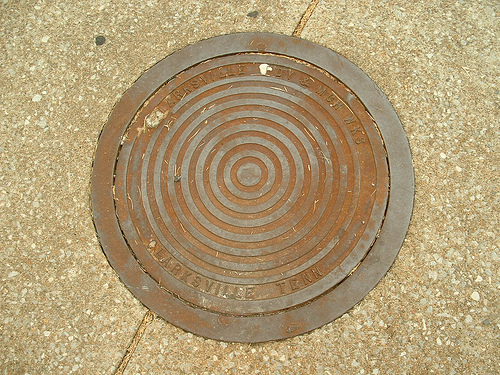
\includegraphics[trim={28mm 5mm 22mm 5mm},clip, width=\sizeP\textwidth]{fig/eval/hihd/ILSVRC2012_val_00005077.JPEG}
&
\fig[\sizeS]{eval/hihd/ILSVRC2012_val_00005077JPEG_smap_opticam.png} 
&          
\fig[\sizeS]{eval/hihd/ILSVRC2012_val_00005077JPEG_smap_scorecam.png} \\
Irish water spaniel&I$\uparrow$:52.6, D$\downarrow$:18.8&I$\uparrow$:90.5, D$\downarrow$:8.6&
manhole cover&I$\uparrow$:65.8, D$\downarrow$:29.6&I$\uparrow$92.7, D$\downarrow$:9.1\\
&AG$\uparrow$:86.4, AD$\downarrow$:0.0&AG$\uparrow$:65.1, AD$\downarrow$:0.0&
&AG$\uparrow$:24.0, AD$\downarrow$:0.0&AG$\uparrow$:0.0, AD$\downarrow$:59.9\\
% 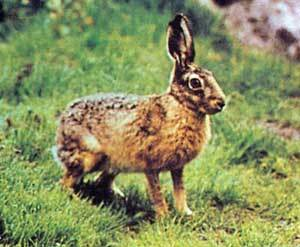
\includegraphics[trim={12mm 5mm 12mm 5mm},clip, width=\sizeP\textwidth]{fig/eval/hihd/ILSVRC2012_val_00003602.JPEG}
% &              
% \fig[\sizeS]{eval/hihd/ILSVRC2012_val_00003602JPEG_smap_opticam.png} 
% & 
% \fig[\sizeS]{eval/hihd/ILSVRC2012_val_00003602JPEG_smap_scorecam.png} \\
% hare&I$\uparrow$:61.3, D$\downarrow$:21.2&I$\uparrow$91.3, D$\downarrow$:8.9\\
% &AG$\uparrow$:93.7, AD$\downarrow$:0.0&AG$\uparrow$:0.0, AD$\downarrow$:0.6\\
\end{tabular}
\caption{Failure examples of Opti-CAM regarding insertion/deletion.}
\label{fig:hihd}
\end{figure}
%------------------------------------------------------------------------------

%------------------------------------------------------------------------------

\modify{

\subsection{More metrics}
In this section, we show additional metrics including AOPC~\citep{samek2016evaluating}, Max-Sensitivity~\citep{yeh2019fidelity} and ADCC~\citep{poppi2021revisiting}.
%
% \subsubsection{Definitions}
%
% \paragraph{AOPC.} Similar to \emph{Deletion}, AOPC considers removing the most relevant region first. After sorting the value of each position in saliency maps, instead of replacing them one by one with zero value, AOPC removes all pixels in a $9 \times 9$ neighborhood around the position by randomly sampled values from a uniform distribution. Then AOPC calculates the difference between the probability of the images $\vx$ and the probability of regions "deleted" from images $\vx$ and averages over the number of regions and over all images in the test set. Thus a larger value of AOPC implies the most sensitive regions are ranked first by saliency maps. 
%
% \paragraph{Max-Sensitvity (MS).} Given a network $f$, a function $S(\vx)$ to generate a saliency map for input images $\vx$ and a given input neighborhood radius $\epsilon$, then the max-sensitivity (MS) is define as
% \begin{equation}
%     MS \defn \max_{\|\vy-\vx\| \leq \epsilon} \| S(\vy) - S(\vx) \|.
% \end{equation}
%
% \paragraph{ADCC.} ADCC is a combination of three scores, \ie coherency (CH), complexity (CP), and Average Drop (AD). Let $S(\vx)$ denote the saliency maps for images $\vx$, $PCC(\vx,\vy)$ denote the function to calculate Pearson Correlation Coefficient between $\vx$ and $\vy$ and $\delta_{\vx}$ denote the standard deviation of $\vx$, the ADCC is define as
% \begin{align}
%     ADCC \defn & 3 ( \frac{1}{CH} + \frac{1}{1-CP} + \frac{1}{1-AD})^{-1}, \\
%     CH \defn & \frac{PCC(S(\vx),S(\vx \odot S(\vx)))}{\delta_{S(\vx)}\delta_{S(\vx \odot S(\vx))}},\\
%     CP \defn & \| S(\vx)\|_1.
% \end{align}
%
% \subsubsection{Resluts}
%
We use the code and suggested parameters of package Quantus\footnote{\url{https://github.com/understandable-machine-intelligence-lab/Quantus}} to measure AOPC and MS. In particular, patch size $14$ and number of evaluation regions $10$ for AOPC; lower bound $0.2$ and number of samples $10$ for MS.
For ADCC, we use the official code\footnote{\url{https://github.com/aimagelab/ADCC?fbclid=IwAR0YK_93lxp4pZQnt34SlA9aeNCLRX8m0u8yTZPxbTXi80qiyhTiqxWaQ7o}}.
We evaluate these metrics on ImageNet validation set using ResNet50 and VGG16. The results are reported in \autoref{tab:more-metrics-asked}. Since AOPC shares the same philosophy as I/D, it is not a surprise that Opti-CAM has poor performance on AOPC. Opti-CAM achieves the best performance on MS.
}

\begin{table}[]
\centering
\footnotesize
\setlength{\tabcolsep}{4pt}
\begin{tabular}{lrrr rrr} \toprule
\mr{2}{\Th{Method}} & \mc{3}{\Th{ResNet50}} & \mc{3}{\Th{VGG16}}  \\ \cmidrule{2-7}
                    & {{$AOPC\uparrow$}} & {{$MS\downarrow$}}& {{$ADCC\downarrow$}} & {{$AOPC\uparrow$}} & {{$MS\downarrow$}}& {{$ADCC\downarrow$}}  \\ \midrule
Grad-CAM~\citep{selvaraju2017grad}         &11.7&1.05&74.3&13.1&1.10&73.7        \\
Grad-CAM++~\cite{chattopadhay2018grad}     &11.6&1.04&73.6&11.6&1.09&74.6          \\
Score-CAM~\citep{wang2020score}            &10.2&1.04&61.0&11.0&1.09&73.9             \\
XGrad-CAM~\citep{fu2020axiom}              &11.9&1.05&74.3&13.1&1.10&73.9           \\
Ablation-CAM~\citep{ramaswamy2020ablation} &11.1&1.04&71.5&12.5&1.10&75.5          \\
Layer-CAM~\citep{jiang2021layercam} &\tb{13.0}&1.22&61.1&\tb{13.3}&1.25&51.7 \\
ExPerturbation~\citep{fong2019understanding}  &12.0&1.07&\tb{26.0}&11.2&1.09&\tb{42.8}  \\
\rowcolor{cyan!10}
Opti-CAM (ours)                            &6.3&\tb{1.03}&65.5&8.9&\tb{1.06}&70.0        \\ \bottomrule

    \end{tabular}
    \caption{\modify{\emph{AOPC/MS/ADCC} scores on ImageNet validation set; $\downarrow$ / $\uparrow$: lower / higher is better.}}
    \label{tab:more-metrics-asked}
\end{table}

% \begin{table}[]
% \centering
% \footnotesize
% \setlength{\tabcolsep}{4pt}
% \begin{tabular}{lrrr rrr rrr rrr} \toprule
% \mr{2}{\Th{Method}} & \mc{3}{\Th{ResNet50}} & \mc{3}{\Th{VGG16}} & \mc{3}{\Th{ViT-B}}& \mc{3}{\Th{DeiT-B}} \\ \cmidrule{2-13}
%                     & {{$AOPC\uparrow$}} & {{$MS\downarrow$}}& {{$ADCC\downarrow$}} & {{$AOPC\uparrow$}} & {{$MS\downarrow$}}& {{$ADCC\downarrow$}} & {{$AOPC\uparrow$}} & {{$MS\downarrow$}}& {{$ADCC\downarrow$}}& {{$AOPC\uparrow$}} & {{$MS\downarrow$}}& {{$ADCC\downarrow$}} \\ \midrule
% Grad-CAM~\citep{selvaraju2017grad}         &13.0&1.05&75.8&13.1&1.11&73.7     &&1.49&&&&       \\
% Grad-CAM++~\cite{chattopadhay2018grad}     &9.2&1.04&74.4&11.6&1.09&74.6     &&1.70&&&&       \\
% Score-CAM~\citep{wang2020score}            &11.3&1.04&&11.0&1.09&73.9     &&1.25&&&&          \\
% XGrad-CAM~\citep{fu2020axiom}              &13.2&1.05&&13.1&1.10&     &&1.49&&&&         \\
% Ablation-CAM~\citep{ramaswamy2020ablation} &12.4&1.04&&12.5&1.10&     &-&-&-&-&-&-        \\
% Layer-CAM~\citep{jiang2021layercam} &16.6&1.22&&13.3&1.25& &-&-&-&-&-&-\\
% ExPerturbation~\citep{fong2019understanding}  &14.5&1.07&&11.2&1.09&  &-&-&-&-&-&-\\
% RawAtt~\citep{dosovitskiy2020image}  &-&-&-&-&-&-   &&1.89&&&&\\
% Rollout~\citep{abnar2020quantifying} &-&-&-&-&-&-   &&1.27&&&&\\
% TIBAV~\cite{chefer2021transformer}&-&-&-&-&-&-   &&1.60&&&&\\
% \rowcolor{cyan!10}
% Opti-CAM (ours)                            &6.6&1.03&&8.9&1.06&         &&1.09&&&&\\ \bottomrule

%     \end{tabular}
%     \caption{Caption}
%     \label{tab:more-metrics-asked}
% \end{table}





%------------------------------------------------------------------------------

\section{Localization metrics}
\label{sec:loc-metrics}

Several works measure the localization ability of saliency maps, using metrics from the \emph{weakly-supervised object localization} (WSOL) task. While we show in the main paper that localization of the object and classifier interpretability are not well aligned as tasks, we still provide localization results here. We use the \emph{official metric} (OM), \emph{localization error} (LE), \emph{pixel-wise $F_1$ score}, \emph{box accuracy} (BoxAcc)~\citep{choe2020evaluating}, standard pointing game (SP)~\cite{zhang2018top}, \emph{energy pointing game} (EP)~\citep{wang2020score} and \emph{saliency metric} (SM)~\citep{dabkowski2017real} on the ILSVRC2014\footnote{\url{https://www.image-net.org/challenges/LSVRC/2014/index\#}} dataset. The goal of these metrics is to compare the saliency maps with bounding boxes around the object of interest. For simplicity, we define these metrics for a single image; the reported results are averaged over all images of the test set.

\subsection{Definitions}

We are given the saliency map $S^c$ obtained from test image $\vx$ for ground truth class $c$. We denote by $S^c_{\vp}$ its value at pixel $\vp$. We binarize the saliency map by thresholding at its average value and we take the bounding box of the largest connected component of the resulting mask as the predicted bounding box $B_p$, represented as a set of pixels. We compare this box against the set of ground truth bounding boxes $\cB$, which typically contains 1 or 2 boxes of the same class $c$, or with their union $U = \cup \cB$, again represented as a set of pixels. We also compare the predicted class label $c_p$ with the ground truth label $c$. All metrics take values in $[0,1]$ and are expressed as percentages, except SM~\eq{sm}, which is unbounded.

\paragraph{Official Metric (OM)}

measures the maximum overlap of the predicted bounding box with any ground truth bounding box, requiring that the predicted class label is correct:
\begin{equation}
	\OM \defn 1 - \paren{\max_{B \in \cB} \iou(B, B_p)} \ind_{c_p = c},
\label{eq:om}
\end{equation}
where $\iou$ is intersection over union.
% is defined as $\iou(B, B_p) \defn \frac{B \cap B_p}{B \cup B_p}$.

\paragraph{Localization Error (LE)}

is similar but ignores the predicted class label:
\begin{equation}
	\LE \defn 1 - \max_{B \in \cB} \iou(B, B_p).
\label{eq:le}
\end{equation}

\paragraph{Pixel-wise $F_1$ score (F1)}

is defined as $F_1 = 2 \frac{P R}{P + R}$, where \emph{precision} $P$ is the fraction of mass of the saliency map that is within the ground truth union
\begin{equation}
	P \defn \frac{\sum_{\vp \in U} S^c_{\vp}}{\sum_{\vp} S^c_{\vp}}
\label{eq:prec}
\end{equation}
and \emph{recall} $R$ is the fraction of the ground truth union that is covered by the saliency map
\begin{equation}
	R \defn \frac{\sum_{\vp \in U} S^c_{\vp}}{\card{U}}.
\label{eq:rec}
\end{equation}

\paragraph{Box Accuracy (BA)~\citep{choe2020evaluating}}

Given threshold values $\eta$ and $\delta$, we find the bounding box $B^\eta_p$ of the largest connected component of the binary mask $\set{\vp: S_{\vp} > \eta}$ and require that it overlaps by $\delta$ with at least one ground truth box:
\begin{equation}
	\BA(\eta, \delta) \defn \max_{B \in \cB} \ind_{\iou(B^\eta_p, B) \ge \delta}.
\label{eq:ba}
\end{equation}
After averaging over the test images, we take the maximum of this measure over a set of values $\eta$ and then the average over a set of values $\delta$.

\paragraph{Standard Pointing game (SP)~\cite{zhang2018top}}

We find the pixel $\vp^* \defn \arg\max_{\vp} S^c_{\vp}$ having the maximum saliency value and require that it lands in any of the ground truth bounding boxes:
\begin{equation}
	\spg \defn \ind_{\vp^* \in U}.
\label{eq:spg}
\end{equation}

\paragraph{Energy Pointing game (EP)~\citep{wang2020score}}

is equivalent to precision~\eq{prec}.

\paragraph{Saliency Metric (SM)~\citep{dabkowski2017real}}

penalizes the size of the predicted bounding box $B_p$ relative to the image and the cross-entropy loss:
\begin{equation}
	\SM \defn \log \max\paren{ 0.05, \frac{\card{B_p}}{hw} } - \log p^c,
\label{eq:sm}
\end{equation}
where $h \times w$ is the input image resolution and $p^c$ is the precicted probability for ground truth class label $c$.

%------------------------------------------------------------------------------
\begin{table}[ht]
\centering
\footnotesize
\setlength{\tabcolsep}{4pt}
\renewcommand{\arraystretch}{0.8}
\begin{tabular}{lccc|cccc|ccc|cccc} \toprule
\mr{2}{\Th{method}} 
&\mc{7}{\Th{ResNet50}} &\mc{7}{\Th{VGG16}}    \\ \cmidrule{2-15}
& {OM$\downarrow$} & {LE$\downarrow$} & {F1$\uparrow$}&{BA$\uparrow$}& {SP$\uparrow$} & {EP$\uparrow$} & {SM$\downarrow$} & {OM$\downarrow$} & {LE$\downarrow$} & {F1$\uparrow$}&{BA$\uparrow$}& {SP$\uparrow$} & {EP$\uparrow$} & {SM$\downarrow$} \\ \midrule

Fake-CAM~\citep{poppi2021revisiting}               &63.6&54.0&57.7&47.9&99.8&28.5&0.98
&64.7&54.0&57.7&47.9&99.8&28.5&1.07\\ \midrule
Grad-CAM~\citep{selvaraju2017grad}         &72.9&65.8&49.8&\tb{56.2}&69.8&33.3&1.30 
&71.1&62.3&42.0&54.2&64.8&32.0&1.39\\
Grad-CAM++~\cite{chattopadhay2018grad}     &73.1&66.1&\tb{50.4}&\tb{56.2}&69.9&33.1&1.29   
&70.8&61.9&44.3&55.2&66.2&32.3&1.38  \\
Score-CAM~\citep{wang2020score}            &\tb{72.2}&64.9&49.6&54.5&68.7&32.4&\tb{1.25}   
&71.2&62.5&\tb{45.3}&\tb{58.5}&\tb{68.2}&33.4&1.40 \\
Ablation-CAM~\citep{ramaswamy2020ablation} &72.8&65.7&50.2&56.1&69.9&33.1&1.26      
&71.3&62.6&43.2&56.2&65.7&32.7&1.39 \\
XGrad-CAM~\citep{fu2020axiom}              &72.9&65.8&49.8&\tb{56.2}&69.8&33.3&1.30  
&70.8&62.0&41.9&53.5&64.4&31.6&1.41 \\
Layer-CAM~\citep{jiang2021layercam} &73.1&66.0&50.1&55.5&\tb{70.0}&33.0&1.29
&70.5&61.5&28.0&54.7&65.0&32.4&1.45\\
ExPerturbation~\citep{fong2019understanding}  &73.6&66.6&37.5&44.2&64.8&\tb{38.2}&1.59
&74.1&66.4&37.8&43.3&62.7&\tb{36.1}&1.74\\
\rowcolor{cyan!10}
Opti-CAM (ours)                            &\tb{72.2}&\tb{64.8}&47.3&49.2&59.4&30.5&1.34         
&\tb{69.1}&\tb{59.9}&44.1&51.2&61.4&30.7&\tb{1.34}   \\ 
% \midrule
% \mc{8}{\Th{VGG16}}                        \\ \midrule
% Fake-CAM~\citep{poppi2021revisiting}               &64.7&54.0&57.7&47.9&99.8&28.5&1.07 \\ \midrule
% Grad-CAM~\citep{selvaraju2017grad}         &71.1&62.3&42.0&54.2&64.8&32.0&1.39            \\
% Grad-CAM++~\cite{chattopadhay2018grad}     &70.8&61.9&44.3&55.2&66.2&32.3&1.38           \\
% Score-CAM~\citep{wang2020score}            &71.2&62.5&\tb{45.3}&\tb{58.5}&\tb{68.2}&33.4&1.40             \\
% Ablation-CAM~\citep{ramaswamy2020ablation} &71.3&62.6&43.2&56.2&65.7&32.7&1.39            \\
% XGrad-CAM~\citep{fu2020axiom}              &70.8&62.0&41.9&53.5&64.4&31.6&1.41             \\
% Layer-CAM~\citep{jiang2021layercam} &70.5&61.5&28.0&54.7&65.0&32.4&1.45\\
% ExPerturbation~\citep{fong2019understanding}  &74.1&66.4&37.8&43.3&62.7&\tb{36.1}&1.74\\
% \rowcolor{cyan!10}
% Opti-CAM (ours)                            &\tb{69.1}&\tb{59.9}&44.1&51.2&61.4&30.7&\tb{1.34}        \\ 
\bottomrule
\end{tabular}
% \vspace{6pt}
\caption{\emph{Localization metrics} on ImageNet validation set. OM: \emph{official metric}; LE: \emph{localization error}; F1: \emph{pixel-wise $F_1$ score}; BA: box accuracy; SP: standard pointing game; EP: energy pointing game; SM: \emph{saliency metric}. $\downarrow$ / $\uparrow$: lower / higher is better. Bold: best, excluding Fake-CAM.}
\label{tab:imagenet-loc}
% \vspace{-0.4cm}
\end{table}
%------------------------------------------------------------------------------
%------------------------------------------------------------------------------
\begin{table}[t]
\centering
\footnotesize
%\setlength{\tabcolsep}{3pt}
\setlength{\tabcolsep}{4pt}
\begin{tabular}{lrrr|rrrr|rrr|rrrr}
\toprule
\mr{2}{\Th{method}} &\mc{7}{ViT-B}&\mc{7}{DeiT-B}\\ \cmidrule{2-15}
& {OM$\downarrow$} & {LE$\downarrow$} & {F1$\uparrow$}&{BA$\uparrow$}& {SP$\uparrow$} & {EP$\uparrow$} & {SM$\downarrow$}  & {OM$\downarrow$} & {LE$\downarrow$} & {F1$\uparrow$}&{BA$\uparrow$}& {SP$\uparrow$} & {EP$\uparrow$} & {SM$\downarrow$} \\ \midrule

Fake-CAM~\citep{poppi2021revisiting}   &62.8&54.0&57.7&47.9&99.8&28.6&0.87 
&61.4&54.0&57.7&47.9&99.8&28.7&0.83\\ \midrule
Grad-CAM~\citep{selvaraju2017grad}                   &79.6&74.3&29.4&45.0&58.1&31.0&3.27
&65.5&60.3&44.3&47.2&{62.8}&{30.2}&1.20\\
Grad-CAM++~\cite{chattopadhay2018grad}               &84.2&80.6&14.8&23.8&51.4&27.3&4.15
&70.6&67.2&34.3&43.6&57.7&30.3&2.14\\
Score-CAM~\citep{wang2020score}                   &77.6&71.6&46.0&54.3&\tb{66.1}&33.1&3.14 
&79.9&76.2&31.9&43.8&\tb{63.4}&32.2&3.14\\
%Ablation-CAM~\citep{ramaswamy2020ablation}     &&&&       &&&&&&&\\
XGrad-CAM~\citep{fu2020axiom}                      &82.0&76.9&19.6&41.3&52.8&28.5&3.31
&82.0&78.4&19.5&44.1&53.4&28.8&3.03\\
Layer-CAM~\citep{jiang2021layercam}&70.7&63.9&20.6&50.5&60.7&32.6&1.44
&80.2&77.3&17.6&50.8&62.7&35.1&3.15\\
ExPerturbation~\citep{fong2019understanding}&71.5&64.9&35.9&44.6&62.3&\tb{35.3}&1.34
&69.9&64.3&36.2&44.2&63.1&\tb{35.5}&1.16\\
RawAtt~\citep{dosovitskiy2020image}  &72.4&64.8&18.5&50.4&55.4&31.6&1.68
&73.5&68.2&5.9&\tb{48.1}&46.5&27.3&1.91\\
Rollout~\citep{abnar2020quantifying} &67.6&58.8&36.9&50.7&57.8&30.0&1.16
&63.9&57.0&27.8&47.9&36.5&27.2&0.94\\
TIBAV~\cite{chefer2021transformer}&70.1&63.1&26.6&\tb{58.8}&\tb{66.1}&35.0&1.23
&68.2&62.2&28.1&59.6&64.1&33.5&1.08\\
\rowcolor{cyan!10}
Opti-CAM (ours)     
&\tb{64.4}&\tb{54.6}&\tb{54.5}&48.0&58.2&28.7&\tb{0.98}
&\tb{62.3}&\tb{55.1}&\tb{53.9}&48.0&55.1&28.8&\tb{0.84}\\
% \midrule
%  \mc{8}{DeiT-B} \\ \midrule
% Fake-CAM~\citep{poppi2021revisiting}    &61.4&54.0&57.7&47.9&99.8&28.7&0.83 \\ \midrule
% Grad-CAM~\citep{selvaraju2017grad}                 &65.5&60.3&44.3&47.2&{62.8}&{30.2}&1.20\\
% Grad-CAM++~\cite{chattopadhay2018grad}             &70.6&67.2&34.3&43.6&57.7&30.3&2.14\\
% Score-CAM~\citep{wang2020score}                  &79.9&76.2&31.9&43.8&\tb{63.4}&32.2&3.14 \\
% %Ablation-CAM~\citep{ramaswamy2020ablation}     &&&&       &&&&&&&\\
% XGrad-CAM~\citep{fu2020axiom}                      &82.0&78.4&19.5&44.1&53.4&28.8&3.03\\
% Layer-CAM~\citep{jiang2021layercam}&80.2&77.3&17.6&50.8&62.7&35.1&3.15\\
% ExPerturbation~\citep{fong2019understanding}&69.9&64.3&36.2&44.2&63.1&\tb{35.5}&1.16\\
% RawAtt~\citep{dosovitskiy2020image} &73.5&68.2&5.9&\tb{48.1}&46.5&27.3&1.91\\
% Rollout~\citep{abnar2020quantifying} &63.9&57.0&27.8&47.9&36.5&27.2&0.94\\
% TIBAV~\cite{chefer2021transformer}&68.2&62.2&28.1&59.6&64.1&33.5&1.08\\
% \rowcolor{cyan!10}
% Opti-CAM     
% &\tb{62.3}&\tb{55.1}&\tb{53.9}&48.0&55.1&28.8&\tb{0.84}\\
\bottomrule
\end{tabular}
\vspace{5pt}
\caption{\emph{Localization metrics} with ViT and DeiT on ImageNet validation set. OM: \emph{official metric}; LE: \emph{localization error}; F1: \emph{pixel-wise $F_1$ score}; BA: box accuracy;
SP: standard pointing game; EP: energy pointing game; SM: \emph{saliency metric}.
$\downarrow$ / $\uparrow$: lower / higher is better. Bold: best, excluding Fake-CAM.}
\label{tab:ablate-loc-sup-deit}
\end{table}
%%%%%%%%%%%%%%%%%%%%%%%%%%%%%%%%%%
%------------------------------------------------------------------------------

\subsection{Results}

We evaluate the localization ability of saliency maps obtained by our Opti-CAM and we compare with other attribution methods quantitatively. \autoref{tab:imagenet-loc} and \autoref{tab:ablate-loc-sup-deit} report localization metrics on ImageNet. We observe different behavior in different metrics. In particular, Opti-CAM on ResNet and VGG performs best on OM and LE but poorly on the remaining metrics. On transformers, Opti-CAM performs best on OM, LE, F1, and SM.

Metrics, where Opti-CAM does not perform well, are mostly the ones that penalize saliency maps that are more spread out. For example, SP and EP penalize saliency outside the ground truth bounding box of an object. This is not necessarily a weakness of Opti-CAM, because rather than weakly supervised object localization, the objective here is to explain how the classifier works.

%------------------------------------------------------------------------------


\section{Medical data}
\label{sec:medical}

Medical image recognition is a high-stakes task that crucially needs interpretable models. We thus evaluate our method on two standard medical image classification datasets.

\subsection{Datasets}

\paragraph{Chest X-ray}

\citep{kermany2018labeled} aims at recognizing chest images of patients with pneumonia from healthy ones with $5,216$ training images, $16$ for validation and $624$ for testing. Images are resized to $224 \times 224 \times 3$ to adapt to the pretrained models.

\paragraph{Kvasir}

\citep{pogorelov2017kvasir} contains $8$ classes and aims at recognizing anatomical landmarks, pathological findings and endoscopic procedures inside the gastrointestinal tract. The $8,000$ images are split into $6,000$ images for training, $1,000$ for validation and $1,000$ for testing. Images are resized as for the other datasets

\subsection{Network fine-tuning}

To train our models on the medical data, we first train the last fully-connected layer according to the classes in each dataset, while keeping the backbone frozen. On Chest X-ray, we use learning rate  $10^{-3}$ for both networks. On Kvasir, we use learning rate $10^{-4}$ for ResNet50 and $5\times10^{-3}$ for VGG16. We then fine-tune the entire network with a learning rate $10^{-5}$ for 50 epochs, using SGD with momentum 0.9 for both networks on both datasets. On Chest X-ray data, we obtain accuracies of $83.2\%$ for VGG16 and $82.0\%$ for ResNet50; on Kvasir, $89.5\%$ for VGG16 and $89.8\%$ for ResNet50.

%------------------------------------------------------------------------------
\begin{table}
\centering
\footnotesize
\setlength{\tabcolsep}{4pt}
\renewcommand{\arraystretch}{0.8}
\begin{tabular}{lrrr|rrr|rrr|rrr} \toprule

 \mr{3}{\Th{Method}}                  
&\mc{6}{\Th{Chest X-ray}}   & \mc{6}{\Th{Kvasir}}  \\ \cmidrule{2-13}
 & \mc{3}{\Th{ResNet50}}                                                  & \mc{3}{\Th{VGG16}}& \mc{3}{\Th{ResNet50}}                                                  & \mc{3}{\Th{VGG16}} \\
\cmidrule{2-13}
                               & {$\AD\!\downarrow$} & {$\AG\!\uparrow$} & {$\AI\!\uparrow$} & {$\AD\!\downarrow$} & {$\AG\!\uparrow$} & {$\AI\!\uparrow$} & {$\AD\!\downarrow$} & {$\AG\!\uparrow$} & {$\AI\!\uparrow$} & {$\AD\!\downarrow$} & {$\AG\!\uparrow$} & {$\AI\!\uparrow$}\\ \midrule

 Fake-CAM~\citep{poppi2021revisiting} &0.1&0.9&49.7&0.1&0.4&29.8 &0.1&0.4&48.3&0.0&0.3&45.0\\\midrule
 Grad-CAM~\citep{selvaraju2017grad}         &20.4&29.7&48.7&36.8&39.8&42.3  &10.0&23.2&39.8&33.8&6.3&14.6\\
 Grad-CAM++~\cite{chattopadhay2018grad}     &24.7&24.1&41.2&36.9&43.4&45.8  &11.2&18.7&32.9&20.7&9.3&20.4\\
 Score-CAM~\citep{wang2020score}            &21.6&27.7&44.2&35.3&47.4&48.9  &9.1&26.7&40.8&8.4&24.0&39.4\\
 Ablation-CAM~\citep{ramaswamy2020ablation} &26.2&27.9&42.9&36.9&46.9&47.8  &10.7&21.6&35.4&10.6&20.9&36.9\\
 XGrad-CAM~\citep{fu2020axiom}              &20.4&29.7&48.7&34.7&47.3&50.2  &10.0&23.2&39.8&12.1&21.6&35.2\\
 Layer-CAM~\citep{jiang2021layercam} &24.5&23.4&39.1&36.6&45.9&47.6  &11.7&18.2&32.5&12.9&17.1&30.8\\
 ExPerturbation~\citep{fong2019understanding}&21.4&5.5&17.9&29.7&21.8&28.7  &48.4&13.8&21.0&34.8&19.0&27.7\\
 \rowcolor{cyan!10}
 Opti-CAM (ours)                            &\tb{0.1}&\tb{91.2}&\tb{98.4}&\tb{0.0}&\tb{85.9}&\tb{86.2}  &\tb{0.2}&\tb{91.1}&\tb{99.0}&\tb{0.0}&\tb{93.5}&\tb{98.1}\\
% \midrule
% \mc{7}{\Th{Kvasir}}     \\ \midrule
%  Fake-CAM~\citep{poppi2021revisiting} &0.1&0.4&48.3&0.0&0.3&45.0\\\midrule
%  Grad-CAM~\citep{selvaraju2017grad}         &10.0&23.2&39.8&33.8&6.3&14.6\\
%  Grad-CAM++~\cite{chattopadhay2018grad}     &11.2&18.7&32.9&20.7&9.3&20.4\\
% Score-CAM~\citep{wang2020score}            &9.1&26.7&40.8&8.4&24.0&39.4\\
%  Ablation-CAM~\citep{ramaswamy2020ablation} &10.7&21.6&35.4&10.6&20.9&36.9\\
%  XGrad-CAM~\citep{fu2020axiom}              &10.0&23.2&39.8&12.1&21.6&35.2\\
%  Layer-CAM~\citep{jiang2021layercam} &11.7&18.2&32.5&12.9&17.1&30.8\\
%  ExPerturbation~\citep{fong2019understanding}&48.4&13.8&21.0&34.8&19.0&27.7\\
%  \rowcolor{cyan!10}
%  Opti-CAM (ours)                            &\tb{0.2}&\tb{91.1}&\tb{99.0}&\tb{0.0}&\tb{93.5}&\tb{98.1}\\
 \bottomrule
\end{tabular}
% \vspace{6pt}
\caption{\emph{Classification metrics} on Chest X-ray and KVASIR datasets. $\AD$/$\AI$: average drop/increase~\citep{chattopadhay2018grad}; $\AG$: average gain (ours); $\downarrow$ / $\uparrow$: lower / higher is better; Bold: best, excluding Fake-CAM.}
\label{tab:xray-n-kvasir}
\end{table}
%------------------------------------------------------------------------------


%------------------------------------------------------------------------------
\begin{table}[ht!]
%\vspace{-0.2cm}
\centering
\footnotesize
\setlength{\tabcolsep}{4pt}
\begin{tabular}{lrr rr rr rr} \toprule

 \mr{3}{\Th{Method}}                  
&\mc{4}{\Th{Chest X-ray}}   & \mc{4}{\Th{Kvasir}}  \\ \cmidrule{2-9}
 & \mc{2}{\Th{ResNet50}}                                                  & \mc{2}{\Th{VGG16}}& \mc{2}{\Th{ResNet50}}                                                  & \mc{2}{\Th{VGG16}} \\
\cmidrule{2-9}
                             & {{I$\uparrow$}} & {{D$\downarrow$}} & {{I$\uparrow$}} & {{D$\downarrow$}} & {{I$\uparrow$}} & {{D$\downarrow$}}  & {{I$\uparrow$}} & {{D$\downarrow$}} \\ \midrule
  Grad-CAM~\citep{selvaraju2017grad}         &83.0&75.7&85.0&81.9&\tb{81.3}&\tb{32.2}&72.1&48.9\\
  Grad-CAM++~\cite{chattopadhay2018grad}     &82.2&79.1&85.1&81.8&80.2&33.8&72.1&48.7\\
  Score-CAM~\citep{wang2020score}            &82.9&77.0&87.6&79.0&80.6&33.4&79.3&34.9\\
  Ablation-CAM~\citep{ramaswamy2020ablation} &\tb{83.5}&\tb{75.1}&\tb{92.0}&\tb{73.1}&80.3&32.6&\tb{79.4}&36.2\\
  XGrad-CAM~\citep{fu2020axiom}              &82.9&75.6&88.7&75.6&\tb{81.3}&\tb{32.2}&79.2&36.6\\
  Opti-CAM (ours)                            &82.0&78.4&86.8&79.5&80.2&37.7&77.0&\tb{24.8}\\

 \bottomrule
\end{tabular}
\vspace{3pt}
\caption{\modify{I/D: insertion/deletion~\citep{petsiuk2018rise} on Chest X-ray and KVASIR dataset using both \Th{ResNet50} and \Th{VGG16}. $\downarrow$ / $\uparrow$: lower / higher is better.}}
\label{tab:xray-n-kvasir-ID}
\vspace{-0.4cm}
\end{table}
%------------------------------------------------------------------------------


\subsection{Results}

\autoref{tab:xray-n-kvasir} reports metrics \modify{AD/AG/AI and \autoref{tab:xray-n-kvasir-ID} reports metrics I/D} on Chest X-ray and Kvasir using \Th{ResNet50} and \Th{VGG16} networks. The conclusions remain the same as for ImageNet. \modify{Opti-CAM achieves an average performance on I/D and performs best D on VGG16 of KVASIR.} More than that, AD and AI are near perfect in most cases and AG is also extremely high.
Additional visualizations are presented in supplementary material.
%Additional visualizations are presented in Section \autoref{sec:more-vis}.


%------------------------------------------------------------------------------

\section{More ablations}
\label{sec:more-ablation}

\subsection{Selectivity}

We investigate the effect of the selectivity of saliency maps on classification performance. In particular, before evaluation, we raise saliency maps element-wise to an exponent $\alpha$ that takes values in $\{0.01,0.05,0.1,0.5,1,1.5,2,3,5,10\}$. When $\alpha$ is small, the saliency maps become more uniform, so that more information about the original image is revealed to the network. Respectively, when $\alpha$ is large, the saliency maps become more selective, so that the network sees fewer parts of the input. The order of pixels is maintained.

%------------------------------------------------------------------------------
\begin{figure}[htp!]
\tiny
\centering
\setlength{\tabcolsep}{3pt}
\footnotesize
\begin{tabular}{ccc}
\centering
\extfig{AD}{
\begin{tikzpicture}
\begin{axis}[
	height=4.2cm,
	width=4.6cm,
	ylabel={AD$\downarrow$},
	xlabel={$\alpha$},
	legend pos=outer north east,
]
	\addplot[mark=*,blue] table{fig/eval/adaiag/maskin_AblationCAM_ad.txt}; \leg{Ablation-CAM}
	\addplot[mark=*,red] table{fig/eval/adaiag/maskin_GradCAM_ad.txt}; \leg{Grad-CAM}
	\addplot[mark=*,green] table{fig/eval/adaiag/maskin_GradCAMPlusPlus_ad.txt}; \leg{Grad-CAM++}
	\addplot[mark=*,black] table{fig/eval/adaiag/maskin_XGradCAM_ad.txt}; \leg{XGrad-CAM}
	\addplot[mark=*,brown] table{fig/eval/adaiag/maskin_ScoreCAM_ad.txt}; \leg{Score-CAM}
	\addplot[mark=*,orange] table{fig/eval/adaiag/maskin_versionP0_ad.txt}; \leg{Opti-CAM}
    \legend{};
\end{axis}
\end{tikzpicture}
}
&
\extfig{AG}{
\begin{tikzpicture}
\begin{axis}[
	height=4.2cm,
	width=4.6cm,
	ylabel={AG$\uparrow$},
	xlabel={$\alpha$},
	legend pos=outer north east,
]
	\addplot[mark=*,blue] table{fig/eval/adaiag/maskin_AblationCAM_ag.txt}; \leg{Ablation-CAM}
	\addplot[mark=*,red] table{fig/eval/adaiag/maskin_GradCAM_ag.txt}; \leg{Grad-CAM}
	\addplot[mark=*,green] table{fig/eval/adaiag/maskin_GradCAMPlusPlus_ag.txt}; \leg{Grad-CAM++}
	\addplot[mark=*,black] table{fig/eval/adaiag/maskin_XGradCAM_ag.txt}; \leg{XGrad-CAM}
	\addplot[mark=*,brown] table{fig/eval/adaiag/maskin_ScoreCAM_ag.txt}; \leg{Score-CAM}
	\addplot[mark=*,orange] table{fig/eval/adaiag/maskin_versionP0_ag.txt}; \leg{Opti-CAM}
	\legend{};
\end{axis}
\end{tikzpicture}
}
&

\extfig{AI}{
\begin{tikzpicture}
\begin{axis}[
	height=4.2cm,
	width=4.6cm,
	ylabel={AI$\uparrow$},
	xlabel={$\alpha$},
	legend pos=outer north east,
]
	\addplot[mark=*,blue] table{fig/eval/adaiag/maskin_AblationCAM_ai.txt}; \leg{Ablation-CAM}
	\addplot[mark=*,red] table{fig/eval/adaiag/maskin_GradCAM_ai.txt}; \leg{Grad-CAM}
	\addplot[mark=*,green] table{fig/eval/adaiag/maskin_GradCAMPlusPlus_ai.txt}; \leg{Grad-CAM++}
	\addplot[mark=*,black] table{fig/eval/adaiag/maskin_XGradCAM_ai.txt}; \leg{XGrad-CAM}
	\addplot[mark=*,brown] table{fig/eval/adaiag/maskin_ScoreCAM_ai.txt}; \leg{Score-CAM}
	\addplot[mark=*,orange] table{fig/eval/adaiag/maskin_versionP0_ai.txt}; \leg{Opti-CAM}
\end{axis}
\end{tikzpicture}
}\\

\end{tabular}
\caption{Effect of \emph{selectivity} (raising element-wise to exponent $\alpha$) of saliency maps on classification performance. $\AD$/$\AI$: average drop/increase~\citep{chattopadhay2018grad}; $\AG$: average gain (ours); $\downarrow$ / $\uparrow$: lower / higher is better.}
\label{fig:aiadag-alpha}
\end{figure}
%------------------------------------------------------------------------------

Results in terms of $\AD, \AG, \AI$ are shown in \autoref{fig:aiadag-alpha}, averaged over $1,000$ ImageNet images. We observe that $\AD$ stays near zero for Opti-CAM for $\alpha < 2$, while it increases linearly with $\alpha$ for the other methods. The $\AG$ and $\AI$ of Opti-CAM has a strong peak at $\alpha = 1$, \ie for the original saliency maps. The other methods are less sensitive and their $\AI$ performance is not optimal at $\alpha = 1$.

%------------------------------------------------------------------------------

\subsection{Opti-CAM components}

\paragraph{Objective function}

We consider more alternative definitions of the objective function $F^c_\ell$, taking into account not only the regions inside the saliency maps (In) but also their complement, outside (Out). In particular, relative to \Fdef, we define \MIODref as
\begin{equation}
	F^c_\ell(\vx; \vu) \defn g_c(f(\vx \odot \Vs)) - g_c(f(\vx \odot (1-\Vs))),
\label{eq:mi-dref}
\end{equation}
where $\Vs \defn n(\up(S_\ell(\vx; \vu)))$ for brevity. Similarly, relative to \Fref, we define \MIOFref as
\begin{equation}
\begin{split}
	F^c_\ell(\vx; \vu) \defn
		- \abs{g_c(f(\vx)) - g_c(f(\vx \odot \Vs))} \\
		+ \abs{g_c(f(\vx)) - g_c(f(\vx \odot (1-\Vs)))}.
\end{split}
\label{eq:mi-ref}
\end{equation}

According to \autoref{tab:ablate-loss}, \MIODref performs great on AD and AI but worse on AG, while \MIOFref is worse on all metrics. Therefore, including the complementary of the saliency map is not beneficial.

%------------------------------------------------------------------------------
\begin{table}[t]
\centering
%\small
\footnotesize
\setlength{\tabcolsep}{4pt}
\renewcommand{\arraystretch}{0.8}
\begin{tabular}{lcrrrrr} \toprule
{\Th{Method}} & {$F^c_\ell$}& {$\AD\!\downarrow$}& {$\AG\!\uparrow$} & {$\AI\!\uparrow$}  \\ \midrule
Fake-CAM~\citep{poppi2021revisiting}              &          &     0.5  &      0.7  &     42.1  \\ \midrule
Grad-CAM~\citep{selvaraju2017grad}                &          &    15.0  &     15.3  &     40.4  \\
Grad-CAM++~\cite{chattopadhay2018grad}            &          &    16.5  &     10.6  &     35.2  \\
Score-CAM~\citep{wang2020score}                   &          &    12.5  &     16.1  &     42.6  \\
Ablation-CAM~\citep{ramaswamy2020ablation}        &          &    15.1  &     13.5  &     39.9  \\
XGrad-CAM~\citep{fu2020axiom}                     &          &    14.3  &     15.1  &     42.1  \\
Layer-CAM~\citep{jiang2021layercam}               &          &    49.2  &      2.7  &     12.7  \\
ExPerturbation~\citep{fong2019understanding}      &          &    43.8  &      7.1  &     18.9  \\
\midrule
\mr{4}{Opti-CAM}
& \Fdef~\eq{obj}        &1.4          & \tb{66.3} &92.5\\
& \Fref~\eq{ref}        &7.1&18.5&54.9     \\
& \MIODref~\eq{mi-dref} &\tb{0.2}&5.5&\tb{99.7}\\
& \MIOFref~\eq{mi-ref}  &25.9&7.6&42.6\\
\bottomrule
\end{tabular}
% \vspace{3pt}
\caption{\emph{Ablation study on objective function} using VGG16 on 1000 images of ImageNet validation set.
Choices for objective function $F^c_\ell$: \Fdef:~\eq{obj}; \Fref:~\eq{ref}; \MIODref:~\eq{mi-dref}; \MIOFref:~\eq{mi-ref}.
Choice for normalization function $n$: Range~\eq{n-rng}. Iterations: 50.
$\AD$/$\AI$: average drop/increase~\citep{chattopadhay2018grad}; $\AG$: average gain (ours); $\downarrow$ / $\uparrow$: lower / higher is better.}
\label{tab:ablate-loss}
\end{table}
%------------------------------------------------------------------------------

%------------------------------------------------------------------------------
\begin{table}[ht!]
\footnotesize
\centering
\setlength{\tabcolsep}{6pt}
\renewcommand{\arraystretch}{0.8}
\begin{tabular}{crrr|crrr} \toprule
{\Th{Layer}} & {$\AD\!\downarrow$}& {$\AG\!\uparrow$} & {$\AI\!\uparrow$} & {\Th{Layer}} & {$\AD\!\downarrow$}& {$\AG\!\uparrow$} & {$\AI\!\uparrow$} \\ \midrule
42 &1.4&66.0&92.5&
36 &1.7&66.1&90.3\\
32 &2.8&61.3&81.6&
29 &1.6&78.0&93.9\\
26 &1.7&80.1&93.7&
22 &3.3&68.8&84.8\\
19 &2.9&67.3&84.9&
16 &2.3&72.4&89.1\\
12 &4.1&61.9&82.4&
9  &4.3&44.2&71.9\\
6  &13.5&23.5&50.2&&&&\\ \bottomrule
\end{tabular}
% \vspace{5pt}
\caption{\emph{Layer ablation} on $1,000$ images from ImageNet validation set, using various layers of VGG16. The last convolutional layer before max pooling is chosen as our default layer (layer 42). $\AD$/$\AI$: average drop/increase~\citep{chattopadhay2018grad}; $\AG$: average gain (ours); $\downarrow$ / $\uparrow$: lower / higher is better.}
\label{tab:layer}
\end{table}
%------------------------------------------------------------------------------

\paragraph{Layers}

\autoref{tab:layer} shows how the performance of Opti-CAM, in terms of AD/AI/AG, depends on the layer $\ell$ of the VGG16 network used to compute the saliency map $S^c_\ell$~\eq{v-sal}. We can see that the layers 26, 29, and 42 are all competitive. We choose the last convolutional layer (42) to be compatible with the other CAM methods \citep{zhou2016learning,selvaraju2017grad,chattopadhay2018grad,wang2020score}.

%------------------------------------------------------------------------------
\begin{figure}[hpt]
%\vspace{-0.2cm}
\centering
\begin{tabular}{ccc}
\extfig{ab-ad}{
\begin{tikzpicture}
\begin{axis}[
    yticklabel style={
            /pgf/number format/fixed,
            /pgf/number format/precision=5
    },
    scaled y ticks=false,
	height=4.2cm,
	width=4.6cm,
	xlabel={Iterations},
	ylabel={AD},
%	legend style={at={(1,1)},anchor=north east,font=\scriptsize},
]
	\addplot[mark=*,blue] table[x index=0, y index=1]{\plotAD};\leg{$\eta=0.01$}
	\addplot[mark=*,orange] table[x index=0, y index=2]{\plotAD};\leg{$\eta=0.03$}
	\addplot[mark=*,black] table[x index=0, y index=3]{\plotAD};\leg{$\eta=0.05$}
	\addplot[mark=*,olive] table[x index=0, y index=4]{\plotAD};\leg{$\eta=0.08$}
	\addplot[mark=*,green] table[x index=0, y index=5]{\plotAD};\leg{$\eta=0.1$}
 \legend{}
\end{axis}
\end{tikzpicture}
}&
\extfig{ab-ag}{
\begin{tikzpicture}
\begin{axis}[
    yticklabel style={
            /pgf/number format/fixed,
            /pgf/number format/precision=5
    },
    scaled y ticks=false,
	height=4.2cm,
	width=4.6cm,
	xlabel={Iterations},
	ylabel={AG},
%	legend style={at={(1,1)},anchor=north east,font=\scriptsize},
	legend pos=south east,
]
	\addplot[mark=*,blue] table[x index=0, y index=1]{\plotAG};\leg{$\eta=0.01$}
	\addplot[mark=*,orange] table[x index=0, y index=2]{\plotAG};\leg{$\eta=0.03$}
	\addplot[mark=*,black] table[x index=0, y index=3]{\plotAG};\leg{$\eta=0.05$}
	\addplot[mark=*,olive] table[x index=0, y index=4]{\plotAG};\leg{$\eta=0.08$}
	\addplot[mark=*,green] table[x index=0, y index=5]{\plotAG};\leg{$\eta=0.1$}
 \legend{}
\end{axis}
\end{tikzpicture}
}
&
\extfig{ab-ai}{
\begin{tikzpicture}
\begin{axis}[
	height=4.2cm,
	width=4.6cm,
	xlabel={Iterations},
	ylabel={AI},
%	legend style={at={(1,0)},anchor=south east,font=\scriptsize},
	% legend pos=south east,
 legend pos=outer north east,
]
	\addplot[mark=*,blue] table[x index=0, y index=1]{\plotAI};\leg{$\eta=0.01$}
	\addplot[mark=*,orange] table[x index=0, y index=2]{\plotAI};\leg{$\eta=0.03$}
	\addplot[mark=*,black] table[x index=0, y index=3]{\plotAI};\leg{$\eta=0.05$}
	\addplot[mark=*,olive] table[x index=0, y index=4]{\plotAI};\leg{$\eta=0.08$}
	\addplot[mark=*,green] table[x index=0, y index=5]{\plotAI};\leg{$\eta=0.1$}
\end{axis}
\end{tikzpicture}
}\\
\end{tabular}
\caption{
Classification metrics \vs number of iterations for different learning rates, using VGG-16 on 1000 images of ImageNet. $\AD$/$\AI$: average drop/increase~\citep{chattopadhay2018grad}; $\AG$: average gain (ours); $\downarrow$ / $\uparrow$: lower / higher is better.}
\label{fig:lr-epochs}
% \vspace{-0.4cm}
\end{figure}
%------------------------------------------------------------------------------

\paragraph{Convergence}

Finally, \autoref{fig:lr-epochs} shows the classification performance of Opti-CAM \vs number of iterations for different learning rates. Optimal performance can be obtained at 100 iterations with learning rate $\eta = 0.1$. We use these settings by default. We note that by using 50 iterations allows us to double the speed at the cost of a 6\% drop of $\AG$ and very small drop of $\AI$ and $\AD$.

%------------------------------------------------------------------------------
\begin{figure}[htpb]
\centering
\ref*{sanity_leg}

% \vspace{3pt}
\extfig{scanity-check}{
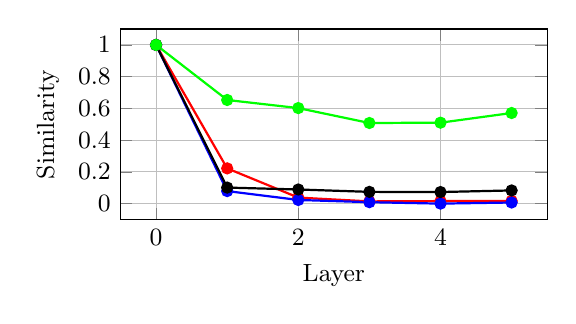
\begin{tikzpicture}
\begin{axis}[
	height=4cm,
	width=7cm,
	xlabel={Layer},
	ylabel={Similarity},
%	xmin=40, xmax=80,
%	ymin=0,  ymax=68,
	legend columns=2,
    legend to name=sanity_leg,
    legend style={font=\footnotesize}
]
	\addplot[mark=*,red] coordinates{(0,1.0)(1,0.222)(2,0.038)(3,0.014)(4,0.016)(5,0.017)};   \leg{Rank Correl (No Abs)}
	\addplot[mark=*,blue] coordinates{(0,1.0)(1,0.079)(2,0.023)(3,0.009)(4,0.000)(5,0.007)}; \leg{Rank Correl (Abs)}
	\addplot[mark=*,black] coordinates{(0,1.0)(1,0.101)(2,0.089)(3,0.074)(4,0.073)(5,0.083)}; \leg{HOGs similarity}
	\addplot[mark=*,green] coordinates{(0,1.0)(1,0.653)(2,0.602)(3,0.508)(4,0.510)(5,0.571)}; \leg{SSIM}
\end{axis}
\end{tikzpicture}
}
\caption{\emph{Sanity check} of Opti-CAM on $1,000$ images of ImageNet validation set using ResNet50. Similarity between saliency maps by original and randomized network, where layers are progressively replaced by random ones.}
\label{fig:sanity}
\end{figure}
%------------------------------------------------------------------------------

%------------------------------------------------------------------------------
\begin{figure}[htpb]
\newcommand{\sizeP}{.12}
\newcommand{\sizeS}{.15}
\newcommand{\hh}{.175\textwidth}
\newcommand{\ww}{.200\textwidth}
\centering
\small
\setlength{\tabcolsep}{3pt}
\begin{tabular}{cccccc}
Original & layer 1 & layer 2 & layer 3 & layer 4 & layer 5 \\
\fig[\sizeS]{sanityC/ILSVRC2012_val_00000001JPEG_0_Smap.png} &
\fig[\sizeS]{sanityC/ILSVRC2012_val_00000001JPEG_1_Smap.png} &
\fig[\sizeS]{sanityC/ILSVRC2012_val_00000001JPEG_2_Smap.png} &
\fig[\sizeS]{sanityC/ILSVRC2012_val_00000001JPEG_3_Smap.png} &
\fig[\sizeS]{sanityC/ILSVRC2012_val_00000001JPEG_4_Smap.png} &
\fig[\sizeS]{sanityC/ILSVRC2012_val_00000001JPEG_6_Smap.png} \\
\fig[\sizeS]{sanityC/ILSVRC2012_val_00000002JPEG_0_Smap.png} &
\fig[\sizeS]{sanityC/ILSVRC2012_val_00000002JPEG_1_Smap.png} &
\fig[\sizeS]{sanityC/ILSVRC2012_val_00000002JPEG_2_Smap.png} &
\fig[\sizeS]{sanityC/ILSVRC2012_val_00000002JPEG_3_Smap.png} &
\fig[\sizeS]{sanityC/ILSVRC2012_val_00000002JPEG_4_Smap.png} &
\fig[\sizeS]{sanityC/ILSVRC2012_val_00000002JPEG_6_Smap.png} \\
\end{tabular}
\caption{\emph{Sanity check visualization} of Opti-CAM on two images of ImageNet validation set using ResNet50. First column: Opti-CAM saliency maps for the original network; remaining columns: Opti-CAM saliency maps where layers are progressively replaced by random ones.}
\label{fig:sanity-vis}
\end{figure}
%------------------------------------------------------------------------------

\section{Sanity check}
\label{sec:sanity-check}

We use the model parameter randomization test proposed by~\citep{adebayosanity}. This test compares the saliency maps generated by a trained model with the ones generated by a partially randomly initialized network of the same architecture. In particular, we choose 5 layers of ResNet50 and we progressively replace them by random ones so that we have 6 different models with different amount of random parameters. The saliency maps are generated for the small subset of ImageNet validation set, as in the ablation study.

Following~\citep{adebayosanity}, we compute a number of similarity metrics between these saliency maps generated by the original and the randomized network, including Rank Correlation with/without absolute values, HOGs similarity, and SSIM. The results are shown in \autoref{fig:sanity} (saliency map similarity measurements) and \autoref{fig:sanity-vis} (saliency map visualizations). Our method passes the sanity check, as it is very sensitive to changes in the model parameters. \modify{We also use model parameter randomization test and train a ResNet50 with randomly permuted labels following the training recipes from the pytorch models\footnote{\url{https://github.com/pytorch/vision/tree/main/references/classification}}. The SSIM similarity is $0.013$, which shows that Opti-CAM is sensitive to the relationship between instances and labels.}

%------------------------------------------------------------------------------
\begin{table}[htbp]
\centering
\footnotesize
\setlength{\tabcolsep}{4pt}
\renewcommand{\arraystretch}{0.8}
\begin{tabular}{lrrrr|rrrr} \toprule
\mr{2}{\Th{Method}}                                & \mc{4}{\Th{ResNet50}} & \mc{4}{\Th{VGG16}} \\ \cmidrule{2-9}
                                                   & {$\AD\!\downarrow$} & {$\AG\!\uparrow$} & {$\AI\!\uparrow$} & \mc{1}{T} & {$\AD\!\downarrow$} & {$\AG\!\uparrow$} & {$\AI\!\uparrow$} & \mc{1}{T} \\ \midrule
Fake-CAM~\citep{poppi2021revisiting}               &0.9&0.7&47.4&0.00&0.5&0.3&47.7&0.00  \\ \midrule
Grad-CAM~\citep{selvaraju2017grad}       & 36.4      &5.5& 27.0      &0.03     & 41.6     &3.3 & 25.2       &0.02     \\
Grad-CAM++~\cite{chattopadhay2018grad}    & 37.6    & 4.9 & 24.0       &0.04    & 46.3     &2.0 & 19.0        &0.02    \\
Score-CAM~\citep{wang2020score}           & 28.8     &8.8 & 33.6       &20.47& 39.3    & 3.5 & 24.6       &3.08     \\
Ablation-CAM~\citep{ramaswamy2020ablation}   & 36.6      &5.1& 25.6      &18.49 & 41.8     & 2.9& 24.0       &2.95    \\
XGrad-CAM~\citep{fu2020axiom}            & 36.4     &5.5 & 27.0       &0.03   & 40.6     &3.4 & 25.8       &0.02   \\
Layer-CAM~\citep{jiang2021layercam} &42.6&4.2&19.2&0.02&82.1&0.3&6.9&0.01   \\
ExPerturbation~\citep{fong2019understanding} &51.2&6.9&26.1&15.67&50.1&4.4&24.5&9.10  \\
\rowcolor{cyan!10}
Opti-CAM (ours)                          &\tb{2.0}&\tb{49.4}&\tb{91.2}&3.94&\tb{1.5}&\tb{52.7}&\tb{92.1}&3.95\\
\bottomrule
\end{tabular}
% \vspace{6pt}
\caption{
\emph{Classification metrics} on ImageNet validation set, without input normalization. AD/AI: average drop/increase~\citep{chattopadhay2018grad}; $\AG$: average gain (ours); $\downarrow$ / $\uparrow$: lower / higher is better. T: Average time (sec) per batch of 8 images. Bold: best, excluding Fake-CAM.}
\label{tab:norm-imagenet}
\end{table}
%------------------------------------------------------------------------------

\section{Results without input normalization}
\label{sec:without-norm}

It is standard that images are normalized to zero mean and unit standard deviation before feeding them to a network, because this is how networks are trained. For example, for ImageNet images, we subtract the mean vector $[0.485,0.456,0.406]$ and divide channel-wise by standard deviation $[0.229,0.224,0.225]$. By doing so however, we cannot reproduce the results published for several baseline methods; rather, all results are improved dramatically. We can obtain results similar to published ones by \emph{not} normalizing, thus we speculate that authors of related work do not normalize images. This is also suggested by our attempts to communicate with the authors.

We believe normalization is important and we include it in all our experiments. For reference and to allow for comparison with published results, we provide results without normalization in \autoref{tab:norm-imagenet} that correspond to \autoref{tab:imagenet-cnn}. Finally, code is provided to allow for the reproduction and verification of our results.

% %------------------------------------------------------------------------------
% % \input{tex/IN_n_chest_n_kvasir_vgg16}
% \begin{figure*}
% \vspace{-0.4cm}
\newcommand{\sizeS}{.12}
\centering
\footnotesize
\setlength{\tabcolsep}{1pt}
\begin{tabular}{c cccc cccc}
     & \mc{4}{VGG16} & \mc{4}{ResNet50}\\
	Input image  &  Grad-CAM  & G-CAM++ & Score-CAM & Opti-CAM  &Grad-CAM  & G-CAM++ & Score-CAM & Opti-CAM \\
	\fig[\sizeS]{medical/chest_Resnet50_GradCAM_0_0img.png} &
	\fig[\sizeS]{medical/chest_VGG16_GradCAM_0_0vis.png} &\fig[\sizeS]{medical/chest_Resnet50_GradCAM_0_0vis.png} &
	\fig[\sizeS]{medical/chest_VGG16_GradCAMPlusPlus_0_0vis.png} &\fig[\sizeS]{medical/chest_Resnet50_GradCAMPlusPlus_0_0vis.png} &
	\fig[\sizeS]{medical/chest_VGG16_ScoreCAM_0_0vis.png} &\fig[\sizeS]{medical/chest_Resnet50_ScoreCAM_0_0vis.png} &
	\fig[\sizeS]{medical/chest_VGG16_OptCAM_0_0vis.png} & \fig[\sizeS]{medical/chest_Resnet50_OptCAM_0_0vis.png} \\
 
\fig[\sizeS]{medical/chest_Resnet50_GradCAM_0_1img.png} &
	\fig[\sizeS]{medical/chest_VGG16_GradCAM_0_1vis.png} &\fig[\sizeS]{medical/chest_Resnet50_GradCAM_0_1vis.png} &
	\fig[\sizeS]{medical/chest_VGG16_GradCAMPlusPlus_0_1vis.png} &\fig[\sizeS]{medical/chest_Resnet50_GradCAMPlusPlus_0_1vis.png} &
	\fig[\sizeS]{medical/chest_VGG16_ScoreCAM_0_1vis.png} &\fig[\sizeS]{medical/chest_Resnet50_ScoreCAM_0_1vis.png} &
	\fig[\sizeS]{medical/chest_VGG16_OptCAM_0_1vis.png} & \fig[\sizeS]{medical/chest_Resnet50_OptCAM_0_1vis.png} \\
 
\fig[\sizeS]{medical/chest_Resnet50_GradCAM_0_2img.png} &
	\fig[\sizeS]{medical/chest_VGG16_GradCAM_0_2vis.png} &\fig[\sizeS]{medical/chest_Resnet50_GradCAM_0_2vis.png} &
	\fig[\sizeS]{medical/chest_VGG16_GradCAMPlusPlus_0_2vis.png} &\fig[\sizeS]{medical/chest_Resnet50_GradCAMPlusPlus_0_2vis.png} &
	\fig[\sizeS]{medical/chest_VGG16_ScoreCAM_0_2vis.png} &\fig[\sizeS]{medical/chest_Resnet50_ScoreCAM_0_2vis.png} &
	\fig[\sizeS]{medical/chest_VGG16_OptCAM_0_2vis.png} & \fig[\sizeS]{medical/chest_Resnet50_OptCAM_0_2vis.png} \\
 
\fig[\sizeS]{medical/chest_Resnet50_GradCAM_0_3img.png} &
	\fig[\sizeS]{medical/chest_VGG16_GradCAM_0_3vis.png} &\fig[\sizeS]{medical/chest_Resnet50_GradCAM_0_3vis.png} &
	\fig[\sizeS]{medical/chest_VGG16_GradCAMPlusPlus_0_3vis.png} &\fig[\sizeS]{medical/chest_Resnet50_GradCAMPlusPlus_0_3vis.png} &
	\fig[\sizeS]{medical/chest_VGG16_ScoreCAM_0_3vis.png} &\fig[\sizeS]{medical/chest_Resnet50_ScoreCAM_0_3vis.png} &
	\fig[\sizeS]{medical/chest_VGG16_OptCAM_0_3vis.png} & \fig[\sizeS]{medical/chest_Resnet50_OptCAM_0_3vis.png} \\
 
	\fig[\sizeS]{medical/chest_Resnet50_GradCAM_1_4img.png} &
	\fig[\sizeS]{medical/chest_VGG16_GradCAM_1_4vis.png} &\fig[\sizeS]{medical/chest_Resnet50_GradCAM_1_4vis.png} &
	\fig[\sizeS]{medical/chest_VGG16_GradCAMPlusPlus_1_4vis.png} &\fig[\sizeS]{medical/chest_Resnet50_GradCAMPlusPlus_1_4vis.png} &
	\fig[\sizeS]{medical/chest_VGG16_ScoreCAM_1_4vis.png} &\fig[\sizeS]{medical/chest_Resnet50_ScoreCAM_1_4vis.png} &
	\fig[\sizeS]{medical/chest_VGG16_OptCAM_1_4vis.png} & \fig[\sizeS]{medical/chest_Resnet50_OptCAM_1_4vis.png} \\

 \fig[\sizeS]{medical/chest_Resnet50_GradCAM_1_5img.png} &
	\fig[\sizeS]{medical/chest_VGG16_GradCAM_1_5vis.png} &\fig[\sizeS]{medical/chest_Resnet50_GradCAM_1_5vis.png} &
	\fig[\sizeS]{medical/chest_VGG16_GradCAMPlusPlus_1_5vis.png} &\fig[\sizeS]{medical/chest_Resnet50_GradCAMPlusPlus_1_5vis.png} &
	\fig[\sizeS]{medical/chest_VGG16_ScoreCAM_1_5vis.png} &\fig[\sizeS]{medical/chest_Resnet50_ScoreCAM_1_5vis.png} &
	\fig[\sizeS]{medical/chest_VGG16_OptCAM_1_5vis.png} & \fig[\sizeS]{medical/chest_Resnet50_OptCAM_1_5vis.png} \\

 \fig[\sizeS]{medical/chest_Resnet50_GradCAM_1_6img.png} &
	\fig[\sizeS]{medical/chest_VGG16_GradCAM_1_6vis.png} &\fig[\sizeS]{medical/chest_Resnet50_GradCAM_1_6vis.png} &
	\fig[\sizeS]{medical/chest_VGG16_GradCAMPlusPlus_1_6vis.png} &\fig[\sizeS]{medical/chest_Resnet50_GradCAMPlusPlus_1_6vis.png} &
	\fig[\sizeS]{medical/chest_VGG16_ScoreCAM_1_6vis.png} &\fig[\sizeS]{medical/chest_Resnet50_ScoreCAM_1_6vis.png} &
	\fig[\sizeS]{medical/chest_VGG16_OptCAM_1_6vis.png} & \fig[\sizeS]{medical/chest_Resnet50_OptCAM_1_6vis.png} \\

 \fig[\sizeS]{medical/chest_Resnet50_GradCAM_1_7img.png} &
	\fig[\sizeS]{medical/chest_VGG16_GradCAM_1_7vis.png} &\fig[\sizeS]{medical/chest_Resnet50_GradCAM_1_7vis.png} &
	\fig[\sizeS]{medical/chest_VGG16_GradCAMPlusPlus_1_7vis.png} &\fig[\sizeS]{medical/chest_Resnet50_GradCAMPlusPlus_1_7vis.png} &
	\fig[\sizeS]{medical/chest_VGG16_ScoreCAM_1_7vis.png} &\fig[\sizeS]{medical/chest_Resnet50_ScoreCAM_1_7vis.png} &
	\fig[\sizeS]{medical/chest_VGG16_OptCAM_1_7vis.png} & \fig[\sizeS]{medical/chest_Resnet50_OptCAM_1_7vis.png} \\
\end{tabular}
\caption{Saliency maps obtained from Chest X-ray images.}
\label{fig:vis-chest-resnet}
% \vspace{-0.8cm}
\end{figure*}

% 
\begin{figure*}
\newcommand{\sizeS}{.12}
\centering
\footnotesize
\setlength{\tabcolsep}{1pt}
\begin{tabular}{c cccc cccc}
     & \mc{4}{VGG16} & \mc{4}{ResNet50}\\
	Input image  &  Grad-CAM  & G-CAM++ & Score-CAM & Opti-CAM  &Grad-CAM  & G-CAM++ & Score-CAM & Opti-CAM \\
	\fig[\sizeS]{medical/kvasir_Resnet50_GradCAM_0_img.png} &
	\fig[\sizeS]{medical/kvasir_VGG16_GradCAM_0_vis.png} &
	\fig[\sizeS]{medical/kvasir_VGG16_GradCAMPlusPlus_0_vis.png} &
	\fig[\sizeS]{medical/kvasir_VGG16_ScoreCAM_0_vis.png} &
	\fig[\sizeS]{medical/kvasir_VGG16_OptCAM_0_vis.png} &
		\fig[\sizeS]{medical/kvasir_Resnet50_GradCAM_0_vis.png} &
	\fig[\sizeS]{medical/kvasir_Resnet50_GradCAMPlusPlus_0_vis.png} &
	\fig[\sizeS]{medical/kvasir_Resnet50_ScoreCAM_0_vis.png} &
	\fig[\sizeS]{medical/kvasir_Resnet50_OptCAM_0_vis.png}
	\\
	\fig[\sizeS]{medical/kvasir_VGG16_GradCAM_1_img.png} &
	\fig[\sizeS]{medical/kvasir_VGG16_GradCAM_1_vis.png} &
	\fig[\sizeS]{medical/kvasir_VGG16_GradCAMPlusPlus_1_vis.png} &
	\fig[\sizeS]{medical/kvasir_VGG16_ScoreCAM_1_vis.png} &
	\fig[\sizeS]{medical/kvasir_VGG16_OptCAM_1_vis.png} &
	\fig[\sizeS]{medical/kvasir_Resnet50_GradCAM_1_vis.png} &
	\fig[\sizeS]{medical/kvasir_Resnet50_GradCAMPlusPlus_1_vis.png} &
	\fig[\sizeS]{medical/kvasir_Resnet50_ScoreCAM_1_vis.png} &
	\fig[\sizeS]{medical/kvasir_Resnet50_OptCAM_1_vis.png} 
	
	\\
	\fig[\sizeS]{medical/kvasir_VGG16_GradCAM_2_img.png} &
	\fig[\sizeS]{medical/kvasir_VGG16_GradCAM_2_vis.png} &
	\fig[\sizeS]{medical/kvasir_VGG16_GradCAMPlusPlus_2_vis.png} &
	\fig[\sizeS]{medical/kvasir_VGG16_ScoreCAM_2_vis.png} &
	\fig[\sizeS]{medical/kvasir_VGG16_OptCAM_2_vis.png} &
	\fig[\sizeS]{medical/kvasir_Resnet50_GradCAM_2_vis.png} &
	\fig[\sizeS]{medical/kvasir_Resnet50_GradCAMPlusPlus_2_vis.png} &
	\fig[\sizeS]{medical/kvasir_Resnet50_ScoreCAM_2_vis.png} &
	\fig[\sizeS]{medical/kvasir_Resnet50_OptCAM_2_vis.png}\\
	
	
	\fig[\sizeS]{medical/kvasir_Resnet50_GradCAM_3_img.png} &
	\fig[\sizeS]{medical/kvasir_VGG16_GradCAM_3_vis.png} &
	\fig[\sizeS]{medical/kvasir_VGG16_GradCAMPlusPlus_3_vis.png} &
	\fig[\sizeS]{medical/kvasir_VGG16_ScoreCAM_3_vis.png} &
	\fig[\sizeS]{medical/kvasir_VGG16_OptCAM_3_vis.png} &
	\fig[\sizeS]{medical/kvasir_Resnet50_GradCAM_3_vis.png} &
	\fig[\sizeS]{medical/kvasir_Resnet50_GradCAMPlusPlus_3_vis.png} &
	\fig[\sizeS]{medical/kvasir_Resnet50_ScoreCAM_3_vis.png} &
	\fig[\sizeS]{medical/kvasir_Resnet50_OptCAM_3_vis.png}
	\\
	\fig[\sizeS]{medical/kvasir_Resnet50_GradCAM_4_img.png} &
	\fig[\sizeS]{medical/kvasir_VGG16_GradCAM_4_vis.png} &
	\fig[\sizeS]{medical/kvasir_VGG16_GradCAMPlusPlus_4_vis.png} &
	\fig[\sizeS]{medical/kvasir_VGG16_ScoreCAM_4_vis.png} &
	\fig[\sizeS]{medical/kvasir_VGG16_OptCAM_4_vis.png} &
	\fig[\sizeS]{medical/kvasir_Resnet50_GradCAM_4_vis.png} &
	\fig[\sizeS]{medical/kvasir_Resnet50_GradCAMPlusPlus_4_vis.png} &
	\fig[\sizeS]{medical/kvasir_Resnet50_ScoreCAM_4_vis.png} &
	\fig[\sizeS]{medical/kvasir_Resnet50_OptCAM_4_vis.png}
	\\
	\fig[\sizeS]{medical/kvasir_Resnet50_GradCAM_5_img.png} &
	\fig[\sizeS]{medical/kvasir_VGG16_GradCAM_5_vis.png} &
	\fig[\sizeS]{medical/kvasir_VGG16_GradCAMPlusPlus_5_vis.png} &
	\fig[\sizeS]{medical/kvasir_VGG16_ScoreCAM_5_vis.png} &
	\fig[\sizeS]{medical/kvasir_VGG16_OptCAM_5_vis.png}  &
	\fig[\sizeS]{medical/kvasir_Resnet50_GradCAM_5_vis.png} &
	\fig[\sizeS]{medical/kvasir_Resnet50_GradCAMPlusPlus_5_vis.png} &
	\fig[\sizeS]{medical/kvasir_Resnet50_ScoreCAM_5_vis.png} &
	\fig[\sizeS]{medical/kvasir_Resnet50_OptCAM_5_vis.png} 
	\\
	\fig[\sizeS]{medical/kvasir_Resnet50_GradCAM_6_img.png} &
	\fig[\sizeS]{medical/kvasir_VGG16_GradCAM_6_vis.png} &
	\fig[\sizeS]{medical/kvasir_VGG16_GradCAMPlusPlus_6_vis.png} &
	\fig[\sizeS]{medical/kvasir_VGG16_ScoreCAM_6_vis.png} &
	\fig[\sizeS]{medical/kvasir_VGG16_OptCAM_6_vis.png} &
	\fig[\sizeS]{medical/kvasir_Resnet50_GradCAM_6_vis.png} &
	\fig[\sizeS]{medical/kvasir_Resnet50_GradCAMPlusPlus_6_vis.png} &
	\fig[\sizeS]{medical/kvasir_Resnet50_ScoreCAM_6_vis.png} &
	\fig[\sizeS]{medical/kvasir_Resnet50_OptCAM_6_vis.png} 
	\\
	\fig[\sizeS]{medical/kvasir_Resnet50_GradCAM_7_img.png} &
	\fig[\sizeS]{medical/kvasir_VGG16_GradCAM_7_vis.png} &
	\fig[\sizeS]{medical/kvasir_VGG16_GradCAMPlusPlus_7_vis.png} &
	\fig[\sizeS]{medical/kvasir_VGG16_ScoreCAM_7_vis.png} &
	\fig[\sizeS]{medical/kvasir_VGG16_OptCAM_7_vis.png} &
	\fig[\sizeS]{medical/kvasir_Resnet50_GradCAM_7_vis.png} &
	\fig[\sizeS]{medical/kvasir_Resnet50_GradCAMPlusPlus_7_vis.png} &
	\fig[\sizeS]{medical/kvasir_Resnet50_ScoreCAM_7_vis.png} &
	\fig[\sizeS]{medical/kvasir_Resnet50_OptCAM_7_vis.png} \\
\end{tabular}
\caption{Saliency maps obtained for KVASIR images.}
\label{fig:vis-kvasir-resnet}
\end{figure*}



% \begin{figure*}[t]
\newcommand{\sizeP}{.14}
\newcommand{\sizeS}{.14}
\newcommand{\hh}{.175\textwidth}
\newcommand{\ww}{.200\textwidth}
\scriptsize
\centering
\setlength{\tabcolsep}{3pt}
\begin{tabular}{ccccccc}
	Input image  &  Grad-CAM  & G-CAM++ & Score-CAM & Ablation-CAM & XG-CAM & Opti-CAM (ours) \\
        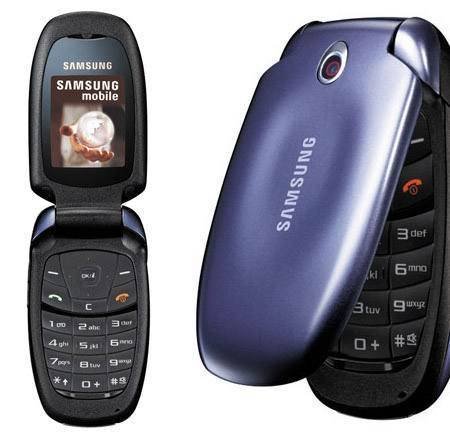
\includegraphics[trim={12mm 14mm 12mm 14mm},clip, width=\sizeP\textwidth]{fig/visual/ILSVRC2012_val_00000089.JPEG}&
	\fig[\sizeS]{visual/VGG16_GradCAM_ILSVRC2012_val_00000089.png} &
	\fig[\sizeS]{visual/VGG16_GradCAMPlusPlus_ILSVRC2012_val_00000089.png} &
	\fig[\sizeS]{visual/VGG16_ScoreCAM_ILSVRC2012_val_00000089.png} &
	\fig[\sizeS]{visual/VGG16_AblationCAM_ILSVRC2012_val_00000089.png} &
	\fig[\sizeS]{visual/VGG16_XGradCAM_ILSVRC2012_val_00000089.png} & 
	\fig[\sizeS]{visual/VGG16_OptCAM_ILSVRC2012_val_00000089.png}  \\
	Cellphone &&&&&& \\
	\fig[\sizeS]{visual/ILSVRC2012_val_00000748.png}&
	\fig[\sizeS]{visual/VGG16_GradCAM_ILSVRC2012_val_00000748.png} &
	\fig[\sizeS]{visual/VGG16_GradCAMPlusPlus_ILSVRC2012_val_00000748.png} &
	\fig[\sizeS]{visual/VGG16_ScoreCAM_ILSVRC2012_val_00000748.png} &
	\fig[\sizeS]{visual/VGG16_AblationCAM_ILSVRC2012_val_00000748.png} &
	\fig[\sizeS]{visual/VGG16_XGradCAM_ILSVRC2012_val_00000748.png} & 
	\fig[\sizeS]{visual/VGG16_OptCAM_ILSVRC2012_val_00000748.png}  \\
	Miniature Schnauzer &&&&&& \\
	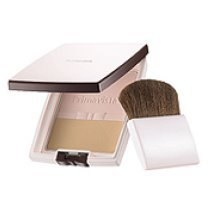
\includegraphics[trim={2mm 3mm 6mm 1mm},clip, width=\sizeP\textwidth]{fig/visual/ILSVRC2012_val_00000769.JPEG}&
	\fig[\sizeS]{visual/VGG16_GradCAM_ILSVRC2012_val_00000769.png} &
	\fig[\sizeS]{visual/VGG16_GradCAMPlusPlus_ILSVRC2012_val_00000769.png} &
	\fig[\sizeS]{visual/VGG16_ScoreCAM_ILSVRC2012_val_00000769.png} &
	\fig[\sizeS]{visual/VGG16_AblationCAM_ILSVRC2012_val_00000769.png} &
	\fig[\sizeS]{visual/VGG16_XGradCAM_ILSVRC2012_val_00000769.png} & 
	\fig[\sizeS]{visual/VGG16_OptCAM_ILSVRC2012_val_00000769.png}  \\
	Face Powder &&&&&& \\
	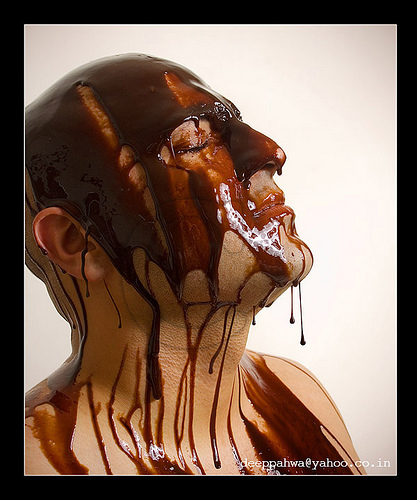
\includegraphics[trim={2mm 6mm 2mm 6mm},clip, width=\sizeP\textwidth]{fig/visual/ILSVRC2012_val_00000782.JPEG}&
	\fig[\sizeS]{visual/VGG16_GradCAM_ILSVRC2012_val_00000782.png} &
	\fig[\sizeS]{visual/VGG16_GradCAMPlusPlus_ILSVRC2012_val_00000782.png} &
	\fig[\sizeS]{visual/VGG16_ScoreCAM_ILSVRC2012_val_00000782.png} &
	\fig[\sizeS]{visual/VGG16_AblationCAM_ILSVRC2012_val_00000782.png} &
	\fig[\sizeS]{visual/VGG16_XGradCAM_ILSVRC2012_val_00000782.png} & 
	\fig[\sizeS]{visual/VGG16_OptCAM_ILSVRC2012_val_00000782.png}  \\
	Chocolate Sauce &&&&&& \\
	\fig[\sizeS]{visual/ILSVRC2012_val_00001113.png}&
	\fig[\sizeS]{visual/VGG16_GradCAM_ILSVRC2012_val_00001113.png} &
	\fig[\sizeS]{visual/VGG16_GradCAMPlusPlus_ILSVRC2012_val_00001113.png} &
	\fig[\sizeS]{visual/VGG16_ScoreCAM_ILSVRC2012_val_00001113.png} &
	\fig[\sizeS]{visual/VGG16_AblationCAM_ILSVRC2012_val_00001113.png} &
	\fig[\sizeS]{visual/VGG16_XGradCAM_ILSVRC2012_val_00001113.png} & 
	\fig[\sizeS]{visual/VGG16_OptCAM_ILSVRC2012_val_00001113.png}  \\
	Komondor &&&&&& \\
 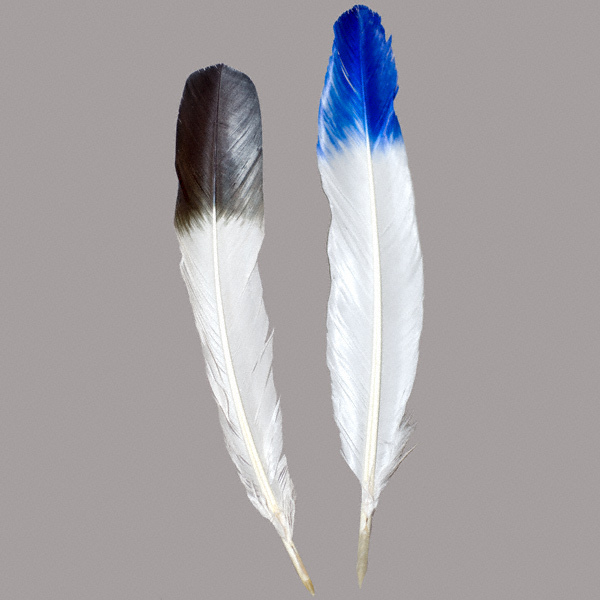
\includegraphics[trim={14mm 16mm 14mm 12mm},clip, width=\sizeP\textwidth]{fig/visual/ILSVRC2012_val_00001345.JPEG}&
	\fig[\sizeS]{visual/VGG16_GradCAM_ILSVRC2012_val_00001345.png} &
	\fig[\sizeS]{visual/VGG16_GradCAMPlusPlus_ILSVRC2012_val_00001345.png} &
	\fig[\sizeS]{visual/VGG16_ScoreCAM_ILSVRC2012_val_00001345.png} &
	\fig[\sizeS]{visual/VGG16_AblationCAM_ILSVRC2012_val_00001345.png} &
	\fig[\sizeS]{visual/VGG16_XGradCAM_ILSVRC2012_val_00001345.png} & 
	\fig[\sizeS]{visual/VGG16_OptCAM_ILSVRC2012_val_00001345.png}  \\
	Quill &&&&&& \\
 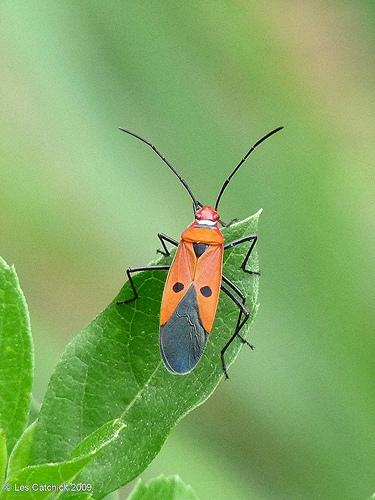
\includegraphics[trim={5mm 14mm 5mm 14mm},clip, width=\sizeP\textwidth]{fig/visual/ILSVRC2012_val_00001529.JPEG}&
	\fig[\sizeS]{visual/VGG16_GradCAM_ILSVRC2012_val_00001529.png} &
	\fig[\sizeS]{visual/VGG16_GradCAMPlusPlus_ILSVRC2012_val_00001529.png} &
	\fig[\sizeS]{visual/VGG16_ScoreCAM_ILSVRC2012_val_00001529.png} &
	\fig[\sizeS]{visual/VGG16_AblationCAM_ILSVRC2012_val_00001529.png} &
	\fig[\sizeS]{visual/VGG16_XGradCAM_ILSVRC2012_val_00001529.png} & 
	\fig[\sizeS]{visual/VGG16_OptCAM_ILSVRC2012_val_00001529.png}  \\
	Longicorn &&&&&& \\
 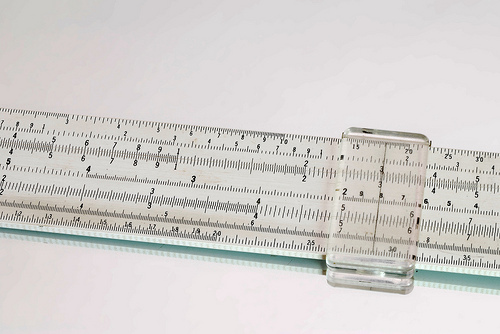
\includegraphics[trim={8mm 1mm 8mm 1mm},clip, width=\sizeP\textwidth]{fig/visual/ILSVRC2012_val_00001635.JPEG}&
	\fig[\sizeS]{visual/VGG16_GradCAM_ILSVRC2012_val_00001635.png} &
	\fig[\sizeS]{visual/VGG16_GradCAMPlusPlus_ILSVRC2012_val_00001635.png} &
	\fig[\sizeS]{visual/VGG16_ScoreCAM_ILSVRC2012_val_00001635.png} &
	\fig[\sizeS]{visual/VGG16_AblationCAM_ILSVRC2012_val_00001635.png} &
	\fig[\sizeS]{visual/VGG16_XGradCAM_ILSVRC2012_val_00001635.png} & 
	\fig[\sizeS]{visual/VGG16_OptCAM_ILSVRC2012_val_00001635.png}  \\
	Slide Rule &&&&&& \\
\end{tabular}
% \vspace{5pt}
\caption{Saliency maps obtained from ImageNet example images using different methods on VGG16.}
\label{fig:imagenet-vis-more-vgg}
\end{figure*}

% \begin{figure*}[t]
\newcommand{\sizeP}{.14}
\newcommand{\sizeS}{.14}
\newcommand{\hh}{.175\textwidth}
\newcommand{\ww}{.200\textwidth}
\scriptsize
\centering
\setlength{\tabcolsep}{3pt}
\begin{tabular}{ccccccc}
	Input image  &  Grad-CAM  & G-CAM++ & Score-CAM & Ablation-CAM & XG-CAM & Opti-CAM (ours) \\
        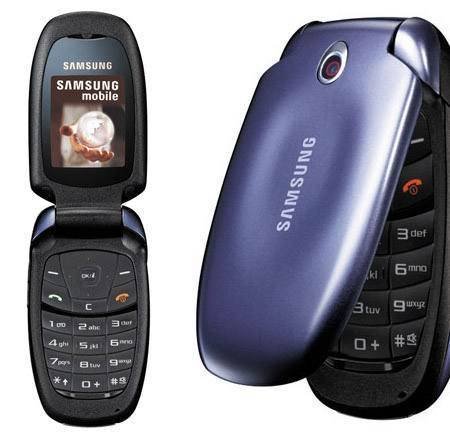
\includegraphics[trim={12mm 14mm 12mm 14mm},clip, width=\sizeP\textwidth]{fig/visual/ILSVRC2012_val_00000089.JPEG}&
	\fig[\sizeS]{visual/Resnet50_GradCAM_ILSVRC2012_val_00000089.png} &
	\fig[\sizeS]{visual/Resnet50_GradCAMPlusPlus_ILSVRC2012_val_00000089.png} &
	\fig[\sizeS]{visual/Resnet50_ScoreCAM_ILSVRC2012_val_00000089.png} &
	\fig[\sizeS]{visual/Resnet50_AblationCAM_ILSVRC2012_val_00000089.png} &
	\fig[\sizeS]{visual/Resnet50_XGradCAM_ILSVRC2012_val_00000089.png} & 
	\fig[\sizeS]{visual/Resnet50_OptCAM_ILSVRC2012_val_00000089.png}  \\
	Cellphone &&&&&& \\
	\fig[\sizeS]{visual/ILSVRC2012_val_00000748.png}&
	\fig[\sizeS]{visual/Resnet50_GradCAM_ILSVRC2012_val_00000748.png} &
	\fig[\sizeS]{visual/Resnet50_GradCAMPlusPlus_ILSVRC2012_val_00000748.png} &
	\fig[\sizeS]{visual/Resnet50_ScoreCAM_ILSVRC2012_val_00000748.png} &
	\fig[\sizeS]{visual/Resnet50_AblationCAM_ILSVRC2012_val_00000748.png} &
	\fig[\sizeS]{visual/Resnet50_XGradCAM_ILSVRC2012_val_00000748.png} & 
	\fig[\sizeS]{visual/Resnet50_OptCAM_ILSVRC2012_val_00000748.png}  \\
	Miniature Schnauzer &&&&&& \\
	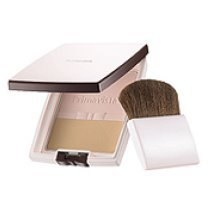
\includegraphics[trim={2mm 3mm 6mm 1mm},clip, width=\sizeP\textwidth]{fig/visual/ILSVRC2012_val_00000769.JPEG}&
	\fig[\sizeS]{visual/Resnet50_GradCAM_ILSVRC2012_val_00000769.png} &
	\fig[\sizeS]{visual/Resnet50_GradCAMPlusPlus_ILSVRC2012_val_00000769.png} &
	\fig[\sizeS]{visual/Resnet50_ScoreCAM_ILSVRC2012_val_00000769.png} &
	\fig[\sizeS]{visual/Resnet50_AblationCAM_ILSVRC2012_val_00000769.png} &
	\fig[\sizeS]{visual/Resnet50_XGradCAM_ILSVRC2012_val_00000769.png} & 
	\fig[\sizeS]{visual/Resnet50_OptCAM_ILSVRC2012_val_00000769.png}  \\
	Face Powder &&&&&& \\
	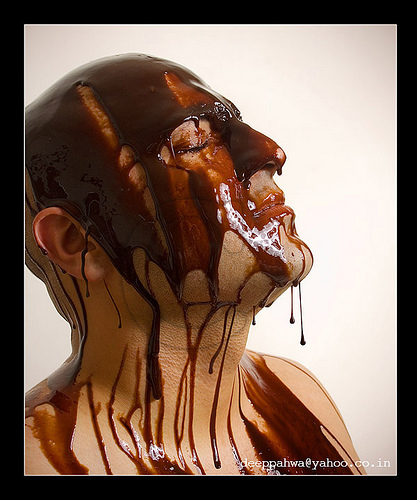
\includegraphics[trim={2mm 6mm 2mm 6mm},clip, width=\sizeP\textwidth]{fig/visual/ILSVRC2012_val_00000782.JPEG}&
	\fig[\sizeS]{visual/Resnet50_GradCAM_ILSVRC2012_val_00000782.png} &
	\fig[\sizeS]{visual/Resnet50_GradCAMPlusPlus_ILSVRC2012_val_00000782.png} &
	\fig[\sizeS]{visual/Resnet50_ScoreCAM_ILSVRC2012_val_00000782.png} &
	\fig[\sizeS]{visual/Resnet50_AblationCAM_ILSVRC2012_val_00000782.png} &
	\fig[\sizeS]{visual/Resnet50_XGradCAM_ILSVRC2012_val_00000782.png} & 
	\fig[\sizeS]{visual/Resnet50_OptCAM_ILSVRC2012_val_00000782.png}  \\
	Chocolate Sauce &&&&&& \\
	\fig[\sizeS]{visual/ILSVRC2012_val_00001113.png}&
	\fig[\sizeS]{visual/Resnet50_GradCAM_ILSVRC2012_val_00001113.png} &
	\fig[\sizeS]{visual/Resnet50_GradCAMPlusPlus_ILSVRC2012_val_00001113.png} &
	\fig[\sizeS]{visual/Resnet50_ScoreCAM_ILSVRC2012_val_00001113.png} &
	\fig[\sizeS]{visual/Resnet50_AblationCAM_ILSVRC2012_val_00001113.png} &
	\fig[\sizeS]{visual/Resnet50_XGradCAM_ILSVRC2012_val_00001113.png} & 
	\fig[\sizeS]{visual/Resnet50_OptCAM_ILSVRC2012_val_00001113.png}  \\
	Komondor &&&&&& \\
 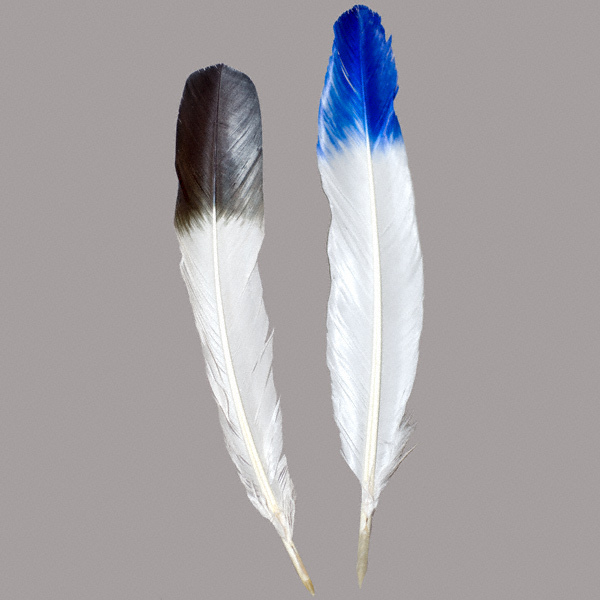
\includegraphics[trim={14mm 16mm 14mm 12mm},clip, width=\sizeP\textwidth]{fig/visual/ILSVRC2012_val_00001345.JPEG}&
	\fig[\sizeS]{visual/Resnet50_GradCAM_ILSVRC2012_val_00001345.png} &
	\fig[\sizeS]{visual/Resnet50_GradCAMPlusPlus_ILSVRC2012_val_00001345.png} &
	\fig[\sizeS]{visual/Resnet50_ScoreCAM_ILSVRC2012_val_00001345.png} &
	\fig[\sizeS]{visual/Resnet50_AblationCAM_ILSVRC2012_val_00001345.png} &
	\fig[\sizeS]{visual/Resnet50_XGradCAM_ILSVRC2012_val_00001345.png} & 
	\fig[\sizeS]{visual/Resnet50_OptCAM_ILSVRC2012_val_00001345.png}  \\
	Quill &&&&&& \\
 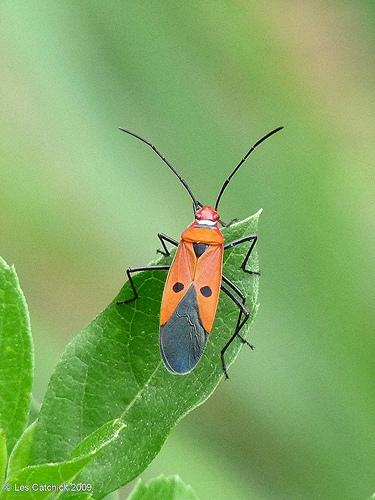
\includegraphics[trim={5mm 14mm 5mm 14mm},clip, width=\sizeP\textwidth]{fig/visual/ILSVRC2012_val_00001529.JPEG}&
	\fig[\sizeS]{visual/Resnet50_GradCAM_ILSVRC2012_val_00001529.png} &
	\fig[\sizeS]{visual/Resnet50_GradCAMPlusPlus_ILSVRC2012_val_00001529.png} &
	\fig[\sizeS]{visual/Resnet50_ScoreCAM_ILSVRC2012_val_00001529.png} &
	\fig[\sizeS]{visual/Resnet50_AblationCAM_ILSVRC2012_val_00001529.png} &
	\fig[\sizeS]{visual/Resnet50_XGradCAM_ILSVRC2012_val_00001529.png} & 
	\fig[\sizeS]{visual/Resnet50_OptCAM_ILSVRC2012_val_00001529.png}  \\
	Longicorn &&&&&& \\
 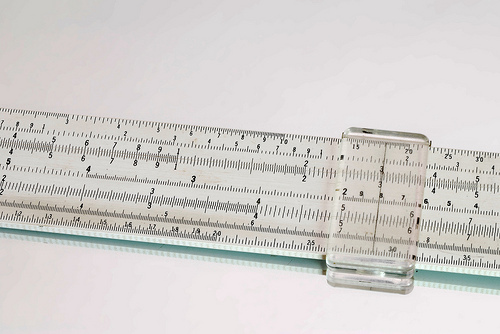
\includegraphics[trim={8mm 1mm 8mm 1mm},clip, width=\sizeP\textwidth]{fig/visual/ILSVRC2012_val_00001635.JPEG}&
	\fig[\sizeS]{visual/Resnet50_GradCAM_ILSVRC2012_val_00001635.png} &
	\fig[\sizeS]{visual/Resnet50_GradCAMPlusPlus_ILSVRC2012_val_00001635.png} &
	\fig[\sizeS]{visual/Resnet50_ScoreCAM_ILSVRC2012_val_00001635.png} &
	\fig[\sizeS]{visual/Resnet50_AblationCAM_ILSVRC2012_val_00001635.png} &
	\fig[\sizeS]{visual/Resnet50_XGradCAM_ILSVRC2012_val_00001635.png} & 
	\fig[\sizeS]{visual/Resnet50_OptCAM_ILSVRC2012_val_00001635.png}  \\
	Slide Rule &&&&&& \\
\end{tabular}
% \vspace{5pt}
\caption{Saliency maps obtained from ImageNet example images using different methods on ResNet50.}
\label{fig:imagenet-vis-more-res}
\end{figure*}

% % \begin{figure*}[t]
\newcommand{\sizeP}{.12}
\newcommand{\sizeS}{.12}
\newcommand{\hh}{.175\textwidth}
\newcommand{\ww}{.200\textwidth}
\tiny
\centering
\setlength{\tabcolsep}{1pt}
\begin{tabular}{cccccccc}
	Input image  &  Grad-CAM  & G-CAM++ & Score-CAM & XG-CAM & Raw Att. & Rollout & Opti-CAM (ours) \\
        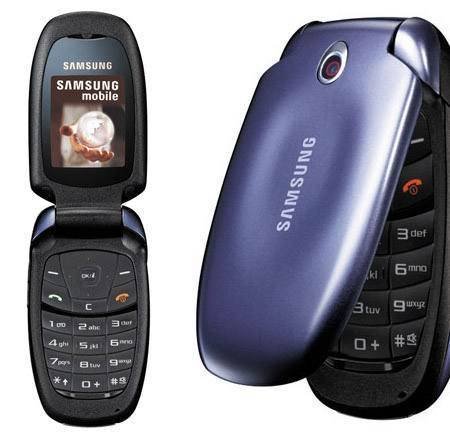
\includegraphics[trim={12mm 14mm 12mm 14mm},clip, width=\sizeP\textwidth]{fig/visual/ILSVRC2012_val_00000089.JPEG}&
	\fig[\sizeS]{visual/ViT_GradCAM_ILSVRC2012_val_00000089.png} &
	\fig[\sizeS]{visual/ViT_GradCAMPlusPlus_ILSVRC2012_val_00000089.png} &
	\fig[\sizeS]{visual/ViT_ScoreCAM_ILSVRC2012_val_00000089.png} &
	\fig[\sizeS]{visual/ViT_XGradCAM_ILSVRC2012_val_00000089.png} & 
        \fig[\sizeS]{visual/ViT_RawAttention_ILSVRC2012_val_00000089.png} &
        \fig[\sizeS]{visual/ViT_RolloutMean_ILSVRC2012_val_00000089.png} &
	\fig[\sizeS]{visual/ViT_OptiCAM_ILSVRC2012_val_00000089.png}  \\
	Cellphone &&&&&& \\
	\fig[\sizeS]{visual/ILSVRC2012_val_00000748.png}&
	\fig[\sizeS]{visual/ViT_GradCAM_ILSVRC2012_val_00000748.png} &
	\fig[\sizeS]{visual/ViT_GradCAMPlusPlus_ILSVRC2012_val_00000748.png} &
	\fig[\sizeS]{visual/ViT_ScoreCAM_ILSVRC2012_val_00000748.png} &
	\fig[\sizeS]{visual/ViT_XGradCAM_ILSVRC2012_val_00000748.png} & 
        \fig[\sizeS]{visual/ViT_RawAttention_ILSVRC2012_val_00000748.png} &
        \fig[\sizeS]{visual/ViT_RolloutMean_ILSVRC2012_val_00000748.png} &
	\fig[\sizeS]{visual/ViT_OptiCAM_ILSVRC2012_val_00000748.png}  \\
	Miniature Schnauzer &&&&&& \\
	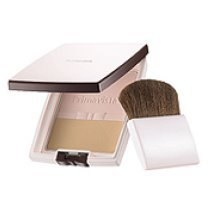
\includegraphics[trim={2mm 3mm 6mm 1mm},clip, width=\sizeP\textwidth]{fig/visual/ILSVRC2012_val_00000769.JPEG}&
	\fig[\sizeS]{visual/ViT_GradCAM_ILSVRC2012_val_00000769.png} &
	\fig[\sizeS]{visual/ViT_GradCAMPlusPlus_ILSVRC2012_val_00000769.png} &
	\fig[\sizeS]{visual/ViT_ScoreCAM_ILSVRC2012_val_00000769.png} &
	\fig[\sizeS]{visual/ViT_XGradCAM_ILSVRC2012_val_00000769.png} & 
        \fig[\sizeS]{visual/ViT_RawAttention_ILSVRC2012_val_00000769.png} &
        \fig[\sizeS]{visual/ViT_RolloutMean_ILSVRC2012_val_00000769.png} &
	\fig[\sizeS]{visual/ViT_OptiCAM_ILSVRC2012_val_00000769.png}  \\
	Face Powder &&&&&& \\
	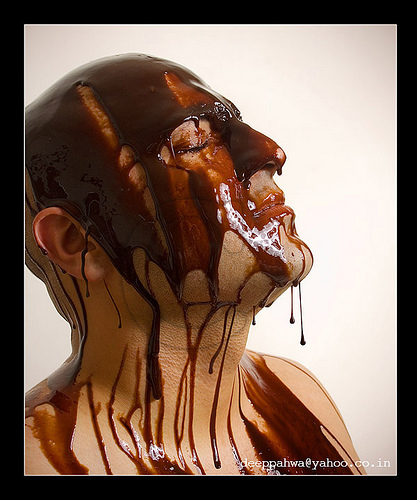
\includegraphics[trim={2mm 6mm 2mm 6mm},clip, width=\sizeP\textwidth]{fig/visual/ILSVRC2012_val_00000782.JPEG}&
	\fig[\sizeS]{visual/ViT_GradCAM_ILSVRC2012_val_00000782.png} &
	\fig[\sizeS]{visual/ViT_GradCAMPlusPlus_ILSVRC2012_val_00000782.png} &
	\fig[\sizeS]{visual/ViT_ScoreCAM_ILSVRC2012_val_00000782.png} &
	\fig[\sizeS]{visual/ViT_XGradCAM_ILSVRC2012_val_00000782.png} & 
        \fig[\sizeS]{visual/ViT_RawAttention_ILSVRC2012_val_00000782.png} &
        \fig[\sizeS]{visual/ViT_RolloutMean_ILSVRC2012_val_00000782.png} &
	\fig[\sizeS]{visual/ViT_OptiCAM_ILSVRC2012_val_00000782.png}  \\
	Chocolate Sauce &&&&&& \\
	\fig[\sizeS]{visual/ILSVRC2012_val_00001113.png}&
	\fig[\sizeS]{visual/ViT_GradCAM_ILSVRC2012_val_00001113.png} &
	\fig[\sizeS]{visual/ViT_GradCAMPlusPlus_ILSVRC2012_val_00001113.png} &
	\fig[\sizeS]{visual/ViT_ScoreCAM_ILSVRC2012_val_00001113.png} &
	\fig[\sizeS]{visual/ViT_XGradCAM_ILSVRC2012_val_00001113.png} & 
        \fig[\sizeS]{visual/ViT_RawAttention_ILSVRC2012_val_00001113.png} &
        \fig[\sizeS]{visual/ViT_RolloutMean_ILSVRC2012_val_00001113.png} &
	\fig[\sizeS]{visual/ViT_OptiCAM_ILSVRC2012_val_00001113.png}  \\
	Komondor &&&&&& \\
 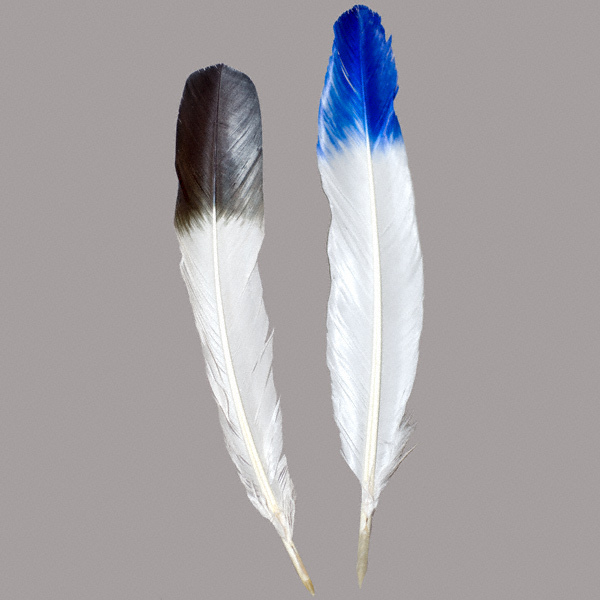
\includegraphics[trim={14mm 16mm 14mm 12mm},clip, width=\sizeP\textwidth]{fig/visual/ILSVRC2012_val_00001345.JPEG}&
	\fig[\sizeS]{visual/ViT_GradCAM_ILSVRC2012_val_00001345.png} &
	\fig[\sizeS]{visual/ViT_GradCAMPlusPlus_ILSVRC2012_val_00001345.png} &
	\fig[\sizeS]{visual/ViT_ScoreCAM_ILSVRC2012_val_00001345.png} &
	\fig[\sizeS]{visual/ViT_XGradCAM_ILSVRC2012_val_00001345.png} & 
        \fig[\sizeS]{visual/ViT_RawAttention_ILSVRC2012_val_00001345.png} &
        \fig[\sizeS]{visual/ViT_RolloutMean_ILSVRC2012_val_00001345.png} &
	\fig[\sizeS]{visual/ViT_OptiCAM_ILSVRC2012_val_00001345.png}  \\
	Quill &&&&&& \\
 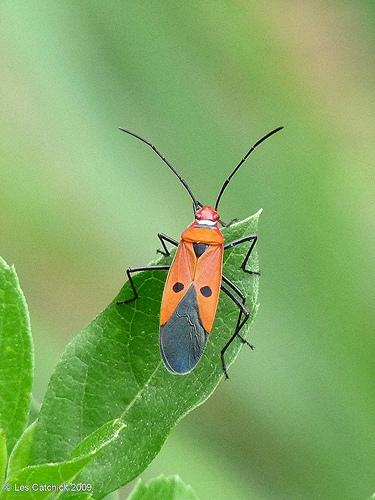
\includegraphics[trim={5mm 14mm 5mm 14mm},clip, width=\sizeP\textwidth]{fig/visual/ILSVRC2012_val_00001529.JPEG}&
	\fig[\sizeS]{visual/ViT_GradCAM_ILSVRC2012_val_00001529.png} &
	\fig[\sizeS]{visual/ViT_GradCAMPlusPlus_ILSVRC2012_val_00001529.png} &
	\fig[\sizeS]{visual/ViT_ScoreCAM_ILSVRC2012_val_00001529.png} &
	\fig[\sizeS]{visual/ViT_XGradCAM_ILSVRC2012_val_00001529.png} & 
        \fig[\sizeS]{visual/ViT_RawAttention_ILSVRC2012_val_00001529.png} &
        \fig[\sizeS]{visual/ViT_RolloutMean_ILSVRC2012_val_00001529.png} &
	\fig[\sizeS]{visual/ViT_OptiCAM_ILSVRC2012_val_00001529.png}  \\
	Longicorn &&&&&& \\
 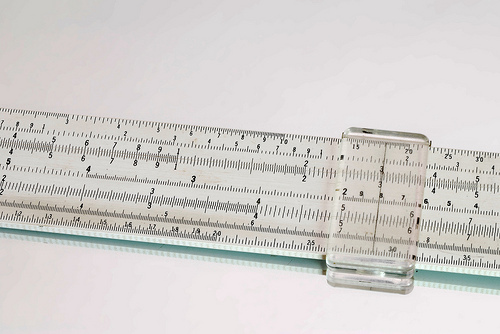
\includegraphics[trim={8mm 1mm 8mm 1mm},clip, width=\sizeP\textwidth]{fig/visual/ILSVRC2012_val_00001635.JPEG}&
	\fig[\sizeS]{visual/ViT_GradCAM_ILSVRC2012_val_00001635.png} &
	\fig[\sizeS]{visual/ViT_GradCAMPlusPlus_ILSVRC2012_val_00001635.png} &
	\fig[\sizeS]{visual/ViT_ScoreCAM_ILSVRC2012_val_00001635.png} &
	\fig[\sizeS]{visual/ViT_XGradCAM_ILSVRC2012_val_00001635.png} & 
        \fig[\sizeS]{visual/ViT_RawAttention_ILSVRC2012_val_00001635.png} &
        \fig[\sizeS]{visual/ViT_RolloutMean_ILSVRC2012_val_00001635.png} &
	\fig[\sizeS]{visual/ViT_OptiCAM_ILSVRC2012_val_00001635.png}  \\
	Slide Rule &&&&&& \\
\end{tabular}
% \vspace{5pt}
\caption{Saliency maps obtained from ImageNet example images using different methods on ViT.}
\label{fig:imagenet-vis-more-vit}
\end{figure*}

% % \begin{figure*}[t]
\newcommand{\sizeP}{.12}
\newcommand{\sizeS}{.12}
\newcommand{\hh}{.175\textwidth}
\newcommand{\ww}{.200\textwidth}
\tiny
\centering
\setlength{\tabcolsep}{1pt}
\begin{tabular}{cccccccc}
	Input image  &  Grad-CAM  & G-CAM++ & Score-CAM & XG-CAM & Raw Att. & Rollout & Opti-CAM (ours) \\
        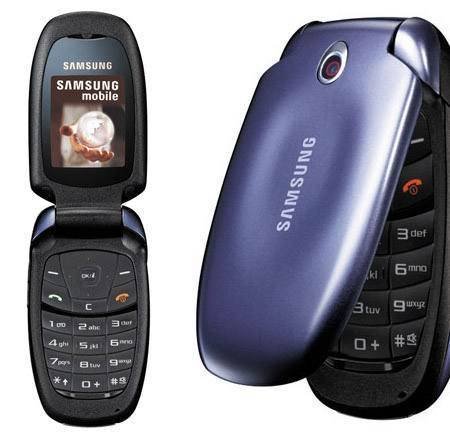
\includegraphics[trim={12mm 14mm 12mm 14mm},clip, width=\sizeP\textwidth]{fig/visual/ILSVRC2012_val_00000089.JPEG}&
	\fig[\sizeS]{visual/DeitBase_GradCAM_ILSVRC2012_val_00000089.png} &
	\fig[\sizeS]{visual/DeitBase_GradCAMPlusPlus_ILSVRC2012_val_00000089.png} &
	\fig[\sizeS]{visual/DeitBase_ScoreCAM_ILSVRC2012_val_00000089.png} &
	\fig[\sizeS]{visual/DeitBase_XGradCAM_ILSVRC2012_val_00000089.png} & 
        \fig[\sizeS]{visual/DeitBase_RawAttention_ILSVRC2012_val_00000089.png} &
        \fig[\sizeS]{visual/DeitBase_RolloutMean_ILSVRC2012_val_00000089.png} &
	\fig[\sizeS]{visual/DeitBase_OptiCAM_ILSVRC2012_val_00000089.png}  \\
	Cellphone &&&&&& \\
	\fig[\sizeS]{visual/ILSVRC2012_val_00000748.png}&
	\fig[\sizeS]{visual/DeitBase_GradCAM_ILSVRC2012_val_00000748.png} &
	\fig[\sizeS]{visual/DeitBase_GradCAMPlusPlus_ILSVRC2012_val_00000748.png} &
	\fig[\sizeS]{visual/DeitBase_ScoreCAM_ILSVRC2012_val_00000748.png} &
	\fig[\sizeS]{visual/DeitBase_XGradCAM_ILSVRC2012_val_00000748.png} & 
        \fig[\sizeS]{visual/DeitBase_RawAttention_ILSVRC2012_val_00000748.png} &
        \fig[\sizeS]{visual/DeitBase_RolloutMean_ILSVRC2012_val_00000748.png} &
	\fig[\sizeS]{visual/DeitBase_OptiCAM_ILSVRC2012_val_00000748.png}  \\
	Miniature Schnauzer &&&&&& \\
	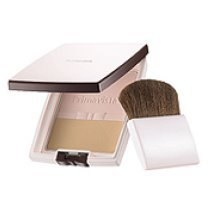
\includegraphics[trim={2mm 3mm 6mm 1mm},clip, width=\sizeP\textwidth]{fig/visual/ILSVRC2012_val_00000769.JPEG}&
	\fig[\sizeS]{visual/DeitBase_GradCAM_ILSVRC2012_val_00000769.png} &
	\fig[\sizeS]{visual/DeitBase_GradCAMPlusPlus_ILSVRC2012_val_00000769.png} &
	\fig[\sizeS]{visual/DeitBase_ScoreCAM_ILSVRC2012_val_00000769.png} &
	\fig[\sizeS]{visual/DeitBase_XGradCAM_ILSVRC2012_val_00000769.png} & 
        \fig[\sizeS]{visual/DeitBase_RawAttention_ILSVRC2012_val_00000769.png} &
        \fig[\sizeS]{visual/DeitBase_RolloutMean_ILSVRC2012_val_00000769.png} &
	\fig[\sizeS]{visual/DeitBase_OptiCAM_ILSVRC2012_val_00000769.png}  \\
	Face Powder &&&&&& \\
	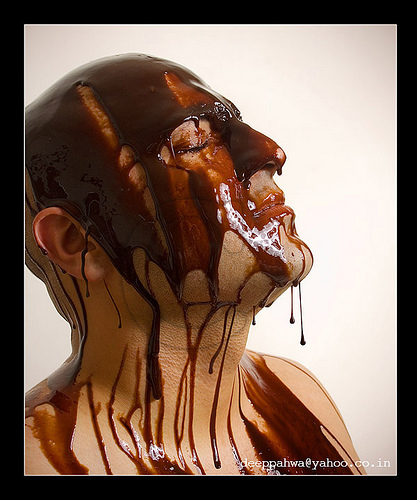
\includegraphics[trim={2mm 6mm 2mm 6mm},clip, width=\sizeP\textwidth]{fig/visual/ILSVRC2012_val_00000782.JPEG}&
	\fig[\sizeS]{visual/DeitBase_GradCAM_ILSVRC2012_val_00000782.png} &
	\fig[\sizeS]{visual/DeitBase_GradCAMPlusPlus_ILSVRC2012_val_00000782.png} &
	\fig[\sizeS]{visual/DeitBase_ScoreCAM_ILSVRC2012_val_00000782.png} &
	\fig[\sizeS]{visual/DeitBase_XGradCAM_ILSVRC2012_val_00000782.png} & 
        \fig[\sizeS]{visual/DeitBase_RawAttention_ILSVRC2012_val_00000782.png} &
        \fig[\sizeS]{visual/DeitBase_RolloutMean_ILSVRC2012_val_00000782.png} &
	\fig[\sizeS]{visual/DeitBase_OptiCAM_ILSVRC2012_val_00000782.png}  \\
	Chocolate Sauce &&&&&& \\
	\fig[\sizeS]{visual/ILSVRC2012_val_00001113.png}&
	\fig[\sizeS]{visual/DeitBase_GradCAM_ILSVRC2012_val_00001113.png} &
	\fig[\sizeS]{visual/DeitBase_GradCAMPlusPlus_ILSVRC2012_val_00001113.png} &
	\fig[\sizeS]{visual/DeitBase_ScoreCAM_ILSVRC2012_val_00001113.png} &
	\fig[\sizeS]{visual/DeitBase_XGradCAM_ILSVRC2012_val_00001113.png} & 
        \fig[\sizeS]{visual/DeitBase_RawAttention_ILSVRC2012_val_00001113.png} &
        \fig[\sizeS]{visual/DeitBase_RolloutMean_ILSVRC2012_val_00001113.png} &
	\fig[\sizeS]{visual/DeitBase_OptiCAM_ILSVRC2012_val_00001113.png}  \\
	Komondor &&&&&& \\
 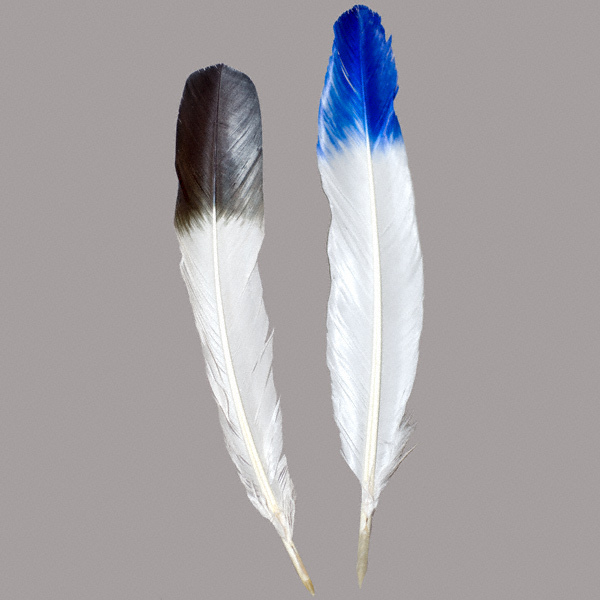
\includegraphics[trim={14mm 16mm 14mm 12mm},clip, width=\sizeP\textwidth]{fig/visual/ILSVRC2012_val_00001345.JPEG}&
	\fig[\sizeS]{visual/DeitBase_GradCAM_ILSVRC2012_val_00001345.png} &
	\fig[\sizeS]{visual/DeitBase_GradCAMPlusPlus_ILSVRC2012_val_00001345.png} &
	\fig[\sizeS]{visual/DeitBase_ScoreCAM_ILSVRC2012_val_00001345.png} &
	\fig[\sizeS]{visual/DeitBase_XGradCAM_ILSVRC2012_val_00001345.png} & 
        \fig[\sizeS]{visual/DeitBase_RawAttention_ILSVRC2012_val_00001345.png} &
        \fig[\sizeS]{visual/DeitBase_RolloutMean_ILSVRC2012_val_00001345.png} &
	\fig[\sizeS]{visual/DeitBase_OptiCAM_ILSVRC2012_val_00001345.png}  \\
	Quill &&&&&& \\
 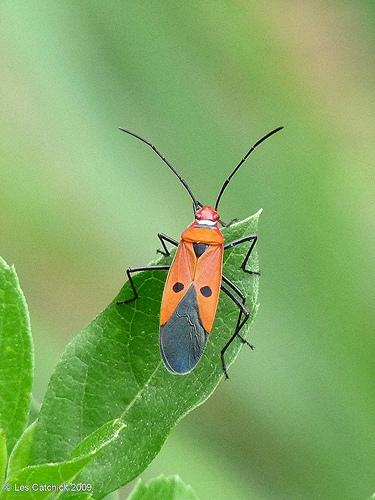
\includegraphics[trim={5mm 14mm 5mm 14mm},clip, width=\sizeP\textwidth]{fig/visual/ILSVRC2012_val_00001529.JPEG}&
	\fig[\sizeS]{visual/DeitBase_GradCAM_ILSVRC2012_val_00001529.png} &
	\fig[\sizeS]{visual/DeitBase_GradCAMPlusPlus_ILSVRC2012_val_00001529.png} &
	\fig[\sizeS]{visual/DeitBase_ScoreCAM_ILSVRC2012_val_00001529.png} &
	\fig[\sizeS]{visual/DeitBase_XGradCAM_ILSVRC2012_val_00001529.png} & 
        \fig[\sizeS]{visual/DeitBase_RawAttention_ILSVRC2012_val_00001529.png} &
        \fig[\sizeS]{visual/DeitBase_RolloutMean_ILSVRC2012_val_00001529.png} &
	\fig[\sizeS]{visual/DeitBase_OptiCAM_ILSVRC2012_val_00001529.png}  \\
	Longicorn &&&&&& \\
 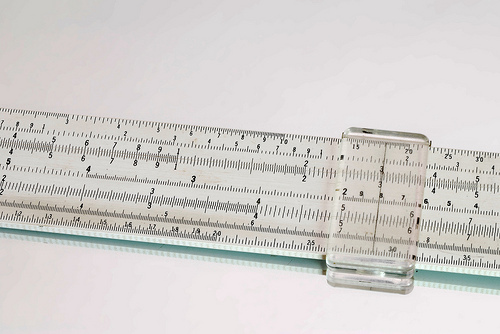
\includegraphics[trim={8mm 1mm 8mm 1mm},clip, width=\sizeP\textwidth]{fig/visual/ILSVRC2012_val_00001635.JPEG}&
	\fig[\sizeS]{visual/DeitBase_GradCAM_ILSVRC2012_val_00001635.png} &
	\fig[\sizeS]{visual/DeitBase_GradCAMPlusPlus_ILSVRC2012_val_00001635.png} &
	\fig[\sizeS]{visual/DeitBase_ScoreCAM_ILSVRC2012_val_00001635.png} &
	\fig[\sizeS]{visual/DeitBase_XGradCAM_ILSVRC2012_val_00001635.png} & 
        \fig[\sizeS]{visual/DeitBase_RawAttention_ILSVRC2012_val_00001635.png} &
        \fig[\sizeS]{visual/DeitBase_RolloutMean_ILSVRC2012_val_00001635.png} &
	\fig[\sizeS]{visual/DeitBase_OptiCAM_ILSVRC2012_val_00001635.png}  \\
	Slide Rule &&&&&& \\
\end{tabular}
\vspace{5pt}
\caption{Saliency maps obtained from ImageNet example images using different methods on DeiT.}
\label{fig:imagenet-vis-more-DeiT}
\end{figure*}

% % \begin{figure*}[t]
\newcommand{\sizeP}{.12}
\newcommand{\sizeS}{.12}
\newcommand{\hh}{.175\textwidth}
\newcommand{\ww}{.200\textwidth}
\tiny
\centering
\setlength{\tabcolsep}{1pt}
\begin{tabular}{cccccccc}
	Input image  &  Grad-CAM  & G-CAM++ & Score-CAM & XG-CAM & Raw Att. & Rollout & Opti-CAM (ours) \\
        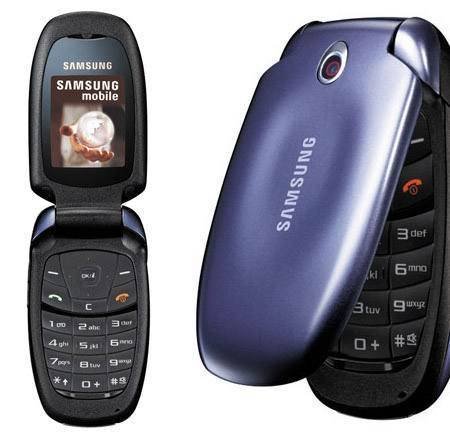
\includegraphics[trim={12mm 14mm 12mm 14mm},clip, width=\sizeP\textwidth]{fig/visual/ILSVRC2012_val_00000089.JPEG}&
	\fig[\sizeS]{visual/DeitTiny_GradCAM_ILSVRC2012_val_00000089.png} &
	\fig[\sizeS]{visual/DeitTiny_GradCAMPlusPlus_ILSVRC2012_val_00000089.png} &
	\fig[\sizeS]{visual/DeitTiny_ScoreCAM_ILSVRC2012_val_00000089.png} &
	\fig[\sizeS]{visual/DeitTiny_XGradCAM_ILSVRC2012_val_00000089.png} & 
        \fig[\sizeS]{visual/DeitTiny_RawAttention_ILSVRC2012_val_00000089.png} &
        \fig[\sizeS]{visual/DeitTiny_RolloutMean_ILSVRC2012_val_00000089.png} &
	\fig[\sizeS]{visual/DeitTiny_OptiCAM_ILSVRC2012_val_00000089.png}  \\
	Cellphone &&&&&& \\
	\fig[\sizeS]{visual/ILSVRC2012_val_00000748.png}&
	\fig[\sizeS]{visual/DeitTiny_GradCAM_ILSVRC2012_val_00000748.png} &
	\fig[\sizeS]{visual/DeitTiny_GradCAMPlusPlus_ILSVRC2012_val_00000748.png} &
	\fig[\sizeS]{visual/DeitTiny_ScoreCAM_ILSVRC2012_val_00000748.png} &
	\fig[\sizeS]{visual/DeitTiny_XGradCAM_ILSVRC2012_val_00000748.png} & 
        \fig[\sizeS]{visual/DeitTiny_RawAttention_ILSVRC2012_val_00000748.png} &
        \fig[\sizeS]{visual/DeitTiny_RolloutMean_ILSVRC2012_val_00000748.png} &
	\fig[\sizeS]{visual/DeitTiny_OptiCAM_ILSVRC2012_val_00000748.png}  \\
	Miniature Schnauzer &&&&&& \\
	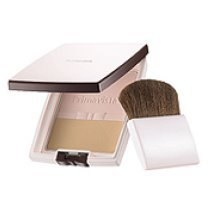
\includegraphics[trim={2mm 3mm 6mm 1mm},clip, width=\sizeP\textwidth]{fig/visual/ILSVRC2012_val_00000769.JPEG}&
	\fig[\sizeS]{visual/DeitTiny_GradCAM_ILSVRC2012_val_00000769.png} &
	\fig[\sizeS]{visual/DeitTiny_GradCAMPlusPlus_ILSVRC2012_val_00000769.png} &
	\fig[\sizeS]{visual/DeitTiny_ScoreCAM_ILSVRC2012_val_00000769.png} &
	\fig[\sizeS]{visual/DeitTiny_XGradCAM_ILSVRC2012_val_00000769.png} & 
        \fig[\sizeS]{visual/DeitTiny_RawAttention_ILSVRC2012_val_00000769.png} &
        \fig[\sizeS]{visual/DeitTiny_RolloutMean_ILSVRC2012_val_00000769.png} &
	\fig[\sizeS]{visual/DeitTiny_OptiCAM_ILSVRC2012_val_00000769.png}  \\
	Face Powder &&&&&& \\
	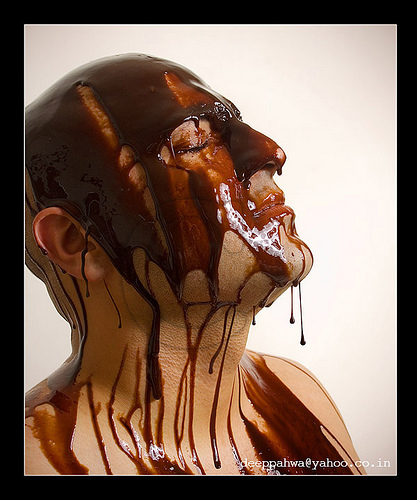
\includegraphics[trim={2mm 6mm 2mm 6mm},clip, width=\sizeP\textwidth]{fig/visual/ILSVRC2012_val_00000782.JPEG}&
	\fig[\sizeS]{visual/DeitTiny_GradCAM_ILSVRC2012_val_00000782.png} &
	\fig[\sizeS]{visual/DeitTiny_GradCAMPlusPlus_ILSVRC2012_val_00000782.png} &
	\fig[\sizeS]{visual/DeitTiny_ScoreCAM_ILSVRC2012_val_00000782.png} &
	\fig[\sizeS]{visual/DeitTiny_XGradCAM_ILSVRC2012_val_00000782.png} & 
        \fig[\sizeS]{visual/DeitTiny_RawAttention_ILSVRC2012_val_00000782.png} &
        \fig[\sizeS]{visual/DeitTiny_RolloutMean_ILSVRC2012_val_00000782.png} &
	\fig[\sizeS]{visual/DeitTiny_OptiCAM_ILSVRC2012_val_00000782.png}  \\
	Chocolate Sauce &&&&&& \\
	\fig[\sizeS]{visual/ILSVRC2012_val_00001113.png}&
	\fig[\sizeS]{visual/DeitTiny_GradCAM_ILSVRC2012_val_00001113.png} &
	\fig[\sizeS]{visual/DeitTiny_GradCAMPlusPlus_ILSVRC2012_val_00001113.png} &
	\fig[\sizeS]{visual/DeitTiny_ScoreCAM_ILSVRC2012_val_00001113.png} &
	\fig[\sizeS]{visual/DeitTiny_XGradCAM_ILSVRC2012_val_00001113.png} & 
        \fig[\sizeS]{visual/DeitTiny_RawAttention_ILSVRC2012_val_00001113.png} &
        \fig[\sizeS]{visual/DeitTiny_RolloutMean_ILSVRC2012_val_00001113.png} &
	\fig[\sizeS]{visual/DeitTiny_OptiCAM_ILSVRC2012_val_00001113.png}  \\
	Komondor &&&&&& \\
 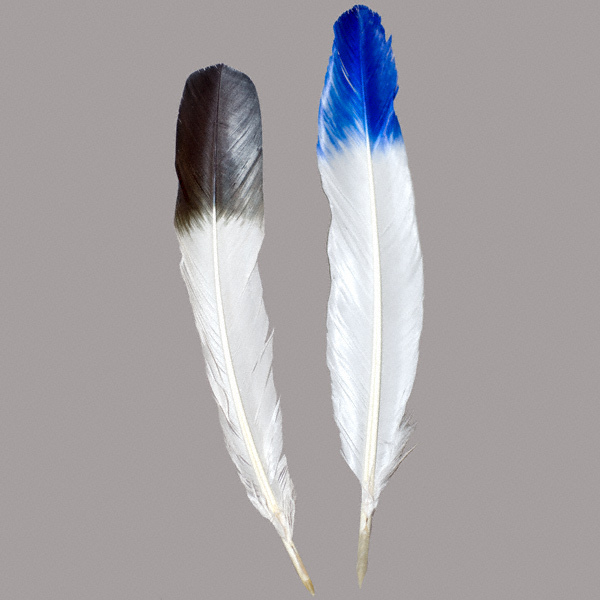
\includegraphics[trim={14mm 16mm 14mm 12mm},clip, width=\sizeP\textwidth]{fig/visual/ILSVRC2012_val_00001345.JPEG}&
	\fig[\sizeS]{visual/DeitTiny_GradCAM_ILSVRC2012_val_00001345.png} &
	\fig[\sizeS]{visual/DeitTiny_GradCAMPlusPlus_ILSVRC2012_val_00001345.png} &
	\fig[\sizeS]{visual/DeitTiny_ScoreCAM_ILSVRC2012_val_00001345.png} &
	\fig[\sizeS]{visual/DeitTiny_XGradCAM_ILSVRC2012_val_00001345.png} & 
        \fig[\sizeS]{visual/DeitTiny_RawAttention_ILSVRC2012_val_00001345.png} &
        \fig[\sizeS]{visual/DeitTiny_RolloutMean_ILSVRC2012_val_00001345.png} &
	\fig[\sizeS]{visual/DeitTiny_OptiCAM_ILSVRC2012_val_00001345.png}  \\
	Quill &&&&&& \\
 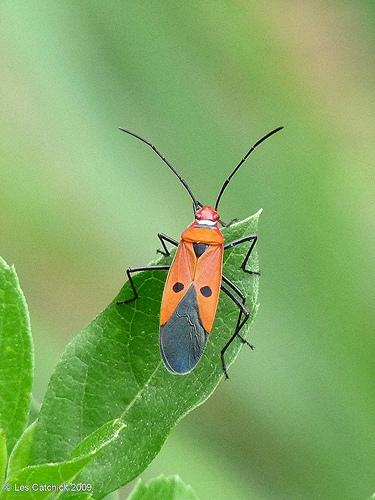
\includegraphics[trim={5mm 14mm 5mm 14mm},clip, width=\sizeP\textwidth]{fig/visual/ILSVRC2012_val_00001529.JPEG}&
	\fig[\sizeS]{visual/DeitTiny_GradCAM_ILSVRC2012_val_00001529.png} &
	\fig[\sizeS]{visual/DeitTiny_GradCAMPlusPlus_ILSVRC2012_val_00001529.png} &
	\fig[\sizeS]{visual/DeitTiny_ScoreCAM_ILSVRC2012_val_00001529.png} &
	\fig[\sizeS]{visual/DeitTiny_XGradCAM_ILSVRC2012_val_00001529.png} & 
        \fig[\sizeS]{visual/DeitTiny_RawAttention_ILSVRC2012_val_00001529.png} &
        \fig[\sizeS]{visual/DeitTiny_RolloutMean_ILSVRC2012_val_00001529.png} &
	\fig[\sizeS]{visual/DeitTiny_OptiCAM_ILSVRC2012_val_00001529.png}  \\
	Longicorn &&&&&& \\
 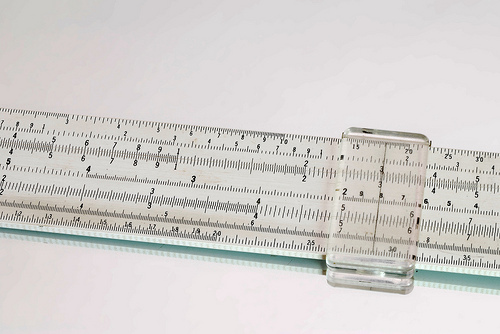
\includegraphics[trim={8mm 1mm 8mm 1mm},clip, width=\sizeP\textwidth]{fig/visual/ILSVRC2012_val_00001635.JPEG}&
	\fig[\sizeS]{visual/DeitTiny_GradCAM_ILSVRC2012_val_00001635.png} &
	\fig[\sizeS]{visual/DeitTiny_GradCAMPlusPlus_ILSVRC2012_val_00001635.png} &
	\fig[\sizeS]{visual/DeitTiny_ScoreCAM_ILSVRC2012_val_00001635.png} &
	\fig[\sizeS]{visual/DeitTiny_XGradCAM_ILSVRC2012_val_00001635.png} & 
        \fig[\sizeS]{visual/DeitTiny_RawAttention_ILSVRC2012_val_00001635.png} &
        \fig[\sizeS]{visual/DeitTiny_RolloutMean_ILSVRC2012_val_00001635.png} &
	\fig[\sizeS]{visual/DeitTiny_OptiCAM_ILSVRC2012_val_00001635.png}  \\
	Slide Rule &&&&&& \\
\end{tabular}
\vspace{5pt}
\caption{Saliency maps obtained from ImageNet example images using different methods on DeitTiny.}
\label{fig:imagenet-vis-more-DeitTiny}
\end{figure*}

% %------------------------------------------------------------------------------

% \section{More visualizations}
% \label{sec:more-vis}

% \autoref{fig:vis-chest-resnet} and \autoref{fig:vis-kvasir-resnet} present additional visualizations on Chest X-ray and Kvasir datasets using VGG16 and ResNet50. 
% Then \autoref{fig:imagenet-vis-more-vgg} and \autoref{fig:imagenet-vis-more-res}
% % \autoref{fig:imagenet-vis-more-vit} 
% show more results on ImageNet using VGG16 and ResNet50, respectively.

% Overall, we still observe that Opti-CAM captures more of the object area compared with other saliency methods and sometimes background context as well \autoref{fig:imagenet-vis-more-res}.



%\newpage

% ---- Bibliography ----
%
% BibTeX users should specify bibliography style 'splncs04'.
% References will then be sorted and formatted in the correct style.
%
% \clearpage
% \normalem
\bibliographystyle{elsarticle-num}
% \bibliography{cas-refs}
% \bibliographystyle{ieee}
\bibliography{refbib}

% 


\end{document}
